\documentclass{article}
\usepackage[left=1in,right=1in,bottom=1in,top=0.2in]{geometry}
\usepackage{newenviron, graphicx, amsmath, amssymb, enumerate}

\setcounter{MaxMatrixCols}{20}


\newcommand{\ferriswheel}{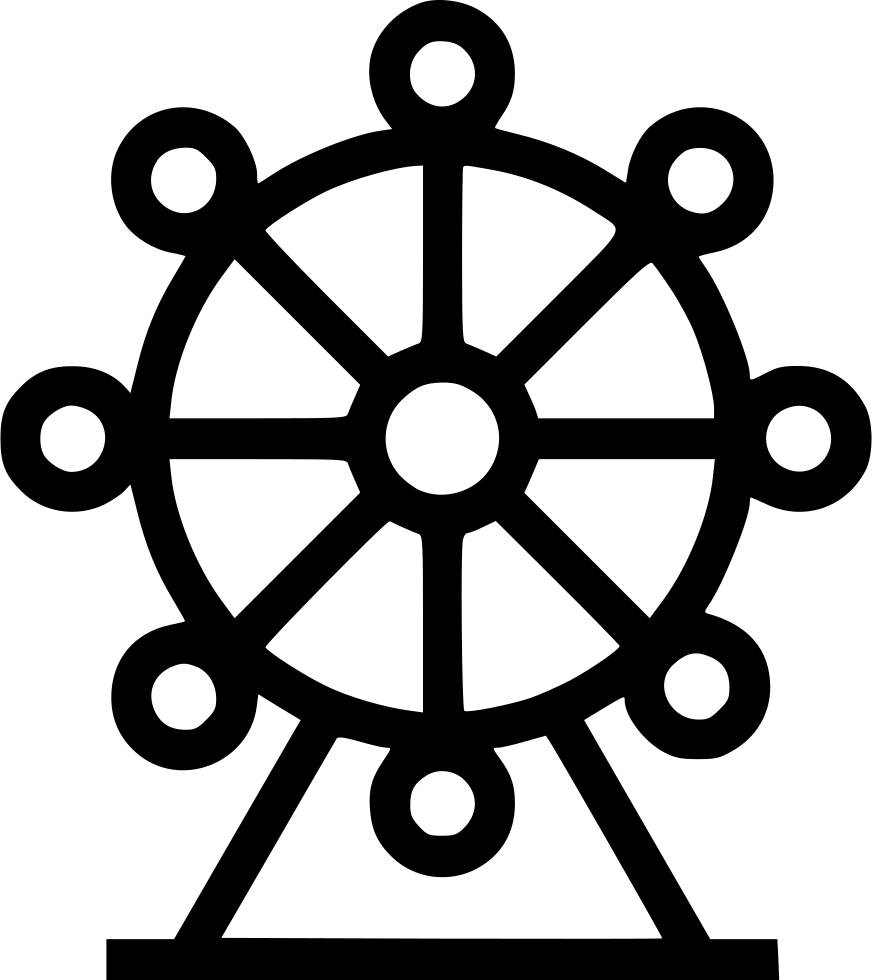
\includegraphics[scale=0.05]{ferris_wheel.png} }

\newenviron{exercise}[3]{
\ferriswheel \hfill  \begin{minipage}{0.7 \textwidth} \begin{center}
\Huge{\textbf{#1 \\ #2}}
\end{center}
\end{minipage} \hfill \ferriswheel
\ \\
\vspace{0.2in}

\exercisebody
\vfill \begin{flushright}Version {#3} \end{flushright} \newpage
}{}
\newenvironment{exerciseStatement}{}{}
\newenviron{exerciseAnswer}{}{}

\pagestyle{empty}

\begin{document}


\begin{exercise}{LE2}{Reduced row echelon form}{6107} 
\begin{exerciseStatement} 

\begin{enumerate}[(a)]
\item  

 For each of the following matrices, explain why it is not in reduced row echelon form. \[
                            A = \left[\begin{array}{cccc}
1 & 0 & -7 & 5 \\
0 & 1 & 0 & -3 \\
0 & 0 & 1 & -1 \\
0 & 0 & 0 & 0
\end{array}\right] \hspace{2em}
                            B = \left[\begin{array}{cccc}
1 & 0 & 2 & 0 \\
0 & -7 & -21 & 0 \\
0 & 0 & 0 & 1 \\
0 & 0 & 0 & 0
\end{array}\right] \hspace{2em}
                            C = \left[\begin{array}{cccc}
1 & 0 & 0 & -2 \\
0 & 0 & 1 & 1 \\
0 & 1 & 0 & 1 \\
0 & 0 & 0 & 0
\end{array}\right] \hspace{2em}
                        \hspace{2em}
                    \] 

 
\item  

 Show step-by-step why \[\operatorname{RREF}\left[\begin{array}{cccc}
5 & 2 & 5 & 16 \\
2 & 1 & 3 & 7 \\
-5 & -1 & 1 & -12 \\
1 & 0 & -5 & -2
\end{array}\right]=\left[\begin{array}{cccc}
1 & 0 & 0 & 3 \\
0 & 1 & 0 & -2 \\
0 & 0 & 1 & 1 \\
0 & 0 & 0 & 0
\end{array}\right]\]. 

 
\end{enumerate}

     \end{exerciseStatement}
 \begin{exerciseAnswer} 

\begin{itemize}
\item  

 \(A=\left[\begin{array}{cccc}
1 & 0 & -7 & 5 \\
0 & 1 & 0 & -3 \\
0 & 0 & 1 & -1 \\
0 & 0 & 0 & 0
\end{array}\right]\) is not in reduced row echelon form because not every entry above and below each pivot is zero. 

 
\item  

 \(B=\left[\begin{array}{cccc}
1 & 0 & 2 & 0 \\
0 & -7 & -21 & 0 \\
0 & 0 & 0 & 1 \\
0 & 0 & 0 & 0
\end{array}\right]\) is not in reduced row echelon form because the pivots are not all \(1\). 

 
\item  

 \(C=\left[\begin{array}{cccc}
1 & 0 & 0 & -2 \\
0 & 0 & 1 & 1 \\
0 & 1 & 0 & 1 \\
0 & 0 & 0 & 0
\end{array}\right]\) is not in reduced row echelon form because the pivots are not descending to the right. 

 
\end{itemize}

     \end{exerciseAnswer}
 \end{exercise}


\begin{exercise}{LE2}{Reduced row echelon form}{2847} 
\begin{exerciseStatement} 

\begin{enumerate}[(a)]
\item  

 For each of the following matrices, explain why it is not in reduced row echelon form. \[
                            A = \left[\begin{array}{ccccc}
1 & 4 & 3 & 3 & -5 \\
0 & 0 & 0 & 1 & -2 \\
0 & 0 & 0 & 0 & 0
\end{array}\right] \hspace{2em}
                            B = \left[\begin{array}{ccccc}
0 & 1 & 1 & 2 & -1 \\
1 & 0 & 2 & -2 & -1 \\
0 & 0 & 0 & 0 & 0
\end{array}\right] \hspace{2em}
                            C = \left[\begin{array}{ccccc}
3 & 12 & 0 & -6 & 0 \\
0 & 0 & 1 & 1 & -2 \\
0 & 0 & 0 & 0 & 0
\end{array}\right] \hspace{2em}
                        \hspace{2em}
                    \] 

 
\item  

 Show step-by-step why \[\operatorname{RREF}\left[\begin{array}{ccccc}
1 & 2 & -3 & -2 & 5 \\
-1 & -2 & 3 & 2 & -4 \\
1 & 2 & -3 & -2 & 4
\end{array}\right]=\left[\begin{array}{ccccc}
1 & 2 & -3 & -2 & 0 \\
0 & 0 & 0 & 0 & 1 \\
0 & 0 & 0 & 0 & 0
\end{array}\right]\]. 

 
\end{enumerate}

     \end{exerciseStatement}
 \begin{exerciseAnswer} 

\begin{itemize}
\item  

 \(A=\left[\begin{array}{ccccc}
1 & 4 & 3 & 3 & -5 \\
0 & 0 & 0 & 1 & -2 \\
0 & 0 & 0 & 0 & 0
\end{array}\right]\) is not in reduced row echelon form because not every entry above and below each pivot is zero. 

 
\item  

 \(B=\left[\begin{array}{ccccc}
0 & 1 & 1 & 2 & -1 \\
1 & 0 & 2 & -2 & -1 \\
0 & 0 & 0 & 0 & 0
\end{array}\right]\) is not in reduced row echelon form because the pivots are not descending to the right. 

 
\item  

 \(C=\left[\begin{array}{ccccc}
3 & 12 & 0 & -6 & 0 \\
0 & 0 & 1 & 1 & -2 \\
0 & 0 & 0 & 0 & 0
\end{array}\right]\) is not in reduced row echelon form because the pivots are not all \(1\). 

 
\end{itemize}

     \end{exerciseAnswer}
 \end{exercise}


\begin{exercise}{LE2}{Reduced row echelon form}{3245} 
\begin{exerciseStatement} 

\begin{enumerate}[(a)]
\item  

 For each of the following matrices, explain why it is not in reduced row echelon form. \[
                            A = \left[\begin{array}{cccc}
1 & 0 & -3 & 3 \\
5 & 1 & -15 & 12 \\
0 & 0 & 0 & 0 \\
0 & 0 & 0 & 0
\end{array}\right] \hspace{2em}
                            B = \left[\begin{array}{cccc}
0 & 1 & 2 & 2 \\
1 & 0 & -2 & -3 \\
0 & 0 & 0 & 0 \\
0 & 0 & 0 & 0
\end{array}\right] \hspace{2em}
                            C = \left[\begin{array}{cccc}
1 & -5 & 0 & 1 \\
0 & 0 & 5 & 10 \\
0 & 0 & 0 & 0 \\
0 & 0 & 0 & 0
\end{array}\right] \hspace{2em}
                        \hspace{2em}
                    \] 

 
\item  

 Show step-by-step why \[\operatorname{RREF}\left[\begin{array}{cccc}
-3 & 3 & -6 & -2 \\
2 & -2 & 4 & 1 \\
-3 & 3 & -6 & -2 \\
-4 & 4 & -8 & -3
\end{array}\right]=\left[\begin{array}{cccc}
1 & -1 & 2 & 0 \\
0 & 0 & 0 & 1 \\
0 & 0 & 0 & 0 \\
0 & 0 & 0 & 0
\end{array}\right]\]. 

 
\end{enumerate}

     \end{exerciseStatement}
 \begin{exerciseAnswer} 

\begin{itemize}
\item  

 \(A=\left[\begin{array}{cccc}
1 & 0 & -3 & 3 \\
5 & 1 & -15 & 12 \\
0 & 0 & 0 & 0 \\
0 & 0 & 0 & 0
\end{array}\right]\) is not in reduced row echelon form because not every entry above and below each pivot is zero. 

 
\item  

 \(B=\left[\begin{array}{cccc}
0 & 1 & 2 & 2 \\
1 & 0 & -2 & -3 \\
0 & 0 & 0 & 0 \\
0 & 0 & 0 & 0
\end{array}\right]\) is not in reduced row echelon form because the pivots are not descending to the right. 

 
\item  

 \(C=\left[\begin{array}{cccc}
1 & -5 & 0 & 1 \\
0 & 0 & 5 & 10 \\
0 & 0 & 0 & 0 \\
0 & 0 & 0 & 0
\end{array}\right]\) is not in reduced row echelon form because the pivots are not all \(1\). 

 
\end{itemize}

     \end{exerciseAnswer}
 \end{exercise}


\begin{exercise}{LE2}{Reduced row echelon form}{6207} 
\begin{exerciseStatement} 

\begin{enumerate}[(a)]
\item  

 For each of the following matrices, explain why it is not in reduced row echelon form. \[
                            A = \left[\begin{array}{cccc}
1 & 0 & 0 & -1 \\
0 & 1 & 0 & 2 \\
0 & 0 & 3 & 6 \\
0 & 0 & 0 & 0
\end{array}\right] \hspace{2em}
                            B = \left[\begin{array}{cccc}
1 & 0 & 0 & 2 \\
0 & 1 & 0 & -1 \\
3 & 0 & 1 & 7 \\
0 & 0 & 0 & 0
\end{array}\right] \hspace{2em}
                            C = \left[\begin{array}{cccc}
1 & 0 & 0 & -2 \\
0 & 0 & 1 & -2 \\
0 & 1 & 0 & 1 \\
0 & 0 & 0 & 0
\end{array}\right] \hspace{2em}
                        \hspace{2em}
                    \] 

 
\item  

 Show step-by-step why \[\operatorname{RREF}\left[\begin{array}{cccc}
-2 & -4 & 4 & 5 \\
1 & 2 & -1 & -2 \\
1 & 2 & -2 & -3 \\
0 & 0 & 3 & 5
\end{array}\right]=\left[\begin{array}{cccc}
1 & 2 & 0 & 0 \\
0 & 0 & 1 & 0 \\
0 & 0 & 0 & 1 \\
0 & 0 & 0 & 0
\end{array}\right]\]. 

 
\end{enumerate}

     \end{exerciseStatement}
 \begin{exerciseAnswer} 

\begin{itemize}
\item  

 \(A=\left[\begin{array}{cccc}
1 & 0 & 0 & -1 \\
0 & 1 & 0 & 2 \\
0 & 0 & 3 & 6 \\
0 & 0 & 0 & 0
\end{array}\right]\) is not in reduced row echelon form because the pivots are not all \(1\). 

 
\item  

 \(B=\left[\begin{array}{cccc}
1 & 0 & 0 & 2 \\
0 & 1 & 0 & -1 \\
3 & 0 & 1 & 7 \\
0 & 0 & 0 & 0
\end{array}\right]\) is not in reduced row echelon form because not every entry above and below each pivot is zero. 

 
\item  

 \(C=\left[\begin{array}{cccc}
1 & 0 & 0 & -2 \\
0 & 0 & 1 & -2 \\
0 & 1 & 0 & 1 \\
0 & 0 & 0 & 0
\end{array}\right]\) is not in reduced row echelon form because the pivots are not descending to the right. 

 
\end{itemize}

     \end{exerciseAnswer}
 \end{exercise}


\begin{exercise}{LE2}{Reduced row echelon form}{6447} 
\begin{exerciseStatement} 

\begin{enumerate}[(a)]
\item  

 For each of the following matrices, explain why it is not in reduced row echelon form. \[
                            A = \left[\begin{array}{ccc}
1 & 6 & -14 \\
0 & 1 & -2 \\
0 & 0 & 0 \\
0 & 0 & 0 \\
0 & 0 & 0
\end{array}\right] \hspace{2em}
                            B = \left[\begin{array}{ccc}
0 & 1 & -3 \\
1 & 0 & 1 \\
0 & 0 & 0 \\
0 & 0 & 0 \\
0 & 0 & 0
\end{array}\right] \hspace{2em}
                            C = \left[\begin{array}{ccc}
1 & 0 & -1 \\
0 & 6 & 0 \\
0 & 0 & 0 \\
0 & 0 & 0 \\
0 & 0 & 0
\end{array}\right] \hspace{2em}
                        \hspace{2em}
                    \] 

 
\item  

 Show step-by-step why \[\operatorname{RREF}\left[\begin{array}{ccc}
-1 & -2 & 4 \\
1 & 4 & -10 \\
2 & 5 & -11 \\
1 & 1 & -1 \\
0 & -3 & 9
\end{array}\right]=\left[\begin{array}{ccc}
1 & 0 & 2 \\
0 & 1 & -3 \\
0 & 0 & 0 \\
0 & 0 & 0 \\
0 & 0 & 0
\end{array}\right]\]. 

 
\end{enumerate}

     \end{exerciseStatement}
 \begin{exerciseAnswer} 

\begin{itemize}
\item  

 \(A=\left[\begin{array}{ccc}
1 & 6 & -14 \\
0 & 1 & -2 \\
0 & 0 & 0 \\
0 & 0 & 0 \\
0 & 0 & 0
\end{array}\right]\) is not in reduced row echelon form because not every entry above and below each pivot is zero. 

 
\item  

 \(B=\left[\begin{array}{ccc}
0 & 1 & -3 \\
1 & 0 & 1 \\
0 & 0 & 0 \\
0 & 0 & 0 \\
0 & 0 & 0
\end{array}\right]\) is not in reduced row echelon form because the pivots are not descending to the right. 

 
\item  

 \(C=\left[\begin{array}{ccc}
1 & 0 & -1 \\
0 & 6 & 0 \\
0 & 0 & 0 \\
0 & 0 & 0 \\
0 & 0 & 0
\end{array}\right]\) is not in reduced row echelon form because the pivots are not all \(1\). 

 
\end{itemize}

     \end{exerciseAnswer}
 \end{exercise}


\begin{exercise}{LE3}{Counting Solutions for Linear Systems}{7098} 
\begin{exerciseStatement} 

 Consider each of the following systems of linear equations or vector equations. 

 

\begin{enumerate}[(a)]
\item  

 \[
              x_{1} \left[\begin{array}{c}
1 \\
2 \\
4
\end{array}\right] + x_{2} \left[\begin{array}{c}
2 \\
5 \\
4
\end{array}\right] + x_{3} \left[\begin{array}{c}
4 \\
9 \\
12
\end{array}\right] = \left[\begin{array}{c}
-8 \\
-20 \\
-23
\end{array}\right]
            \] 

 
\item  

 \[
              x_{1} \left[\begin{array}{c}
-2 \\
-3 \\
-5
\end{array}\right] + x_{2} \left[\begin{array}{c}
4 \\
6 \\
10
\end{array}\right] + x_{3} \left[\begin{array}{c}
-1 \\
-2 \\
-5
\end{array}\right] = \left[\begin{array}{c}
-1 \\
-3 \\
-10
\end{array}\right]
            \] 

 
\item  

 \[
              \begin{matrix}
 -2 \, x_{1} &  -  & x_{2} &  +  & x_{3} & = & 9 \\
 3 \, x_{1} &  +  & x_{2} &  -  & 4 \, x_{3} & = & -15 \\
 -3 \, x_{1} &  -  & x_{2} &  +  & 5 \, x_{3} & = & 16 \\
 \end{matrix}
            \] 

 
\end{enumerate}

     

\begin{itemize}
\item  

 Explain how to find a simpler system or vector equation that has the same solution set for each. 

 
\item  

 Explain whether each solution set has no solutions, one solution, or infinitely-many solutions. If the set is finite, describe it using set notation. 

 
\end{itemize}

     \end{exerciseStatement}
 \begin{exerciseAnswer} 

\begin{enumerate}[(a)]
\item  

 \[\mathrm{RREF}\left[\begin{array}{ccc|c}
1 & 2 & 4 & -8 \\
2 & 5 & 9 & -20 \\
4 & 4 & 12 & -23
\end{array}\right]=\left[\begin{array}{ccc|c}
1 & 0 & 2 & 0 \\
0 & 1 & 1 & 0 \\
0 & 0 & 0 & 1
\end{array}\right]\] The solution set has no solutions. The solution set is \(\emptyset\). 

 
\item  

 \[\mathrm{RREF}\left[\begin{array}{ccc|c}
-2 & 4 & -1 & -1 \\
-3 & 6 & -2 & -3 \\
-5 & 10 & -5 & -10
\end{array}\right]=\left[\begin{array}{ccc|c}
1 & -2 & 0 & -1 \\
0 & 0 & 1 & 3 \\
0 & 0 & 0 & 0
\end{array}\right]\] The solution set has infinitely-many solutions. 

 
\item  

 \[\mathrm{RREF}\left[\begin{array}{ccc|c}
-2 & -1 & 1 & 9 \\
3 & 1 & -4 & -15 \\
-3 & -1 & 5 & 16
\end{array}\right]=\left[\begin{array}{ccc|c}
1 & 0 & 0 & -3 \\
0 & 1 & 0 & -2 \\
0 & 0 & 1 & 1
\end{array}\right]\] The solution set has one solution. The solution set is \(\left\{ \left[\begin{array}{c}
-3 \\
-2 \\
1
\end{array}\right] \right\}\). 

 
\end{enumerate}

     \end{exerciseAnswer}
 \end{exercise}


\begin{exercise}{LE3}{Counting Solutions for Linear Systems}{7332} 
\begin{exerciseStatement} 

 Consider each of the following systems of linear equations or vector equations. 

 

\begin{enumerate}[(a)]
\item  

 \[
              x_{1} \left[\begin{array}{c}
-1 \\
-2 \\
0
\end{array}\right] + x_{2} \left[\begin{array}{c}
2 \\
3 \\
1
\end{array}\right] + x_{3} \left[\begin{array}{c}
-2 \\
-5 \\
2
\end{array}\right] = \left[\begin{array}{c}
-7 \\
-14 \\
1
\end{array}\right]
            \] 

 
\item  

 \[
              \begin{matrix}
 5 \, x_{1} &  &  &  -  & 10 \, x_{3} & = & 16 \\
 3 \, x_{1} &  +  & x_{2} &  -  & 6 \, x_{3} & = & 8 \\
 -2 \, x_{1} &  &  &  +  & 4 \, x_{3} & = & -7 \\
 \end{matrix}
            \] 

 
\item  

 \[
              \begin{matrix}
 -x_{1} &  +  & 2 \, x_{2} &  +  & 4 \, x_{3} & = & 3 \\
 2 \, x_{1} &  -  & 5 \, x_{2} &  -  & 11 \, x_{3} & = & -7 \\
 -3 \, x_{1} &  +  & 5 \, x_{2} &  +  & 9 \, x_{3} & = & 8 \\
 \end{matrix}
            \] 

 
\end{enumerate}

     

\begin{itemize}
\item  

 Explain how to find a simpler system or vector equation that has the same solution set for each. 

 
\item  

 Explain whether each solution set has no solutions, one solution, or infinitely-many solutions. If the set is finite, describe it using set notation. 

 
\end{itemize}

     \end{exerciseStatement}
 \begin{exerciseAnswer} 

\begin{enumerate}[(a)]
\item  

 \[\mathrm{RREF}\left[\begin{array}{ccc|c}
-1 & 2 & -2 & -7 \\
-2 & 3 & -5 & -14 \\
0 & 1 & 2 & 1
\end{array}\right]=\left[\begin{array}{ccc|c}
1 & 0 & 0 & 3 \\
0 & 1 & 0 & -1 \\
0 & 0 & 1 & 1
\end{array}\right]\] The solution set has one solution. The solution set is \(\left\{ \left[\begin{array}{c}
3 \\
-1 \\
1
\end{array}\right] \right\}\). 

 
\item  

 \[\mathrm{RREF}\left[\begin{array}{ccc|c}
5 & 0 & -10 & 16 \\
3 & 1 & -6 & 8 \\
-2 & 0 & 4 & -7
\end{array}\right]=\left[\begin{array}{ccc|c}
1 & 0 & -2 & 0 \\
0 & 1 & 0 & 0 \\
0 & 0 & 0 & 1
\end{array}\right]\] The solution set has no solutions. The solution set is \(\emptyset\). 

 
\item  

 \[\mathrm{RREF}\left[\begin{array}{ccc|c}
-1 & 2 & 4 & 3 \\
2 & -5 & -11 & -7 \\
-3 & 5 & 9 & 8
\end{array}\right]=\left[\begin{array}{ccc|c}
1 & 0 & 2 & -1 \\
0 & 1 & 3 & 1 \\
0 & 0 & 0 & 0
\end{array}\right]\] The solution set has infinitely-many solutions. 

 
\end{enumerate}

     \end{exerciseAnswer}
 \end{exercise}


\begin{exercise}{LE3}{Counting Solutions for Linear Systems}{9916} 
\begin{exerciseStatement} 

 Consider each of the following systems of linear equations or vector equations. 

 

\begin{enumerate}[(a)]
\item  

 \[
              x_{1} \left[\begin{array}{c}
-3 \\
4 \\
0
\end{array}\right] + x_{2} \left[\begin{array}{c}
-4 \\
5 \\
1
\end{array}\right] + x_{3} \left[\begin{array}{c}
-3 \\
3 \\
4
\end{array}\right] = \left[\begin{array}{c}
-3 \\
4 \\
-1
\end{array}\right]
            \] 

 
\item  

 \[
              x_{1} \left[\begin{array}{c}
4 \\
1 \\
0
\end{array}\right] + x_{2} \left[\begin{array}{c}
8 \\
2 \\
0
\end{array}\right] + x_{3} \left[\begin{array}{c}
-5 \\
-1 \\
4
\end{array}\right] = \left[\begin{array}{c}
-13 \\
-3 \\
4
\end{array}\right]
            \] 

 
\item  

 \[
              \begin{matrix}
 x_{1} &  &  &  -  & 2 \, x_{3} & = & -2 \\
 -3 \, x_{1} &  +  & x_{2} &  +  & 3 \, x_{3} & = & 9 \\
 -2 \, x_{1} &  +  & 5 \, x_{2} &  -  & 11 \, x_{3} & = & 12 \\
 \end{matrix}
            \] 

 
\end{enumerate}

     

\begin{itemize}
\item  

 Explain how to find a simpler system or vector equation that has the same solution set for each. 

 
\item  

 Explain whether each solution set has no solutions, one solution, or infinitely-many solutions. If the set is finite, describe it using set notation. 

 
\end{itemize}

     \end{exerciseStatement}
 \begin{exerciseAnswer} 

\begin{enumerate}[(a)]
\item  

 \[\mathrm{RREF}\left[\begin{array}{ccc|c}
-3 & -4 & -3 & -3 \\
4 & 5 & 3 & 4 \\
0 & 1 & 4 & -1
\end{array}\right]=\left[\begin{array}{ccc|c}
1 & 0 & 0 & -2 \\
0 & 1 & 0 & 3 \\
0 & 0 & 1 & -1
\end{array}\right]\] The solution set has one solution. The solution set is \(\left\{ \left[\begin{array}{c}
-2 \\
3 \\
-1
\end{array}\right] \right\}\). 

 
\item  

 \[\mathrm{RREF}\left[\begin{array}{ccc|c}
4 & 8 & -5 & -13 \\
1 & 2 & -1 & -3 \\
0 & 0 & 4 & 4
\end{array}\right]=\left[\begin{array}{ccc|c}
1 & 2 & 0 & -2 \\
0 & 0 & 1 & 1 \\
0 & 0 & 0 & 0
\end{array}\right]\] The solution set has infinitely-many solutions. 

 
\item  

 \[\mathrm{RREF}\left[\begin{array}{ccc|c}
1 & 0 & -2 & -2 \\
-3 & 1 & 3 & 9 \\
-2 & 5 & -11 & 12
\end{array}\right]=\left[\begin{array}{ccc|c}
1 & 0 & -2 & 0 \\
0 & 1 & -3 & 0 \\
0 & 0 & 0 & 1
\end{array}\right]\] The solution set has no solutions. The solution set is \(\emptyset\). 

 
\end{enumerate}

     \end{exerciseAnswer}
 \end{exercise}


\begin{exercise}{LE3}{Counting Solutions for Linear Systems}{6779} 
\begin{exerciseStatement} 

 Consider each of the following systems of linear equations or vector equations. 

 

\begin{enumerate}[(a)]
\item  

 \[
              x_{1} \left[\begin{array}{c}
1 \\
-3 \\
0
\end{array}\right] + x_{2} \left[\begin{array}{c}
-3 \\
-5 \\
-5
\end{array}\right] + x_{3} \left[\begin{array}{c}
9 \\
15 \\
15
\end{array}\right] = \left[\begin{array}{c}
11 \\
5 \\
16
\end{array}\right]
            \] 

 
\item  

 \[
              \begin{matrix}
 -3 \, x_{1} &  +  & 4 \, x_{2} &  -  & 4 \, x_{3} & = & -13 \\
 &  & x_{2} &  -  & 3 \, x_{3} & = & -6 \\
 -2 \, x_{1} &  +  & 3 \, x_{2} &  -  & 4 \, x_{3} & = & -11 \\
 \end{matrix}
            \] 

 
\item  

 \[
              x_{1} \left[\begin{array}{c}
5 \\
-2 \\
-4
\end{array}\right] + x_{2} \left[\begin{array}{c}
-5 \\
2 \\
4
\end{array}\right] + x_{3} \left[\begin{array}{c}
3 \\
-1 \\
1
\end{array}\right] = \left[\begin{array}{c}
4 \\
-1 \\
7
\end{array}\right]
            \] 

 
\end{enumerate}

     

\begin{itemize}
\item  

 Explain how to find a simpler system or vector equation that has the same solution set for each. 

 
\item  

 Explain whether each solution set has no solutions, one solution, or infinitely-many solutions. If the set is finite, describe it using set notation. 

 
\end{itemize}

     \end{exerciseStatement}
 \begin{exerciseAnswer} 

\begin{enumerate}[(a)]
\item  

 \[\mathrm{RREF}\left[\begin{array}{ccc|c}
1 & -3 & 9 & 11 \\
-3 & -5 & 15 & 5 \\
0 & -5 & 15 & 16
\end{array}\right]=\left[\begin{array}{ccc|c}
1 & 0 & 0 & 0 \\
0 & 1 & -3 & 0 \\
0 & 0 & 0 & 1
\end{array}\right]\] The solution set has no solutions. The solution set is \(\emptyset\). 

 
\item  

 \[\mathrm{RREF}\left[\begin{array}{ccc|c}
-3 & 4 & -4 & -13 \\
0 & 1 & -3 & -6 \\
-2 & 3 & -4 & -11
\end{array}\right]=\left[\begin{array}{ccc|c}
1 & 0 & 0 & -1 \\
0 & 1 & 0 & -3 \\
0 & 0 & 1 & 1
\end{array}\right]\] The solution set has one solution. The solution set is \(\left\{ \left[\begin{array}{c}
-1 \\
-3 \\
1
\end{array}\right] \right\}\). 

 
\item  

 \[\mathrm{RREF}\left[\begin{array}{ccc|c}
5 & -5 & 3 & 4 \\
-2 & 2 & -1 & -1 \\
-4 & 4 & 1 & 7
\end{array}\right]=\left[\begin{array}{ccc|c}
1 & -1 & 0 & -1 \\
0 & 0 & 1 & 3 \\
0 & 0 & 0 & 0
\end{array}\right]\] The solution set has infinitely-many solutions. 

 
\end{enumerate}

     \end{exerciseAnswer}
 \end{exercise}


\begin{exercise}{LE3}{Counting Solutions for Linear Systems}{7000} 
\begin{exerciseStatement} 

 Consider each of the following systems of linear equations or vector equations. 

 

\begin{enumerate}[(a)]
\item  

 \[
              \begin{matrix}
 -2 \, x_{1} &  +  & 5 \, x_{2} &  -  & 8 \, x_{3} & = & 7 \\
 -x_{1} &  +  & 2 \, x_{2} &  -  & 3 \, x_{3} & = & 1 \\
 -2 \, x_{1} &  +  & 2 \, x_{2} &  -  & 2 \, x_{3} & = & 1 \\
 \end{matrix}
            \] 

 
\item  

 \[
              x_{1} \left[\begin{array}{c}
1 \\
0 \\
0
\end{array}\right] + x_{2} \left[\begin{array}{c}
3 \\
1 \\
3
\end{array}\right] + x_{3} \left[\begin{array}{c}
-3 \\
-1 \\
-2
\end{array}\right] = \left[\begin{array}{c}
5 \\
1 \\
5
\end{array}\right]
            \] 

 
\item  

 \[
              \begin{matrix}
 &  -  & x_{2} &  -  & 2 \, x_{3} & = & -3 \\
 x_{1} &  +  & 3 \, x_{2} &  +  & 6 \, x_{3} & = & 11 \\
 x_{1} &  -  & 2 \, x_{2} &  -  & 4 \, x_{3} & = & -4 \\
 \end{matrix}
            \] 

 
\end{enumerate}

     

\begin{itemize}
\item  

 Explain how to find a simpler system or vector equation that has the same solution set for each. 

 
\item  

 Explain whether each solution set has no solutions, one solution, or infinitely-many solutions. If the set is finite, describe it using set notation. 

 
\end{itemize}

     \end{exerciseStatement}
 \begin{exerciseAnswer} 

\begin{enumerate}[(a)]
\item  

 \[\mathrm{RREF}\left[\begin{array}{ccc|c}
-2 & 5 & -8 & 7 \\
-1 & 2 & -3 & 1 \\
-2 & 2 & -2 & 1
\end{array}\right]=\left[\begin{array}{ccc|c}
1 & 0 & -1 & 0 \\
0 & 1 & -2 & 0 \\
0 & 0 & 0 & 1
\end{array}\right]\] The solution set has no solutions. The solution set is \(\emptyset\). 

 
\item  

 \[\mathrm{RREF}\left[\begin{array}{ccc|c}
1 & 3 & -3 & 5 \\
0 & 1 & -1 & 1 \\
0 & 3 & -2 & 5
\end{array}\right]=\left[\begin{array}{ccc|c}
1 & 0 & 0 & 2 \\
0 & 1 & 0 & 3 \\
0 & 0 & 1 & 2
\end{array}\right]\] The solution set has one solution. The solution set is \(\left\{ \left[\begin{array}{c}
2 \\
3 \\
2
\end{array}\right] \right\}\). 

 
\item  

 \[\mathrm{RREF}\left[\begin{array}{ccc|c}
0 & -1 & -2 & -3 \\
1 & 3 & 6 & 11 \\
1 & -2 & -4 & -4
\end{array}\right]=\left[\begin{array}{ccc|c}
1 & 0 & 0 & 2 \\
0 & 1 & 2 & 3 \\
0 & 0 & 0 & 0
\end{array}\right]\] The solution set has infinitely-many solutions. 

 
\end{enumerate}

     \end{exerciseAnswer}
 \end{exercise}


\begin{exercise}{LE4}{Linear Systems with Infinitely-Many Solutions}{4455} 
\begin{exerciseStatement} 

 Consider the following vector equation. \[       
        x_{1} \left[\begin{array}{c}
1 \\
-2 \\
0 \\
2
\end{array}\right] + x_{2} \left[\begin{array}{c}
3 \\
-5 \\
-3 \\
4
\end{array}\right] + x_{3} \left[\begin{array}{c}
4 \\
-7 \\
-3 \\
6
\end{array}\right] = \left[\begin{array}{c}
1 \\
-1 \\
-3 \\
0
\end{array}\right]
      \] 

 

\begin{enumerate}[(a)]
\item  

 Explain how to find a simpler system or vector equation that has the same solution set. 

 
\item  

 Explain how to describe this solution set using set notation. 

 
\end{enumerate}

     \end{exerciseStatement}
 \begin{exerciseAnswer} 

 \[\mathrm{RREF}\left[\begin{array}{ccc|c}
1 & 3 & 4 & 1 \\
-2 & -5 & -7 & -1 \\
0 & -3 & -3 & -3 \\
2 & 4 & 6 & 0
\end{array}\right]=\left[\begin{array}{ccc|c}
1 & 0 & 1 & -2 \\
0 & 1 & 1 & 1 \\
0 & 0 & 0 & 0 \\
0 & 0 & 0 & 0
\end{array}\right]\] The solution set is \( \left\{ \left[\begin{array}{c}
-a - 2 \\
-a + 1 \\
a
\end{array}\right] \,\middle|\, a \in\mathbb R \right\} \). 

 \end{exerciseAnswer}
 \end{exercise}


\begin{exercise}{LE4}{Linear Systems with Infinitely-Many Solutions}{7397} 
\begin{exerciseStatement} 

 Consider the following system of linear equations. \[
        \begin{matrix}
 5 \, x_{1} &  +  & 10 \, x_{2} &  -  & 3 \, x_{3} &  -  & 7 \, x_{4} & = & -8 \\
 3 \, x_{1} &  +  & 6 \, x_{2} &  +  & 4 \, x_{3} &  -  & 10 \, x_{4} & = & 1 \\
 -2 \, x_{1} &  -  & 4 \, x_{2} &  +  & 2 \, x_{3} &  +  & 2 \, x_{4} & = & 4 \\
 \end{matrix}    
      \] 

 

\begin{enumerate}[(a)]
\item  

 Explain how to find a simpler system or vector equation that has the same solution set. 

 
\item  

 Explain how to describe this solution set using set notation. 

 
\end{enumerate}

     \end{exerciseStatement}
 \begin{exerciseAnswer} 

 \[\mathrm{RREF}\left[\begin{array}{cccc|c}
5 & 10 & -3 & -7 & -8 \\
3 & 6 & 4 & -10 & 1 \\
-2 & -4 & 2 & 2 & 4
\end{array}\right]=\left[\begin{array}{cccc|c}
1 & 2 & 0 & -2 & -1 \\
0 & 0 & 1 & -1 & 1 \\
0 & 0 & 0 & 0 & 0
\end{array}\right]\] The solution set is \( \left\{ \left[\begin{array}{c}
-2 \, a + 2 \, b - 1 \\
a \\
b + 1 \\
b
\end{array}\right] \,\middle|\, a,b \in\mathbb R \right\} \). 

 \end{exerciseAnswer}
 \end{exercise}


\begin{exercise}{LE4}{Linear Systems with Infinitely-Many Solutions}{5729} 
\begin{exerciseStatement} 

 Consider the following vector equation. \[       
        x_{1} \left[\begin{array}{c}
-3 \\
0 \\
1 \\
-2
\end{array}\right] + x_{2} \left[\begin{array}{c}
-9 \\
0 \\
3 \\
-6
\end{array}\right] + x_{3} \left[\begin{array}{c}
3 \\
1 \\
-1 \\
3
\end{array}\right] = \left[\begin{array}{c}
3 \\
3 \\
-1 \\
5
\end{array}\right]
      \] 

 

\begin{enumerate}[(a)]
\item  

 Explain how to find a simpler system or vector equation that has the same solution set. 

 
\item  

 Explain how to describe this solution set using set notation. 

 
\end{enumerate}

     \end{exerciseStatement}
 \begin{exerciseAnswer} 

 \[\mathrm{RREF}\left[\begin{array}{ccc|c}
-3 & -9 & 3 & 3 \\
0 & 0 & 1 & 3 \\
1 & 3 & -1 & -1 \\
-2 & -6 & 3 & 5
\end{array}\right]=\left[\begin{array}{ccc|c}
1 & 3 & 0 & 2 \\
0 & 0 & 1 & 3 \\
0 & 0 & 0 & 0 \\
0 & 0 & 0 & 0
\end{array}\right]\] The solution set is \( \left\{ \left[\begin{array}{c}
-3 \, a + 2 \\
a \\
3
\end{array}\right] \,\middle|\, a \in\mathbb R \right\} \). 

 \end{exerciseAnswer}
 \end{exercise}


\begin{exercise}{LE4}{Linear Systems with Infinitely-Many Solutions}{5374} 
\begin{exerciseStatement} 

 Consider the following vector equation. \[     
        x_{1} \left[\begin{array}{c}
0 \\
-1 \\
0 \\
-1
\end{array}\right] + x_{2} \left[\begin{array}{c}
1 \\
-4 \\
-5 \\
-1
\end{array}\right] + x_{3} \left[\begin{array}{c}
-2 \\
10 \\
10 \\
4
\end{array}\right] = \left[\begin{array}{c}
-1 \\
7 \\
5 \\
4
\end{array}\right]
      \] 

 

\begin{enumerate}[(a)]
\item  

 Explain how to find a simpler system or vector equation that has the same solution set. 

 
\item  

 Explain how to describe this solution set using set notation. 

 
\end{enumerate}

     \end{exerciseStatement}
 \begin{exerciseAnswer} 

 \[\mathrm{RREF}\left[\begin{array}{ccc|c}
0 & 1 & -2 & -1 \\
-1 & -4 & 10 & 7 \\
0 & -5 & 10 & 5 \\
-1 & -1 & 4 & 4
\end{array}\right]=\left[\begin{array}{ccc|c}
1 & 0 & -2 & -3 \\
0 & 1 & -2 & -1 \\
0 & 0 & 0 & 0 \\
0 & 0 & 0 & 0
\end{array}\right]\] The solution set is \( \left\{ \left[\begin{array}{c}
2 \, a - 3 \\
2 \, a - 1 \\
a
\end{array}\right] \,\middle|\, a \in\mathbb R \right\} \). 

 \end{exerciseAnswer}
 \end{exercise}


\begin{exercise}{LE4}{Linear Systems with Infinitely-Many Solutions}{4039} 
\begin{exerciseStatement} 

 Consider the following system of linear equations. \[
        \begin{matrix}
 x_{1} &  -  & 2 \, x_{2} &  -  & 2 \, x_{3} &  +  & 4 \, x_{4} & = & 4 \\
 &  &  &  & x_{3} &  -  & 3 \, x_{4} & = & -1 \\
 4 \, x_{1} &  -  & 8 \, x_{2} &  -  & 3 \, x_{3} &  +  & x_{4} & = & 11 \\
 \end{matrix}      
      \] 

 

\begin{enumerate}[(a)]
\item  

 Explain how to find a simpler system or vector equation that has the same solution set. 

 
\item  

 Explain how to describe this solution set using set notation. 

 
\end{enumerate}

     \end{exerciseStatement}
 \begin{exerciseAnswer} 

 \[\mathrm{RREF}\left[\begin{array}{cccc|c}
1 & -2 & -2 & 4 & 4 \\
0 & 0 & 1 & -3 & -1 \\
4 & -8 & -3 & 1 & 11
\end{array}\right]=\left[\begin{array}{cccc|c}
1 & -2 & 0 & -2 & 2 \\
0 & 0 & 1 & -3 & -1 \\
0 & 0 & 0 & 0 & 0
\end{array}\right]\] The solution set is \( \left\{ \left[\begin{array}{c}
2 \, a + 2 \, b + 2 \\
a \\
3 \, b - 1 \\
b
\end{array}\right] \,\middle|\, a,b \in\mathbb R \right\} \). 

 \end{exerciseAnswer}
 \end{exercise}


\begin{exercise}{VS1}{Vector spaces}{8749} 
\begin{exerciseStatement} 

 Let \(V\) be the set of all pairs \((x,y)\) of real numbers together with the following operations: 

 \[(x_1,y_1)\oplus (x_2,y_2)=\left(x_{1} + x_{2},\,y_{1} + y_{2} - 6\right)\]\[c \odot (x,y) =\left(c x,\,c y\right).\] 

 (a) Show that vector addition is associative, that is: 

 \[
      \left((x_1,y_1)\oplus(x_2,y_2)\right)\oplus(x_3,y_3)=(x_1,y_1)\oplus\left((x_2,y_2)\oplus(x_3,y_3)\right).
    \] 

 (b) Explain why \(V\) nonetheless is not a vector space. 

 \end{exerciseStatement}
 \begin{exerciseAnswer} 

 \(V\) is not a vector space, which may be shown by demonstrating that any one of the following properties do not hold: 

 

\begin{itemize}
\item scalar multiplication does not distribute over vector addition
\item scalar multiplication does not distribute over scalar addition
\end{itemize}

     \end{exerciseAnswer}
 \end{exercise}


\begin{exercise}{VS1}{Vector spaces}{6309} 
\begin{exerciseStatement} 

 Let \(V\) be the set of all pairs \((x,y)\) of real numbers together with the following operations: 

 \[(x_1,y_1)\oplus (x_2,y_2)=\left(x_{1} + x_{2} + 6,\,\sqrt{y_{1}^{2} + y_{2}^{2}}\right)\]\[c \odot (x,y) =\left(c x,\,c y\right).\] 

 (a) Show that vector addition is associative, that is: 

 \[
      \left((x_1,y_1)\oplus(x_2,y_2)\right)\oplus(x_3,y_3)=(x_1,y_1)\oplus\left((x_2,y_2)\oplus(x_3,y_3)\right).
    \] 

 (b) Explain why \(V\) nonetheless is not a vector space. 

 \end{exerciseStatement}
 \begin{exerciseAnswer} 

 \(V\) is not a vector space, which may be shown by demonstrating that any one of the following properties do not hold: 

 

\begin{itemize}
\item there is no additive identity element
\item scalar multiplication does not distribute over vector addition
\item scalar multiplication does not distribute over scalar addition
\end{itemize}

     \end{exerciseAnswer}
 \end{exercise}


\begin{exercise}{VS1}{Vector spaces}{8815} 
\begin{exerciseStatement} 

 Let \(V\) be the set of all pairs \((x,y)\) of real numbers together with the following operations: 

 \[(x_1,y_1)\oplus (x_2,y_2)=\left(x_{1} + x_{2},\,y_{1} + y_{2}\right)\]\[c \odot (x,y) =\left(3 \, c x,\,5 \, c y\right).\] 

 (a) Show that scalar multiplication distributes over scalar addition, that is: 

 \[
      (c+d)\odot(x,y)=c\odot(x,y)\oplus d\odot (x,y).
    \] 

 (b) Explain why \(V\) nonetheless is not a vector space. 

 \end{exerciseStatement}
 \begin{exerciseAnswer} 

 \(V\) is not a vector space, which may be shown by demonstrating that any one of the following properties do not hold: 

 

\begin{itemize}
\item scalar multiplication is not associative
\item 1 is not a scalar multiplication identity
\item scalar multiplication does not distribute over vector addition
\end{itemize}

     \end{exerciseAnswer}
 \end{exercise}


\begin{exercise}{VS1}{Vector spaces}{2103} 
\begin{exerciseStatement} 

 Let \(V\) be the set of all pairs \((x,y)\) of real numbers together with the following operations: 

 \[(x_1,y_1)\oplus (x_2,y_2)=\left(x_{1} + x_{2} + 1,\,y_{1} + y_{2}\right)\]\[c \odot (x,y) =\left(c x,\,y^{c}\right).\] 

 (a) Show that vector addition is associative, that is: 

 \[
      \left((x_1,y_1)\oplus(x_2,y_2)\right)\oplus(x_3,y_3)=(x_1,y_1)\oplus\left((x_2,y_2)\oplus(x_3,y_3)\right).
    \] 

 (b) Explain why \(V\) nonetheless is not a vector space. 

 \end{exerciseStatement}
 \begin{exerciseAnswer} 

 \(V\) is not a vector space, which may be shown by demonstrating that any one of the following properties do not hold: 

 

\begin{itemize}
\item scalar multiplication does not distribute over vector addition
\item scalar multiplication does not distribute over scalar addition
\end{itemize}

     \end{exerciseAnswer}
 \end{exercise}


\begin{exercise}{VS1}{Vector spaces}{9721} 
\begin{exerciseStatement} 

 Let \(V\) be the set of all pairs \((x,y)\) of real numbers together with the following operations: 

 \[(x_1,y_1)\oplus (x_2,y_2)=\left(x_{1} + x_{2},\,y_{1} + y_{2}\right)\]\[c \odot (x,y) =\left(5 \, c x,\,3 \, c y\right).\] 

 (a) Show that scalar multiplication distributes over scalar addition, that is: 

 \[
      (c+d)\odot(x,y)=c\odot(x,y)\oplus d\odot (x,y).
    \] 

 (b) Explain why \(V\) nonetheless is not a vector space. 

 \end{exerciseStatement}
 \begin{exerciseAnswer} 

 \(V\) is not a vector space, which may be shown by demonstrating that any one of the following properties do not hold: 

 

\begin{itemize}
\item scalar multiplication is not associative
\item 1 is not a scalar multiplication identity
\item scalar multiplication does not distribute over vector addition
\end{itemize}

     \end{exerciseAnswer}
 \end{exercise}


\begin{exercise}{VS1}{Vector spaces}{6066} 
\begin{exerciseStatement} 

 Let \(V\) be the set of all pairs \((x,y)\) of real numbers together with the following operations: 

 \[(x_1,y_1)\oplus (x_2,y_2)=\left(x_{1} x_{2},\,y_{1} + 2 \, y_{2}\right)\]\[c \odot (x,y) =\left(c x,\,0\right).\] 

 (a) Show that there exists an additive identity element, that is: 

 \[
      \text{There exists }(w,z)\in V\text{ such that }(x,y)\oplus(w,z)=(x,y).
    \] 

 (b) Explain why \(V\) nonetheless is not a vector space. 

 \end{exerciseStatement}
 \begin{exerciseAnswer} 

 \(V\) is not a vector space, which may be shown by demonstrating that any one of the following properties do not hold: 

 

\begin{itemize}
\item vector addition is not associative
\item vector addition is not commutative
\item additive inverses do not always exist
\item 1 is not a scalar multiplication identity
\item scalar multiplication does not distribute over vector addition
\item scalar multiplication does not distribute over scalar addition
\end{itemize}

     \end{exerciseAnswer}
 \end{exercise}


\begin{exercise}{VS1}{Vector spaces}{6707} 
\begin{exerciseStatement} 

 Let \(V\) be the set of all pairs \((x,y)\) of real numbers together with the following operations: 

 \[(x_1,y_1)\oplus (x_2,y_2)=\left(2 \, x_{1} + 2 \, x_{2},\,5 \, y_{1} + 5 \, y_{2}\right)\]\[c \odot (x,y) =\left(c x,\,c y\right).\] 

 (a) Show that scalar multiplication distributes over vector addition, that is: 

 \[
      c\odot \left((x_1,y_1)\oplus(x_2,y_2)\right)=c\odot(x_1,y_1)\oplus c\odot(x_2,y_2).
    \] 

 (b) Explain why \(V\) nonetheless is not a vector space. 

 \end{exerciseStatement}
 \begin{exerciseAnswer} 

 \(V\) is not a vector space, which may be shown by demonstrating that any one of the following properties do not hold: 

 

\begin{itemize}
\item vector addition is not associative
\item scalar multiplication does not distribute over scalar addition
\end{itemize}

     \end{exerciseAnswer}
 \end{exercise}


\begin{exercise}{VS1}{Vector spaces}{3969} 
\begin{exerciseStatement} 

 Let \(V\) be the set of all pairs \((x,y)\) of real numbers together with the following operations: 

 \[(x_1,y_1)\oplus (x_2,y_2)=\left(x_{1} + x_{2},\,y_{1} + y_{2}\right)\]\[c \odot (x,y) =\left(3 \, c x,\,2 \, c y\right).\] 

 (a) Show that scalar multiplication distributes over scalar addition, that is: 

 \[
      (c+d)\odot(x,y)=c\odot(x,y)\oplus d\odot (x,y).
    \] 

 (b) Explain why \(V\) nonetheless is not a vector space. 

 \end{exerciseStatement}
 \begin{exerciseAnswer} 

 \(V\) is not a vector space, which may be shown by demonstrating that any one of the following properties do not hold: 

 

\begin{itemize}
\item scalar multiplication is not associative
\item 1 is not a scalar multiplication identity
\item scalar multiplication does not distribute over vector addition
\end{itemize}

     \end{exerciseAnswer}
 \end{exercise}


\begin{exercise}{VS1}{Vector spaces}{6923} 
\begin{exerciseStatement} 

 Let \(V\) be the set of all pairs \((x,y)\) of real numbers together with the following operations: 

 \[(x_1,y_1)\oplus (x_2,y_2)=\left(x_{1} + x_{2},\,y_{1} + y_{2}\right)\]\[c \odot (x,y) =\left(c^{3} x,\,c^{4} y\right).\] 

 (a) Show that scalar multiplication distributes over vector addition, that is: 

 \[
      c\odot \left((x_1,y_1)\oplus(x_2,y_2)\right)=c\odot(x_1,y_1)\oplus c\odot(x_2,y_2).
    \] 

 (b) Explain why \(V\) nonetheless is not a vector space. 

 \end{exerciseStatement}
 \begin{exerciseAnswer} 

 \(V\) is not a vector space, which may be shown by demonstrating that any one of the following properties do not hold: 

 

\begin{itemize}
\item scalar multiplication does not distribute over scalar addition
\end{itemize}

     \end{exerciseAnswer}
 \end{exercise}


\begin{exercise}{VS1}{Vector spaces}{5613} 
\begin{exerciseStatement} 

 Let \(V\) be the set of all pairs \((x,y)\) of real numbers together with the following operations: 

 \[(x_1,y_1)\oplus (x_2,y_2)=\left(3 \, x_{1} + 3 \, x_{2},\,3 \, y_{1} + 3 \, y_{2}\right)\]\[c \odot (x,y) =\left(c x,\,c y\right).\] 

 (a) Show that scalar multiplication distributes over vector addition, that is: 

 \[
      c\odot \left((x_1,y_1)\oplus(x_2,y_2)\right)=c\odot(x_1,y_1)\oplus c\odot(x_2,y_2).
    \] 

 (b) Explain why \(V\) nonetheless is not a vector space. 

 \end{exerciseStatement}
 \begin{exerciseAnswer} 

 \(V\) is not a vector space, which may be shown by demonstrating that any one of the following properties do not hold: 

 

\begin{itemize}
\item vector addition is not associative
\item scalar multiplication does not distribute over scalar addition
\end{itemize}

     \end{exerciseAnswer}
 \end{exercise}


\begin{exercise}{VS1}{Vector spaces}{5719} 
\begin{exerciseStatement} 

 Let \(V\) be the set of all pairs \((x,y)\) of real numbers together with the following operations: 

 \[(x_1,y_1)\oplus (x_2,y_2)=\left(x_{1} + x_{2},\,y_{1} + y_{2} - 2\right)\]\[c \odot (x,y) =\left(c x,\,c y\right).\] 

 (a) Show that vector addition is associative, that is: 

 \[
      \left((x_1,y_1)\oplus(x_2,y_2)\right)\oplus(x_3,y_3)=(x_1,y_1)\oplus\left((x_2,y_2)\oplus(x_3,y_3)\right).
    \] 

 (b) Explain why \(V\) nonetheless is not a vector space. 

 \end{exerciseStatement}
 \begin{exerciseAnswer} 

 \(V\) is not a vector space, which may be shown by demonstrating that any one of the following properties do not hold: 

 

\begin{itemize}
\item scalar multiplication does not distribute over vector addition
\item scalar multiplication does not distribute over scalar addition
\end{itemize}

     \end{exerciseAnswer}
 \end{exercise}


\begin{exercise}{VS1}{Vector spaces}{2265} 
\begin{exerciseStatement} 

 Let \(V\) be the set of all pairs \((x,y)\) of real numbers together with the following operations: 

 \[(x_1,y_1)\oplus (x_2,y_2)=\left(x_{1} x_{2},\,y_{1} y_{2}\right)\]\[c \odot (x,y) =\left(x^{c},\,y^{c}\right).\] 

 (a) Show that there exists an additive identity element, that is: 

 \[
      \text{There exists }(w,z)\in V\text{ such that }(x,y)\oplus(w,z)=(x,y).
    \] 

 (b) Explain why \(V\) nonetheless is not a vector space. 

 \end{exerciseStatement}
 \begin{exerciseAnswer} 

 \(V\) is not a vector space, which may be shown by demonstrating that any one of the following properties do not hold: 

 

\begin{itemize}
\item additive inverses do not always exist
\end{itemize}

     \end{exerciseAnswer}
 \end{exercise}


\begin{exercise}{VS1}{Vector spaces}{8082} 
\begin{exerciseStatement} 

 Let \(V\) be the set of all pairs \((x,y)\) of real numbers together with the following operations: 

 \[(x_1,y_1)\oplus (x_2,y_2)=\left(2 \, x_{1} + x_{2},\,y_{1} + 3 \, y_{2}\right)\]\[c \odot (x,y) =\left(c x,\,c y\right).\] 

 (a) Show that scalar multiplication distributes over vector addition, that is: 

 \[
      c\odot \left((x_1,y_1)\oplus(x_2,y_2)\right)=c\odot(x_1,y_1)\oplus c\odot(x_2,y_2).
    \] 

 (b) Explain why \(V\) nonetheless is not a vector space. 

 \end{exerciseStatement}
 \begin{exerciseAnswer} 

 \(V\) is not a vector space, which may be shown by demonstrating that any one of the following properties do not hold: 

 

\begin{itemize}
\item vector addition is not associative
\item vector addition is not commutative
\item scalar multiplication does not distribute over scalar addition
\end{itemize}

     \end{exerciseAnswer}
 \end{exercise}


\begin{exercise}{VS1}{Vector spaces}{8488} 
\begin{exerciseStatement} 

 Let \(V\) be the set of all pairs \((x,y)\) of real numbers together with the following operations: 

 \[(x_1,y_1)\oplus (x_2,y_2)=\left(3 \, x_{1} + x_{2},\,y_{1} + 3 \, y_{2}\right)\]\[c \odot (x,y) =\left(c x,\,c y\right).\] 

 (a) Show that scalar multiplication distributes over vector addition, that is: 

 \[
      c\odot \left((x_1,y_1)\oplus(x_2,y_2)\right)=c\odot(x_1,y_1)\oplus c\odot(x_2,y_2).
    \] 

 (b) Explain why \(V\) nonetheless is not a vector space. 

 \end{exerciseStatement}
 \begin{exerciseAnswer} 

 \(V\) is not a vector space, which may be shown by demonstrating that any one of the following properties do not hold: 

 

\begin{itemize}
\item vector addition is not associative
\item vector addition is not commutative
\item scalar multiplication does not distribute over scalar addition
\end{itemize}

     \end{exerciseAnswer}
 \end{exercise}


\begin{exercise}{VS1}{Vector spaces}{4537} 
\begin{exerciseStatement} 

 Let \(V\) be the set of all pairs \((x,y)\) of real numbers together with the following operations: 

 \[(x_1,y_1)\oplus (x_2,y_2)=\left(x_{1} + x_{2},\,y_{1} + y_{2}\right)\]\[c \odot (x,y) =\left(c^{2} x,\,c^{4} y\right).\] 

 (a) Show that scalar multiplication distributes over vector addition, that is: 

 \[
      c\odot \left((x_1,y_1)\oplus(x_2,y_2)\right)=c\odot(x_1,y_1)\oplus c\odot(x_2,y_2).
    \] 

 (b) Explain why \(V\) nonetheless is not a vector space. 

 \end{exerciseStatement}
 \begin{exerciseAnswer} 

 \(V\) is not a vector space, which may be shown by demonstrating that any one of the following properties do not hold: 

 

\begin{itemize}
\item scalar multiplication does not distribute over scalar addition
\end{itemize}

     \end{exerciseAnswer}
 \end{exercise}


\begin{exercise}{VS2}{Linear combinations}{5099} 
\begin{exerciseStatement} 

\begin{enumerate}[(a)]
\item  

 Write a statement involving the solutions of a vector equation that's equivalent to each claim below. 

 

\begin{itemize}
\item  

 \(\left[\begin{array}{c}
1 \\
-1 \\
-2 \\
-1
\end{array}\right]\)is a linear combination of the vectors \(\left[\begin{array}{c}
2 \\
0 \\
1 \\
-2
\end{array}\right] , \left[\begin{array}{c}
-5 \\
1 \\
0 \\
5
\end{array}\right] , \text{ and } \left[\begin{array}{c}
-14 \\
2 \\
-2 \\
14
\end{array}\right]\). 

 
\item  

 \(\left[\begin{array}{c}
0 \\
-2 \\
-1 \\
-2
\end{array}\right]\)is a linear combination of the vectors \(\left[\begin{array}{c}
2 \\
0 \\
1 \\
-2
\end{array}\right] , \left[\begin{array}{c}
-5 \\
1 \\
0 \\
5
\end{array}\right] , \text{ and } \left[\begin{array}{c}
-14 \\
2 \\
-2 \\
14
\end{array}\right]\). 

 
\end{itemize}

     
\item  

 Use these statements to determine if each vector is or is not a linear combination. If it is, give an example of such a linear combination. 

 
\end{enumerate}

     \end{exerciseStatement}
 \begin{exerciseAnswer} 

\begin{itemize}
\item  

 \(
\mathrm{RREF}\, \left[\begin{array}{ccc|c}
2 & -5 & -14 & 1 \\
0 & 1 & 2 & -1 \\
1 & 0 & -2 & -2 \\
-2 & 5 & 14 & -1
\end{array}\right] = \left[\begin{array}{ccc|c}
1 & 0 & -2 & -2 \\
0 & 1 & 2 & -1 \\
0 & 0 & 0 & 0 \\
0 & 0 & 0 & 0
\end{array}\right]
                        \) 

 

 \(\left[\begin{array}{c}
1 \\
-1 \\
-2 \\
-1
\end{array}\right]\) is a linear combination, for example: \(
-2 \left[\begin{array}{c}
2 \\
0 \\
1 \\
-2
\end{array}\right] + -1 \left[\begin{array}{c}
-5 \\
1 \\
0 \\
5
\end{array}\right] = \left[\begin{array}{c}
1 \\
-1 \\
-2 \\
-1
\end{array}\right]
                            \) 

 
\item  

 \(
\mathrm{RREF}\, \left[\begin{array}{ccc|c}
2 & -5 & -14 & 0 \\
0 & 1 & 2 & -2 \\
1 & 0 & -2 & -1 \\
-2 & 5 & 14 & -2
\end{array}\right] = \left[\begin{array}{ccc|c}
1 & 0 & -2 & 0 \\
0 & 1 & 2 & 0 \\
0 & 0 & 0 & 1 \\
0 & 0 & 0 & 0
\end{array}\right]
                        \) 

 

 \(\left[\begin{array}{c}
0 \\
-2 \\
-1 \\
-2
\end{array}\right]\) is not a linear combination. 

 
\end{itemize}

     \end{exerciseAnswer}
 \end{exercise}


\begin{exercise}{VS2}{Linear combinations}{6101} 
\begin{exerciseStatement} 

\begin{enumerate}[(a)]
\item  

 Write a statement involving the solutions of a vector equation that's equivalent to each claim below. 

 

\begin{itemize}
\item  

 \(\left[\begin{array}{c}
-5 \\
12 \\
3
\end{array}\right]\)is a linear combination of the vectors \(\left[\begin{array}{c}
1 \\
-2 \\
-1
\end{array}\right] , \left[\begin{array}{c}
3 \\
-5 \\
1
\end{array}\right] , \left[\begin{array}{c}
7 \\
-11 \\
5
\end{array}\right] , \text{ and } \left[\begin{array}{c}
-2 \\
3 \\
-2
\end{array}\right]\). 

 
\item  

 \(\left[\begin{array}{c}
-6 \\
11 \\
2
\end{array}\right]\)is a linear combination of the vectors \(\left[\begin{array}{c}
1 \\
-2 \\
-1
\end{array}\right] , \left[\begin{array}{c}
3 \\
-5 \\
1
\end{array}\right] , \left[\begin{array}{c}
7 \\
-11 \\
5
\end{array}\right] , \text{ and } \left[\begin{array}{c}
-2 \\
3 \\
-2
\end{array}\right]\). 

 
\end{itemize}

     
\item  

 Use these statements to determine if each vector is or is not a linear combination. If it is, give an example of such a linear combination. 

 
\end{enumerate}

     \end{exerciseStatement}
 \begin{exerciseAnswer} 

\begin{itemize}
\item  

 \(
\mathrm{RREF}\, \left[\begin{array}{cccc|c}
1 & 3 & 7 & -2 & -5 \\
-2 & -5 & -11 & 3 & 12 \\
-1 & 1 & 5 & -2 & 3
\end{array}\right] = \left[\begin{array}{cccc|c}
1 & 0 & -2 & 1 & 0 \\
0 & 1 & 3 & -1 & 0 \\
0 & 0 & 0 & 0 & 1
\end{array}\right]
                        \) 

 

 \(\left[\begin{array}{c}
-5 \\
12 \\
3
\end{array}\right]\) is not a linear combination. 

 
\item  

 \(
\mathrm{RREF}\, \left[\begin{array}{cccc|c}
1 & 3 & 7 & -2 & -6 \\
-2 & -5 & -11 & 3 & 11 \\
-1 & 1 & 5 & -2 & 2
\end{array}\right] = \left[\begin{array}{cccc|c}
1 & 0 & -2 & 1 & -3 \\
0 & 1 & 3 & -1 & -1 \\
0 & 0 & 0 & 0 & 0
\end{array}\right]
                        \) 

 

 \(\left[\begin{array}{c}
-6 \\
11 \\
2
\end{array}\right]\) is a linear combination, for example: \(
-3 \left[\begin{array}{c}
1 \\
-2 \\
-1
\end{array}\right] + -1 \left[\begin{array}{c}
3 \\
-5 \\
1
\end{array}\right] = \left[\begin{array}{c}
-6 \\
11 \\
2
\end{array}\right]
                            \) 

 
\end{itemize}

     \end{exerciseAnswer}
 \end{exercise}


\begin{exercise}{VS2}{Linear combinations}{7995} 
\begin{exerciseStatement} 

\begin{enumerate}[(a)]
\item  

 Write a statement involving the solutions of a vector equation that's equivalent to each claim below. 

 

\begin{itemize}
\item  

 \(\left[\begin{array}{c}
14 \\
7 \\
-10
\end{array}\right]\)is a linear combination of the vectors \(\left[\begin{array}{c}
-3 \\
-1 \\
2
\end{array}\right] , \left[\begin{array}{c}
5 \\
4 \\
-4
\end{array}\right] , \left[\begin{array}{c}
-14 \\
-7 \\
10
\end{array}\right] , \text{ and } \left[\begin{array}{c}
21 \\
14 \\
-16
\end{array}\right]\). 

 
\item  

 \(\left[\begin{array}{c}
13 \\
8 \\
-11
\end{array}\right]\)is a linear combination of the vectors \(\left[\begin{array}{c}
-3 \\
-1 \\
2
\end{array}\right] , \left[\begin{array}{c}
5 \\
4 \\
-4
\end{array}\right] , \left[\begin{array}{c}
-14 \\
-7 \\
10
\end{array}\right] , \text{ and } \left[\begin{array}{c}
21 \\
14 \\
-16
\end{array}\right]\). 

 
\end{itemize}

     
\item  

 Use these statements to determine if each vector is or is not a linear combination. If it is, give an example of such a linear combination. 

 
\end{enumerate}

     \end{exerciseStatement}
 \begin{exerciseAnswer} 

\begin{itemize}
\item  

 \(
\mathrm{RREF}\, \left[\begin{array}{cccc|c}
-3 & 5 & -14 & 21 & 14 \\
-1 & 4 & -7 & 14 & 7 \\
2 & -4 & 10 & -16 & -10
\end{array}\right] = \left[\begin{array}{cccc|c}
1 & 0 & 3 & -2 & -3 \\
0 & 1 & -1 & 3 & 1 \\
0 & 0 & 0 & 0 & 0
\end{array}\right]
                        \) 

 

 \(\left[\begin{array}{c}
14 \\
7 \\
-10
\end{array}\right]\) is a linear combination, for example: \(
-3 \left[\begin{array}{c}
-3 \\
-1 \\
2
\end{array}\right] + 1 \left[\begin{array}{c}
5 \\
4 \\
-4
\end{array}\right] = \left[\begin{array}{c}
14 \\
7 \\
-10
\end{array}\right]
                            \) 

 
\item  

 \(
\mathrm{RREF}\, \left[\begin{array}{cccc|c}
-3 & 5 & -14 & 21 & 13 \\
-1 & 4 & -7 & 14 & 8 \\
2 & -4 & 10 & -16 & -11
\end{array}\right] = \left[\begin{array}{cccc|c}
1 & 0 & 3 & -2 & 0 \\
0 & 1 & -1 & 3 & 0 \\
0 & 0 & 0 & 0 & 1
\end{array}\right]
                        \) 

 

 \(\left[\begin{array}{c}
13 \\
8 \\
-11
\end{array}\right]\) is not a linear combination. 

 
\end{itemize}

     \end{exerciseAnswer}
 \end{exercise}


\begin{exercise}{VS2}{Linear combinations}{2680} 
\begin{exerciseStatement} 

\begin{enumerate}[(a)]
\item  

 Write a statement involving the solutions of a vector equation that's equivalent to each claim below. 

 

\begin{itemize}
\item  

 \(\left[\begin{array}{c}
-5 \\
-3 \\
6 \\
-2
\end{array}\right]\)is a linear combination of the vectors \(\left[\begin{array}{c}
1 \\
0 \\
0 \\
1
\end{array}\right] , \left[\begin{array}{c}
-3 \\
0 \\
0 \\
-3
\end{array}\right] , \text{ and } \left[\begin{array}{c}
1 \\
1 \\
-2 \\
0
\end{array}\right]\). 

 
\item  

 \(\left[\begin{array}{c}
-4 \\
-2 \\
5 \\
-1
\end{array}\right]\)is a linear combination of the vectors \(\left[\begin{array}{c}
1 \\
0 \\
0 \\
1
\end{array}\right] , \left[\begin{array}{c}
-3 \\
0 \\
0 \\
-3
\end{array}\right] , \text{ and } \left[\begin{array}{c}
1 \\
1 \\
-2 \\
0
\end{array}\right]\). 

 
\end{itemize}

     
\item  

 Use these statements to determine if each vector is or is not a linear combination. If it is, give an example of such a linear combination. 

 
\end{enumerate}

     \end{exerciseStatement}
 \begin{exerciseAnswer} 

\begin{itemize}
\item  

 \(
\mathrm{RREF}\, \left[\begin{array}{ccc|c}
1 & -3 & 1 & -5 \\
0 & 0 & 1 & -3 \\
0 & 0 & -2 & 6 \\
1 & -3 & 0 & -2
\end{array}\right] = \left[\begin{array}{ccc|c}
1 & -3 & 0 & -2 \\
0 & 0 & 1 & -3 \\
0 & 0 & 0 & 0 \\
0 & 0 & 0 & 0
\end{array}\right]
                        \) 

 

 \(\left[\begin{array}{c}
-5 \\
-3 \\
6 \\
-2
\end{array}\right]\) is a linear combination, for example: \(
-2 \left[\begin{array}{c}
1 \\
0 \\
0 \\
1
\end{array}\right] + -3 \left[\begin{array}{c}
1 \\
1 \\
-2 \\
0
\end{array}\right] = \left[\begin{array}{c}
-5 \\
-3 \\
6 \\
-2
\end{array}\right]
                            \) 

 
\item  

 \(
\mathrm{RREF}\, \left[\begin{array}{ccc|c}
1 & -3 & 1 & -4 \\
0 & 0 & 1 & -2 \\
0 & 0 & -2 & 5 \\
1 & -3 & 0 & -1
\end{array}\right] = \left[\begin{array}{ccc|c}
1 & -3 & 0 & 0 \\
0 & 0 & 1 & 0 \\
0 & 0 & 0 & 1 \\
0 & 0 & 0 & 0
\end{array}\right]
                        \) 

 

 \(\left[\begin{array}{c}
-4 \\
-2 \\
5 \\
-1
\end{array}\right]\) is not a linear combination. 

 
\end{itemize}

     \end{exerciseAnswer}
 \end{exercise}


\begin{exercise}{VS2}{Linear combinations}{3386} 
\begin{exerciseStatement} 

\begin{enumerate}[(a)]
\item  

 Write a statement involving the solutions of a vector equation that's equivalent to each claim below. 

 

\begin{itemize}
\item  

 \(\left[\begin{array}{c}
7 \\
-3 \\
5 \\
3
\end{array}\right]\)is a linear combination of the vectors \(\left[\begin{array}{c}
1 \\
0 \\
-1 \\
0
\end{array}\right] , \left[\begin{array}{c}
-3 \\
1 \\
-1 \\
-1
\end{array}\right] , \text{ and } \left[\begin{array}{c}
8 \\
-2 \\
0 \\
2
\end{array}\right]\). 

 
\item  

 \(\left[\begin{array}{c}
8 \\
-4 \\
6 \\
2
\end{array}\right]\)is a linear combination of the vectors \(\left[\begin{array}{c}
1 \\
0 \\
-1 \\
0
\end{array}\right] , \left[\begin{array}{c}
-3 \\
1 \\
-1 \\
-1
\end{array}\right] , \text{ and } \left[\begin{array}{c}
8 \\
-2 \\
0 \\
2
\end{array}\right]\). 

 
\end{itemize}

     
\item  

 Use these statements to determine if each vector is or is not a linear combination. If it is, give an example of such a linear combination. 

 
\end{enumerate}

     \end{exerciseStatement}
 \begin{exerciseAnswer} 

\begin{itemize}
\item  

 \(
\mathrm{RREF}\, \left[\begin{array}{ccc|c}
1 & -3 & 8 & 7 \\
0 & 1 & -2 & -3 \\
-1 & -1 & 0 & 5 \\
0 & -1 & 2 & 3
\end{array}\right] = \left[\begin{array}{ccc|c}
1 & 0 & 2 & -2 \\
0 & 1 & -2 & -3 \\
0 & 0 & 0 & 0 \\
0 & 0 & 0 & 0
\end{array}\right]
                        \) 

 

 \(\left[\begin{array}{c}
7 \\
-3 \\
5 \\
3
\end{array}\right]\) is a linear combination, for example: \(
-2 \left[\begin{array}{c}
1 \\
0 \\
-1 \\
0
\end{array}\right] + -3 \left[\begin{array}{c}
-3 \\
1 \\
-1 \\
-1
\end{array}\right] = \left[\begin{array}{c}
7 \\
-3 \\
5 \\
3
\end{array}\right]
                            \) 

 
\item  

 \(
\mathrm{RREF}\, \left[\begin{array}{ccc|c}
1 & -3 & 8 & 8 \\
0 & 1 & -2 & -4 \\
-1 & -1 & 0 & 6 \\
0 & -1 & 2 & 2
\end{array}\right] = \left[\begin{array}{ccc|c}
1 & 0 & 2 & 0 \\
0 & 1 & -2 & 0 \\
0 & 0 & 0 & 1 \\
0 & 0 & 0 & 0
\end{array}\right]
                        \) 

 

 \(\left[\begin{array}{c}
8 \\
-4 \\
6 \\
2
\end{array}\right]\) is not a linear combination. 

 
\end{itemize}

     \end{exerciseAnswer}
 \end{exercise}


\begin{exercise}{VS2}{Linear combinations}{4022} 
\begin{exerciseStatement} 

\begin{enumerate}[(a)]
\item  

 Write a statement involving the solutions of a vector equation that's equivalent to each claim below. 

 

\begin{itemize}
\item  

 \(\left[\begin{array}{c}
5 \\
3 \\
-7
\end{array}\right]\)is a linear combination of the vectors \(\left[\begin{array}{c}
1 \\
0 \\
-1
\end{array}\right] , \left[\begin{array}{c}
-2 \\
0 \\
2
\end{array}\right] , \left[\begin{array}{c}
2 \\
0 \\
-2
\end{array}\right] , \text{ and } \left[\begin{array}{c}
2 \\
1 \\
-3
\end{array}\right]\). 

 
\item  

 \(\left[\begin{array}{c}
6 \\
2 \\
-8
\end{array}\right]\)is a linear combination of the vectors \(\left[\begin{array}{c}
1 \\
0 \\
-1
\end{array}\right] , \left[\begin{array}{c}
-2 \\
0 \\
2
\end{array}\right] , \left[\begin{array}{c}
2 \\
0 \\
-2
\end{array}\right] , \text{ and } \left[\begin{array}{c}
2 \\
1 \\
-3
\end{array}\right]\). 

 
\end{itemize}

     
\item  

 Use these statements to determine if each vector is or is not a linear combination. If it is, give an example of such a linear combination. 

 
\end{enumerate}

     \end{exerciseStatement}
 \begin{exerciseAnswer} 

\begin{itemize}
\item  

 \(
\mathrm{RREF}\, \left[\begin{array}{cccc|c}
1 & -2 & 2 & 2 & 5 \\
0 & 0 & 0 & 1 & 3 \\
-1 & 2 & -2 & -3 & -7
\end{array}\right] = \left[\begin{array}{cccc|c}
1 & -2 & 2 & 0 & 0 \\
0 & 0 & 0 & 1 & 0 \\
0 & 0 & 0 & 0 & 1
\end{array}\right]
                        \) 

 

 \(\left[\begin{array}{c}
5 \\
3 \\
-7
\end{array}\right]\) is not a linear combination. 

 
\item  

 \(
\mathrm{RREF}\, \left[\begin{array}{cccc|c}
1 & -2 & 2 & 2 & 6 \\
0 & 0 & 0 & 1 & 2 \\
-1 & 2 & -2 & -3 & -8
\end{array}\right] = \left[\begin{array}{cccc|c}
1 & -2 & 2 & 0 & 2 \\
0 & 0 & 0 & 1 & 2 \\
0 & 0 & 0 & 0 & 0
\end{array}\right]
                        \) 

 

 \(\left[\begin{array}{c}
6 \\
2 \\
-8
\end{array}\right]\) is a linear combination, for example: \(
2 \left[\begin{array}{c}
1 \\
0 \\
-1
\end{array}\right] + 2 \left[\begin{array}{c}
2 \\
1 \\
-3
\end{array}\right] = \left[\begin{array}{c}
6 \\
2 \\
-8
\end{array}\right]
                            \) 

 
\end{itemize}

     \end{exerciseAnswer}
 \end{exercise}


\begin{exercise}{VS2}{Linear combinations}{6089} 
\begin{exerciseStatement} 

\begin{enumerate}[(a)]
\item  

 Write a statement involving the solutions of a vector equation that's equivalent to each claim below. 

 

\begin{itemize}
\item  

 \(\left[\begin{array}{c}
-3 \\
-11 \\
-7
\end{array}\right]\)is a linear combination of the vectors \(\left[\begin{array}{c}
1 \\
4 \\
3
\end{array}\right] , \left[\begin{array}{c}
3 \\
12 \\
9
\end{array}\right] , \left[\begin{array}{c}
2 \\
8 \\
6
\end{array}\right] , \text{ and } \left[\begin{array}{c}
0 \\
1 \\
2
\end{array}\right]\). 

 
\item  

 \(\left[\begin{array}{c}
-4 \\
-12 \\
-8
\end{array}\right]\)is a linear combination of the vectors \(\left[\begin{array}{c}
1 \\
4 \\
3
\end{array}\right] , \left[\begin{array}{c}
3 \\
12 \\
9
\end{array}\right] , \left[\begin{array}{c}
2 \\
8 \\
6
\end{array}\right] , \text{ and } \left[\begin{array}{c}
0 \\
1 \\
2
\end{array}\right]\). 

 
\end{itemize}

     
\item  

 Use these statements to determine if each vector is or is not a linear combination. If it is, give an example of such a linear combination. 

 
\end{enumerate}

     \end{exerciseStatement}
 \begin{exerciseAnswer} 

\begin{itemize}
\item  

 \(
\mathrm{RREF}\, \left[\begin{array}{cccc|c}
1 & 3 & 2 & 0 & -3 \\
4 & 12 & 8 & 1 & -11 \\
3 & 9 & 6 & 2 & -7
\end{array}\right] = \left[\begin{array}{cccc|c}
1 & 3 & 2 & 0 & -3 \\
0 & 0 & 0 & 1 & 1 \\
0 & 0 & 0 & 0 & 0
\end{array}\right]
                        \) 

 

 \(\left[\begin{array}{c}
-3 \\
-11 \\
-7
\end{array}\right]\) is a linear combination, for example: \(
-3 \left[\begin{array}{c}
1 \\
4 \\
3
\end{array}\right] + 1 \left[\begin{array}{c}
0 \\
1 \\
2
\end{array}\right] = \left[\begin{array}{c}
-3 \\
-11 \\
-7
\end{array}\right]
                            \) 

 
\item  

 \(
\mathrm{RREF}\, \left[\begin{array}{cccc|c}
1 & 3 & 2 & 0 & -4 \\
4 & 12 & 8 & 1 & -12 \\
3 & 9 & 6 & 2 & -8
\end{array}\right] = \left[\begin{array}{cccc|c}
1 & 3 & 2 & 0 & 0 \\
0 & 0 & 0 & 1 & 0 \\
0 & 0 & 0 & 0 & 1
\end{array}\right]
                        \) 

 

 \(\left[\begin{array}{c}
-4 \\
-12 \\
-8
\end{array}\right]\) is not a linear combination. 

 
\end{itemize}

     \end{exerciseAnswer}
 \end{exercise}


\begin{exercise}{VS2}{Linear combinations}{8820} 
\begin{exerciseStatement} 

\begin{enumerate}[(a)]
\item  

 Write a statement involving the solutions of a vector equation that's equivalent to each claim below. 

 

\begin{itemize}
\item  

 \(\left[\begin{array}{c}
9 \\
13 \\
16 \\
-2
\end{array}\right]\)is a linear combination of the vectors \(\left[\begin{array}{c}
1 \\
1 \\
0 \\
0
\end{array}\right] , \left[\begin{array}{c}
-2 \\
-4 \\
-5 \\
1
\end{array}\right] , \text{ and } \left[\begin{array}{c}
4 \\
6 \\
5 \\
-1
\end{array}\right]\). 

 
\item  

 \(\left[\begin{array}{c}
8 \\
14 \\
15 \\
-3
\end{array}\right]\)is a linear combination of the vectors \(\left[\begin{array}{c}
1 \\
1 \\
0 \\
0
\end{array}\right] , \left[\begin{array}{c}
-2 \\
-4 \\
-5 \\
1
\end{array}\right] , \text{ and } \left[\begin{array}{c}
4 \\
6 \\
5 \\
-1
\end{array}\right]\). 

 
\end{itemize}

     
\item  

 Use these statements to determine if each vector is or is not a linear combination. If it is, give an example of such a linear combination. 

 
\end{enumerate}

     \end{exerciseStatement}
 \begin{exerciseAnswer} 

\begin{itemize}
\item  

 \(
\mathrm{RREF}\, \left[\begin{array}{ccc|c}
1 & -2 & 4 & 9 \\
1 & -4 & 6 & 13 \\
0 & -5 & 5 & 16 \\
0 & 1 & -1 & -2
\end{array}\right] = \left[\begin{array}{ccc|c}
1 & 0 & 2 & 0 \\
0 & 1 & -1 & 0 \\
0 & 0 & 0 & 1 \\
0 & 0 & 0 & 0
\end{array}\right]
                        \) 

 

 \(\left[\begin{array}{c}
9 \\
13 \\
16 \\
-2
\end{array}\right]\) is not a linear combination. 

 
\item  

 \(
\mathrm{RREF}\, \left[\begin{array}{ccc|c}
1 & -2 & 4 & 8 \\
1 & -4 & 6 & 14 \\
0 & -5 & 5 & 15 \\
0 & 1 & -1 & -3
\end{array}\right] = \left[\begin{array}{ccc|c}
1 & 0 & 2 & 2 \\
0 & 1 & -1 & -3 \\
0 & 0 & 0 & 0 \\
0 & 0 & 0 & 0
\end{array}\right]
                        \) 

 

 \(\left[\begin{array}{c}
8 \\
14 \\
15 \\
-3
\end{array}\right]\) is a linear combination, for example: \(
2 \left[\begin{array}{c}
1 \\
1 \\
0 \\
0
\end{array}\right] + -3 \left[\begin{array}{c}
-2 \\
-4 \\
-5 \\
1
\end{array}\right] = \left[\begin{array}{c}
8 \\
14 \\
15 \\
-3
\end{array}\right]
                            \) 

 
\end{itemize}

     \end{exerciseAnswer}
 \end{exercise}


\begin{exercise}{VS2}{Linear combinations}{3169} 
\begin{exerciseStatement} 

\begin{enumerate}[(a)]
\item  

 Write a statement involving the solutions of a vector equation that's equivalent to each claim below. 

 

\begin{itemize}
\item  

 \(\left[\begin{array}{c}
6 \\
10 \\
-21 \\
5
\end{array}\right]\)is a linear combination of the vectors \(\left[\begin{array}{c}
1 \\
1 \\
-4 \\
2
\end{array}\right] , \left[\begin{array}{c}
2 \\
3 \\
-5 \\
-1
\end{array}\right] , \text{ and } \left[\begin{array}{c}
-4 \\
-7 \\
7 \\
7
\end{array}\right]\). 

 
\item  

 \(\left[\begin{array}{c}
7 \\
9 \\
-22 \\
4
\end{array}\right]\)is a linear combination of the vectors \(\left[\begin{array}{c}
1 \\
1 \\
-4 \\
2
\end{array}\right] , \left[\begin{array}{c}
2 \\
3 \\
-5 \\
-1
\end{array}\right] , \text{ and } \left[\begin{array}{c}
-4 \\
-7 \\
7 \\
7
\end{array}\right]\). 

 
\end{itemize}

     
\item  

 Use these statements to determine if each vector is or is not a linear combination. If it is, give an example of such a linear combination. 

 
\end{enumerate}

     \end{exerciseStatement}
 \begin{exerciseAnswer} 

\begin{itemize}
\item  

 \(
\mathrm{RREF}\, \left[\begin{array}{ccc|c}
1 & 2 & -4 & 6 \\
1 & 3 & -7 & 10 \\
-4 & -5 & 7 & -21 \\
2 & -1 & 7 & 5
\end{array}\right] = \left[\begin{array}{ccc|c}
1 & 0 & 2 & 0 \\
0 & 1 & -3 & 0 \\
0 & 0 & 0 & 1 \\
0 & 0 & 0 & 0
\end{array}\right]
                        \) 

 

 \(\left[\begin{array}{c}
6 \\
10 \\
-21 \\
5
\end{array}\right]\) is not a linear combination. 

 
\item  

 \(
\mathrm{RREF}\, \left[\begin{array}{ccc|c}
1 & 2 & -4 & 7 \\
1 & 3 & -7 & 9 \\
-4 & -5 & 7 & -22 \\
2 & -1 & 7 & 4
\end{array}\right] = \left[\begin{array}{ccc|c}
1 & 0 & 2 & 3 \\
0 & 1 & -3 & 2 \\
0 & 0 & 0 & 0 \\
0 & 0 & 0 & 0
\end{array}\right]
                        \) 

 

 \(\left[\begin{array}{c}
7 \\
9 \\
-22 \\
4
\end{array}\right]\) is a linear combination, for example: \(
3 \left[\begin{array}{c}
1 \\
1 \\
-4 \\
2
\end{array}\right] + 2 \left[\begin{array}{c}
2 \\
3 \\
-5 \\
-1
\end{array}\right] = \left[\begin{array}{c}
7 \\
9 \\
-22 \\
4
\end{array}\right]
                            \) 

 
\end{itemize}

     \end{exerciseAnswer}
 \end{exercise}


\begin{exercise}{VS2}{Linear combinations}{6970} 
\begin{exerciseStatement} 

\begin{enumerate}[(a)]
\item  

 Write a statement involving the solutions of a vector equation that's equivalent to each claim below. 

 

\begin{itemize}
\item  

 \(\left[\begin{array}{c}
14 \\
11 \\
6 \\
5
\end{array}\right]\)is a linear combination of the vectors \(\left[\begin{array}{c}
3 \\
5 \\
1 \\
0
\end{array}\right] , \left[\begin{array}{c}
5 \\
-4 \\
3 \\
5
\end{array}\right] , \text{ and } \left[\begin{array}{c}
-2 \\
9 \\
-2 \\
-5
\end{array}\right]\). 

 
\item  

 \(\left[\begin{array}{c}
15 \\
12 \\
5 \\
4
\end{array}\right]\)is a linear combination of the vectors \(\left[\begin{array}{c}
3 \\
5 \\
1 \\
0
\end{array}\right] , \left[\begin{array}{c}
5 \\
-4 \\
3 \\
5
\end{array}\right] , \text{ and } \left[\begin{array}{c}
-2 \\
9 \\
-2 \\
-5
\end{array}\right]\). 

 
\end{itemize}

     
\item  

 Use these statements to determine if each vector is or is not a linear combination. If it is, give an example of such a linear combination. 

 
\end{enumerate}

     \end{exerciseStatement}
 \begin{exerciseAnswer} 

\begin{itemize}
\item  

 \(
\mathrm{RREF}\, \left[\begin{array}{ccc|c}
3 & 5 & -2 & 14 \\
5 & -4 & 9 & 11 \\
1 & 3 & -2 & 6 \\
0 & 5 & -5 & 5
\end{array}\right] = \left[\begin{array}{ccc|c}
1 & 0 & 1 & 3 \\
0 & 1 & -1 & 1 \\
0 & 0 & 0 & 0 \\
0 & 0 & 0 & 0
\end{array}\right]
                        \) 

 

 \(\left[\begin{array}{c}
14 \\
11 \\
6 \\
5
\end{array}\right]\) is a linear combination, for example: \(
3 \left[\begin{array}{c}
3 \\
5 \\
1 \\
0
\end{array}\right] + 1 \left[\begin{array}{c}
5 \\
-4 \\
3 \\
5
\end{array}\right] = \left[\begin{array}{c}
14 \\
11 \\
6 \\
5
\end{array}\right]
                            \) 

 
\item  

 \(
\mathrm{RREF}\, \left[\begin{array}{ccc|c}
3 & 5 & -2 & 15 \\
5 & -4 & 9 & 12 \\
1 & 3 & -2 & 5 \\
0 & 5 & -5 & 4
\end{array}\right] = \left[\begin{array}{ccc|c}
1 & 0 & 1 & 0 \\
0 & 1 & -1 & 0 \\
0 & 0 & 0 & 1 \\
0 & 0 & 0 & 0
\end{array}\right]
                        \) 

 

 \(\left[\begin{array}{c}
15 \\
12 \\
5 \\
4
\end{array}\right]\) is not a linear combination. 

 
\end{itemize}

     \end{exerciseAnswer}
 \end{exercise}


\begin{exercise}{VS2}{Linear combinations}{6228} 
\begin{exerciseStatement} 

\begin{enumerate}[(a)]
\item  

 Write a statement involving the solutions of a vector equation that's equivalent to each claim below. 

 

\begin{itemize}
\item  

 \(\left[\begin{array}{c}
9 \\
1 \\
0
\end{array}\right]\)is a linear combination of the vectors \(\left[\begin{array}{c}
0 \\
0 \\
-1
\end{array}\right] , \left[\begin{array}{c}
0 \\
0 \\
-2
\end{array}\right] , \left[\begin{array}{c}
5 \\
1 \\
0
\end{array}\right] , \text{ and } \left[\begin{array}{c}
-10 \\
-2 \\
3
\end{array}\right]\). 

 
\item  

 \(\left[\begin{array}{c}
10 \\
2 \\
1
\end{array}\right]\)is a linear combination of the vectors \(\left[\begin{array}{c}
0 \\
0 \\
-1
\end{array}\right] , \left[\begin{array}{c}
0 \\
0 \\
-2
\end{array}\right] , \left[\begin{array}{c}
5 \\
1 \\
0
\end{array}\right] , \text{ and } \left[\begin{array}{c}
-10 \\
-2 \\
3
\end{array}\right]\). 

 
\end{itemize}

     
\item  

 Use these statements to determine if each vector is or is not a linear combination. If it is, give an example of such a linear combination. 

 
\end{enumerate}

     \end{exerciseStatement}
 \begin{exerciseAnswer} 

\begin{itemize}
\item  

 \(
\mathrm{RREF}\, \left[\begin{array}{cccc|c}
0 & 0 & 5 & -10 & 9 \\
0 & 0 & 1 & -2 & 1 \\
-1 & -2 & 0 & 3 & 0
\end{array}\right] = \left[\begin{array}{cccc|c}
1 & 2 & 0 & -3 & 0 \\
0 & 0 & 1 & -2 & 0 \\
0 & 0 & 0 & 0 & 1
\end{array}\right]
                        \) 

 

 \(\left[\begin{array}{c}
9 \\
1 \\
0
\end{array}\right]\) is not a linear combination. 

 
\item  

 \(
\mathrm{RREF}\, \left[\begin{array}{cccc|c}
0 & 0 & 5 & -10 & 10 \\
0 & 0 & 1 & -2 & 2 \\
-1 & -2 & 0 & 3 & 1
\end{array}\right] = \left[\begin{array}{cccc|c}
1 & 2 & 0 & -3 & -1 \\
0 & 0 & 1 & -2 & 2 \\
0 & 0 & 0 & 0 & 0
\end{array}\right]
                        \) 

 

 \(\left[\begin{array}{c}
10 \\
2 \\
1
\end{array}\right]\) is a linear combination, for example: \(
-1 \left[\begin{array}{c}
0 \\
0 \\
-1
\end{array}\right] + 2 \left[\begin{array}{c}
5 \\
1 \\
0
\end{array}\right] = \left[\begin{array}{c}
10 \\
2 \\
1
\end{array}\right]
                            \) 

 
\end{itemize}

     \end{exerciseAnswer}
 \end{exercise}


\begin{exercise}{VS2}{Linear combinations}{7858} 
\begin{exerciseStatement} 

\begin{enumerate}[(a)]
\item  

 Write a statement involving the solutions of a vector equation that's equivalent to each claim below. 

 

\begin{itemize}
\item  

 \(\left[\begin{array}{c}
2 \\
7 \\
0 \\
4
\end{array}\right]\)is a linear combination of the vectors \(\left[\begin{array}{c}
-1 \\
1 \\
0 \\
1
\end{array}\right] , \left[\begin{array}{c}
4 \\
5 \\
-1 \\
0
\end{array}\right] , \text{ and } \left[\begin{array}{c}
6 \\
3 \\
-1 \\
-2
\end{array}\right]\). 

 
\item  

 \(\left[\begin{array}{c}
1 \\
8 \\
-1 \\
3
\end{array}\right]\)is a linear combination of the vectors \(\left[\begin{array}{c}
-1 \\
1 \\
0 \\
1
\end{array}\right] , \left[\begin{array}{c}
4 \\
5 \\
-1 \\
0
\end{array}\right] , \text{ and } \left[\begin{array}{c}
6 \\
3 \\
-1 \\
-2
\end{array}\right]\). 

 
\end{itemize}

     
\item  

 Use these statements to determine if each vector is or is not a linear combination. If it is, give an example of such a linear combination. 

 
\end{enumerate}

     \end{exerciseStatement}
 \begin{exerciseAnswer} 

\begin{itemize}
\item  

 \(
\mathrm{RREF}\, \left[\begin{array}{ccc|c}
-1 & 4 & 6 & 2 \\
1 & 5 & 3 & 7 \\
0 & -1 & -1 & 0 \\
1 & 0 & -2 & 4
\end{array}\right] = \left[\begin{array}{ccc|c}
1 & 0 & -2 & 0 \\
0 & 1 & 1 & 0 \\
0 & 0 & 0 & 1 \\
0 & 0 & 0 & 0
\end{array}\right]
                        \) 

 

 \(\left[\begin{array}{c}
2 \\
7 \\
0 \\
4
\end{array}\right]\) is not a linear combination. 

 
\item  

 \(
\mathrm{RREF}\, \left[\begin{array}{ccc|c}
-1 & 4 & 6 & 1 \\
1 & 5 & 3 & 8 \\
0 & -1 & -1 & -1 \\
1 & 0 & -2 & 3
\end{array}\right] = \left[\begin{array}{ccc|c}
1 & 0 & -2 & 3 \\
0 & 1 & 1 & 1 \\
0 & 0 & 0 & 0 \\
0 & 0 & 0 & 0
\end{array}\right]
                        \) 

 

 \(\left[\begin{array}{c}
1 \\
8 \\
-1 \\
3
\end{array}\right]\) is a linear combination, for example: \(
3 \left[\begin{array}{c}
-1 \\
1 \\
0 \\
1
\end{array}\right] + 1 \left[\begin{array}{c}
4 \\
5 \\
-1 \\
0
\end{array}\right] = \left[\begin{array}{c}
1 \\
8 \\
-1 \\
3
\end{array}\right]
                            \) 

 
\end{itemize}

     \end{exerciseAnswer}
 \end{exercise}


\begin{exercise}{VS2}{Linear combinations}{2314} 
\begin{exerciseStatement} 

\begin{enumerate}[(a)]
\item  

 Write a statement involving the solutions of a vector equation that's equivalent to each claim below. 

 

\begin{itemize}
\item  

 \(\left[\begin{array}{c}
1 \\
0 \\
-3 \\
5
\end{array}\right]\)is a linear combination of the vectors \(\left[\begin{array}{c}
-2 \\
1 \\
-1 \\
3
\end{array}\right] , \left[\begin{array}{c}
2 \\
-1 \\
1 \\
-3
\end{array}\right] , \text{ and } \left[\begin{array}{c}
-3 \\
1 \\
2 \\
-2
\end{array}\right]\). 

 
\item  

 \(\left[\begin{array}{c}
0 \\
-1 \\
-4 \\
4
\end{array}\right]\)is a linear combination of the vectors \(\left[\begin{array}{c}
-2 \\
1 \\
-1 \\
3
\end{array}\right] , \left[\begin{array}{c}
2 \\
-1 \\
1 \\
-3
\end{array}\right] , \text{ and } \left[\begin{array}{c}
-3 \\
1 \\
2 \\
-2
\end{array}\right]\). 

 
\end{itemize}

     
\item  

 Use these statements to determine if each vector is or is not a linear combination. If it is, give an example of such a linear combination. 

 
\end{enumerate}

     \end{exerciseStatement}
 \begin{exerciseAnswer} 

\begin{itemize}
\item  

 \(
\mathrm{RREF}\, \left[\begin{array}{ccc|c}
-2 & 2 & -3 & 1 \\
1 & -1 & 1 & 0 \\
-1 & 1 & 2 & -3 \\
3 & -3 & -2 & 5
\end{array}\right] = \left[\begin{array}{ccc|c}
1 & -1 & 0 & 1 \\
0 & 0 & 1 & -1 \\
0 & 0 & 0 & 0 \\
0 & 0 & 0 & 0
\end{array}\right]
                        \) 

 

 \(\left[\begin{array}{c}
1 \\
0 \\
-3 \\
5
\end{array}\right]\) is a linear combination, for example: \(
1 \left[\begin{array}{c}
-2 \\
1 \\
-1 \\
3
\end{array}\right] + -1 \left[\begin{array}{c}
-3 \\
1 \\
2 \\
-2
\end{array}\right] = \left[\begin{array}{c}
1 \\
0 \\
-3 \\
5
\end{array}\right]
                            \) 

 
\item  

 \(
\mathrm{RREF}\, \left[\begin{array}{ccc|c}
-2 & 2 & -3 & 0 \\
1 & -1 & 1 & -1 \\
-1 & 1 & 2 & -4 \\
3 & -3 & -2 & 4
\end{array}\right] = \left[\begin{array}{ccc|c}
1 & -1 & 0 & 0 \\
0 & 0 & 1 & 0 \\
0 & 0 & 0 & 1 \\
0 & 0 & 0 & 0
\end{array}\right]
                        \) 

 

 \(\left[\begin{array}{c}
0 \\
-1 \\
-4 \\
4
\end{array}\right]\) is not a linear combination. 

 
\end{itemize}

     \end{exerciseAnswer}
 \end{exercise}


\begin{exercise}{VS2}{Linear combinations}{2637} 
\begin{exerciseStatement} 

\begin{enumerate}[(a)]
\item  

 Write a statement involving the solutions of a vector equation that's equivalent to each claim below. 

 

\begin{itemize}
\item  

 \(\left[\begin{array}{c}
-1 \\
-3 \\
3
\end{array}\right]\)is a linear combination of the vectors \(\left[\begin{array}{c}
1 \\
5 \\
5
\end{array}\right] , \left[\begin{array}{c}
1 \\
5 \\
5
\end{array}\right] , \left[\begin{array}{c}
0 \\
1 \\
4
\end{array}\right] , \text{ and } \left[\begin{array}{c}
1 \\
3 \\
-3
\end{array}\right]\). 

 
\item  

 \(\left[\begin{array}{c}
0 \\
-4 \\
2
\end{array}\right]\)is a linear combination of the vectors \(\left[\begin{array}{c}
1 \\
5 \\
5
\end{array}\right] , \left[\begin{array}{c}
1 \\
5 \\
5
\end{array}\right] , \left[\begin{array}{c}
0 \\
1 \\
4
\end{array}\right] , \text{ and } \left[\begin{array}{c}
1 \\
3 \\
-3
\end{array}\right]\). 

 
\end{itemize}

     
\item  

 Use these statements to determine if each vector is or is not a linear combination. If it is, give an example of such a linear combination. 

 
\end{enumerate}

     \end{exerciseStatement}
 \begin{exerciseAnswer} 

\begin{itemize}
\item  

 \(
\mathrm{RREF}\, \left[\begin{array}{cccc|c}
1 & 1 & 0 & 1 & -1 \\
5 & 5 & 1 & 3 & -3 \\
5 & 5 & 4 & -3 & 3
\end{array}\right] = \left[\begin{array}{cccc|c}
1 & 1 & 0 & 1 & -1 \\
0 & 0 & 1 & -2 & 2 \\
0 & 0 & 0 & 0 & 0
\end{array}\right]
                        \) 

 

 \(\left[\begin{array}{c}
-1 \\
-3 \\
3
\end{array}\right]\) is a linear combination, for example: \(
-1 \left[\begin{array}{c}
1 \\
5 \\
5
\end{array}\right] + 2 \left[\begin{array}{c}
0 \\
1 \\
4
\end{array}\right] = \left[\begin{array}{c}
-1 \\
-3 \\
3
\end{array}\right]
                            \) 

 
\item  

 \(
\mathrm{RREF}\, \left[\begin{array}{cccc|c}
1 & 1 & 0 & 1 & 0 \\
5 & 5 & 1 & 3 & -4 \\
5 & 5 & 4 & -3 & 2
\end{array}\right] = \left[\begin{array}{cccc|c}
1 & 1 & 0 & 1 & 0 \\
0 & 0 & 1 & -2 & 0 \\
0 & 0 & 0 & 0 & 1
\end{array}\right]
                        \) 

 

 \(\left[\begin{array}{c}
0 \\
-4 \\
2
\end{array}\right]\) is not a linear combination. 

 
\end{itemize}

     \end{exerciseAnswer}
 \end{exercise}


\begin{exercise}{VS2}{Linear combinations}{6461} 
\begin{exerciseStatement} 

\begin{enumerate}[(a)]
\item  

 Write a statement involving the solutions of a vector equation that's equivalent to each claim below. 

 

\begin{itemize}
\item  

 \(\left[\begin{array}{c}
3 \\
-2 \\
5
\end{array}\right]\)is a linear combination of the vectors \(\left[\begin{array}{c}
1 \\
0 \\
1
\end{array}\right] , \left[\begin{array}{c}
-1 \\
1 \\
-2
\end{array}\right] , \left[\begin{array}{c}
0 \\
1 \\
-1
\end{array}\right] , \text{ and } \left[\begin{array}{c}
-4 \\
1 \\
-5
\end{array}\right]\). 

 
\item  

 \(\left[\begin{array}{c}
2 \\
-3 \\
4
\end{array}\right]\)is a linear combination of the vectors \(\left[\begin{array}{c}
1 \\
0 \\
1
\end{array}\right] , \left[\begin{array}{c}
-1 \\
1 \\
-2
\end{array}\right] , \left[\begin{array}{c}
0 \\
1 \\
-1
\end{array}\right] , \text{ and } \left[\begin{array}{c}
-4 \\
1 \\
-5
\end{array}\right]\). 

 
\end{itemize}

     
\item  

 Use these statements to determine if each vector is or is not a linear combination. If it is, give an example of such a linear combination. 

 
\end{enumerate}

     \end{exerciseStatement}
 \begin{exerciseAnswer} 

\begin{itemize}
\item  

 \(
\mathrm{RREF}\, \left[\begin{array}{cccc|c}
1 & -1 & 0 & -4 & 3 \\
0 & 1 & 1 & 1 & -2 \\
1 & -2 & -1 & -5 & 5
\end{array}\right] = \left[\begin{array}{cccc|c}
1 & 0 & 1 & -3 & 1 \\
0 & 1 & 1 & 1 & -2 \\
0 & 0 & 0 & 0 & 0
\end{array}\right]
                        \) 

 

 \(\left[\begin{array}{c}
3 \\
-2 \\
5
\end{array}\right]\) is a linear combination, for example: \(
1 \left[\begin{array}{c}
1 \\
0 \\
1
\end{array}\right] + -2 \left[\begin{array}{c}
-1 \\
1 \\
-2
\end{array}\right] = \left[\begin{array}{c}
3 \\
-2 \\
5
\end{array}\right]
                            \) 

 
\item  

 \(
\mathrm{RREF}\, \left[\begin{array}{cccc|c}
1 & -1 & 0 & -4 & 2 \\
0 & 1 & 1 & 1 & -3 \\
1 & -2 & -1 & -5 & 4
\end{array}\right] = \left[\begin{array}{cccc|c}
1 & 0 & 1 & -3 & 0 \\
0 & 1 & 1 & 1 & 0 \\
0 & 0 & 0 & 0 & 1
\end{array}\right]
                        \) 

 

 \(\left[\begin{array}{c}
2 \\
-3 \\
4
\end{array}\right]\) is not a linear combination. 

 
\end{itemize}

     \end{exerciseAnswer}
 \end{exercise}


\begin{exercise}{VS3}{Spanning sets}{9401} 
\begin{exerciseStatement} 

\begin{enumerate}[(a)]
\item  

 Write a statement involving a vector equation that's equivalent to each claim below. 

 

\begin{itemize}
\item  

 The set of vectors \(\left\{ \left[\begin{array}{c}
-3 \\
-1 \\
2 \\
2
\end{array}\right] , \left[\begin{array}{c}
-1 \\
2 \\
0 \\
-2
\end{array}\right] , \left[\begin{array}{c}
-2 \\
0 \\
1 \\
-4
\end{array}\right] , \left[\begin{array}{c}
-3 \\
-5 \\
3 \\
3
\end{array}\right] , \left[\begin{array}{c}
-1 \\
1 \\
0 \\
-11
\end{array}\right] \right\}\) \textbf{spans} \(\mathbb R^4\). 

 
\item  

 The set of vectors \(\left\{ \left[\begin{array}{c}
-3 \\
-1 \\
2 \\
2
\end{array}\right] , \left[\begin{array}{c}
-1 \\
2 \\
0 \\
-2
\end{array}\right] , \left[\begin{array}{c}
-2 \\
0 \\
1 \\
-4
\end{array}\right] , \left[\begin{array}{c}
-3 \\
-5 \\
3 \\
3
\end{array}\right] , \left[\begin{array}{c}
-1 \\
1 \\
0 \\
-11
\end{array}\right] \right\}\) does \textbf{not} span \(\mathbb R^4\). 

 
\end{itemize}

     
\item  

 Explain how to determine which of these statements is true. 

 
\end{enumerate}

     \end{exerciseStatement}
 \begin{exerciseAnswer} 

 \[
\mathrm{RREF}\, \left[\begin{array}{ccccc}
-3 & -1 & -2 & -3 & -1 \\
-1 & 2 & 0 & -5 & 1 \\
2 & 0 & 1 & 3 & 0 \\
2 & -2 & -4 & 3 & -11
\end{array}\right] = \left[\begin{array}{ccccc}
1 & 0 & 0 & 0 & 0 \\
0 & 1 & 0 & 0 & -2 \\
0 & 0 & 1 & 0 & 3 \\
0 & 0 & 0 & 1 & -1
\end{array}\right]
            \] 

 

 The set of vectors \(\left\{ \left[\begin{array}{c}
-3 \\
-1 \\
2 \\
2
\end{array}\right] , \left[\begin{array}{c}
-1 \\
2 \\
0 \\
-2
\end{array}\right] , \left[\begin{array}{c}
-2 \\
0 \\
1 \\
-4
\end{array}\right] , \left[\begin{array}{c}
-3 \\
-5 \\
3 \\
3
\end{array}\right] , \left[\begin{array}{c}
-1 \\
1 \\
0 \\
-11
\end{array}\right] \right\}\) \textbf{spans} \(\mathbb{R}^4\). 

 \end{exerciseAnswer}
 \end{exercise}


\begin{exercise}{VS3}{Spanning sets}{6660} 
\begin{exerciseStatement} 

\begin{enumerate}[(a)]
\item  

 Write a statement involving a vector equation that's equivalent to each claim below. 

 

\begin{itemize}
\item  

 The set of vectors \(\left\{ \left[\begin{array}{c}
-2 \\
1 \\
-1 \\
1
\end{array}\right] , \left[\begin{array}{c}
-1 \\
0 \\
0 \\
0
\end{array}\right] , \left[\begin{array}{c}
0 \\
0 \\
1 \\
0
\end{array}\right] , \left[\begin{array}{c}
2 \\
0 \\
2 \\
1
\end{array}\right] \right\}\) \textbf{spans} \(\mathbb R^4\). 

 
\item  

 The set of vectors \(\left\{ \left[\begin{array}{c}
-2 \\
1 \\
-1 \\
1
\end{array}\right] , \left[\begin{array}{c}
-1 \\
0 \\
0 \\
0
\end{array}\right] , \left[\begin{array}{c}
0 \\
0 \\
1 \\
0
\end{array}\right] , \left[\begin{array}{c}
2 \\
0 \\
2 \\
1
\end{array}\right] \right\}\) does \textbf{not} span \(\mathbb R^4\). 

 
\end{itemize}

     
\item  

 Explain how to determine which of these statements is true. 

 
\end{enumerate}

     \end{exerciseStatement}
 \begin{exerciseAnswer} 

 \[
\mathrm{RREF}\, \left[\begin{array}{cccc}
-2 & -1 & 0 & 2 \\
1 & 0 & 0 & 0 \\
-1 & 0 & 1 & 2 \\
1 & 0 & 0 & 1
\end{array}\right] = \left[\begin{array}{cccc}
1 & 0 & 0 & 0 \\
0 & 1 & 0 & 0 \\
0 & 0 & 1 & 0 \\
0 & 0 & 0 & 1
\end{array}\right]
            \] 

 

 The set of vectors \(\left\{ \left[\begin{array}{c}
-2 \\
1 \\
-1 \\
1
\end{array}\right] , \left[\begin{array}{c}
-1 \\
0 \\
0 \\
0
\end{array}\right] , \left[\begin{array}{c}
0 \\
0 \\
1 \\
0
\end{array}\right] , \left[\begin{array}{c}
2 \\
0 \\
2 \\
1
\end{array}\right] \right\}\) \textbf{spans} \(\mathbb{R}^4\). 

 \end{exerciseAnswer}
 \end{exercise}


\begin{exercise}{VS3}{Spanning sets}{2265} 
\begin{exerciseStatement} 

\begin{enumerate}[(a)]
\item  

 Write a statement involving a vector equation that's equivalent to each claim below. 

 

\begin{itemize}
\item  

 The set of vectors \(\left\{ \left[\begin{array}{c}
0 \\
-2 \\
-1 \\
0
\end{array}\right] , \left[\begin{array}{c}
0 \\
6 \\
3 \\
0
\end{array}\right] , \left[\begin{array}{c}
1 \\
1 \\
1 \\
-1
\end{array}\right] , \left[\begin{array}{c}
-2 \\
2 \\
0 \\
2
\end{array}\right] \right\}\) \textbf{spans} \(\mathbb R^4\). 

 
\item  

 The set of vectors \(\left\{ \left[\begin{array}{c}
0 \\
-2 \\
-1 \\
0
\end{array}\right] , \left[\begin{array}{c}
0 \\
6 \\
3 \\
0
\end{array}\right] , \left[\begin{array}{c}
1 \\
1 \\
1 \\
-1
\end{array}\right] , \left[\begin{array}{c}
-2 \\
2 \\
0 \\
2
\end{array}\right] \right\}\) does \textbf{not} span \(\mathbb R^4\). 

 
\end{itemize}

     
\item  

 Explain how to determine which of these statements is true. 

 
\end{enumerate}

     \end{exerciseStatement}
 \begin{exerciseAnswer} 

 \[
\mathrm{RREF}\, \left[\begin{array}{cccc}
0 & 0 & 1 & -2 \\
-2 & 6 & 1 & 2 \\
-1 & 3 & 1 & 0 \\
0 & 0 & -1 & 2
\end{array}\right] = \left[\begin{array}{cccc}
1 & -3 & 0 & -2 \\
0 & 0 & 1 & -2 \\
0 & 0 & 0 & 0 \\
0 & 0 & 0 & 0
\end{array}\right]
            \] 

 

 The set of vectors \(\left\{ \left[\begin{array}{c}
0 \\
-2 \\
-1 \\
0
\end{array}\right] , \left[\begin{array}{c}
0 \\
6 \\
3 \\
0
\end{array}\right] , \left[\begin{array}{c}
1 \\
1 \\
1 \\
-1
\end{array}\right] , \left[\begin{array}{c}
-2 \\
2 \\
0 \\
2
\end{array}\right] \right\}\) does \textbf{not} span \(\mathbb{R}^4\). 

 \end{exerciseAnswer}
 \end{exercise}


\begin{exercise}{VS3}{Spanning sets}{9574} 
\begin{exerciseStatement} 

\begin{enumerate}[(a)]
\item  

 Write a statement involving a vector equation that's equivalent to each claim below. 

 

\begin{itemize}
\item  

 The set of vectors \(\left\{ \left[\begin{array}{c}
-1 \\
1 \\
0 \\
3
\end{array}\right] , \left[\begin{array}{c}
-4 \\
3 \\
2 \\
5
\end{array}\right] , \left[\begin{array}{c}
4 \\
-2 \\
-3 \\
2
\end{array}\right] , \left[\begin{array}{c}
-11 \\
7 \\
7 \\
5
\end{array}\right] \right\}\) \textbf{spans} \(\mathbb R^4\). 

 
\item  

 The set of vectors \(\left\{ \left[\begin{array}{c}
-1 \\
1 \\
0 \\
3
\end{array}\right] , \left[\begin{array}{c}
-4 \\
3 \\
2 \\
5
\end{array}\right] , \left[\begin{array}{c}
4 \\
-2 \\
-3 \\
2
\end{array}\right] , \left[\begin{array}{c}
-11 \\
7 \\
7 \\
5
\end{array}\right] \right\}\) does \textbf{not} span \(\mathbb R^4\). 

 
\end{itemize}

     
\item  

 Explain how to determine which of these statements is true. 

 
\end{enumerate}

     \end{exerciseStatement}
 \begin{exerciseAnswer} 

 \[
\mathrm{RREF}\, \left[\begin{array}{cccc}
-1 & -4 & 4 & -11 \\
1 & 3 & -2 & 7 \\
0 & 2 & -3 & 7 \\
3 & 5 & 2 & 5
\end{array}\right] = \left[\begin{array}{cccc}
1 & 0 & 0 & -1 \\
0 & 1 & 0 & 2 \\
0 & 0 & 1 & -1 \\
0 & 0 & 0 & 0
\end{array}\right]
            \] 

 

 The set of vectors \(\left\{ \left[\begin{array}{c}
-1 \\
1 \\
0 \\
3
\end{array}\right] , \left[\begin{array}{c}
-4 \\
3 \\
2 \\
5
\end{array}\right] , \left[\begin{array}{c}
4 \\
-2 \\
-3 \\
2
\end{array}\right] , \left[\begin{array}{c}
-11 \\
7 \\
7 \\
5
\end{array}\right] \right\}\) does \textbf{not} span \(\mathbb{R}^4\). 

 \end{exerciseAnswer}
 \end{exercise}


\begin{exercise}{VS3}{Spanning sets}{4636} 
\begin{exerciseStatement} 

\begin{enumerate}[(a)]
\item  

 Write a statement involving a vector equation that's equivalent to each claim below. 

 

\begin{itemize}
\item  

 The set of vectors \(\left\{ \left[\begin{array}{c}
1 \\
0 \\
0 \\
-2
\end{array}\right] , \left[\begin{array}{c}
1 \\
1 \\
0 \\
-1
\end{array}\right] , \left[\begin{array}{c}
0 \\
-3 \\
1 \\
-3
\end{array}\right] , \left[\begin{array}{c}
-2 \\
0 \\
-1 \\
5
\end{array}\right] \right\}\) \textbf{spans} \(\mathbb R^4\). 

 
\item  

 The set of vectors \(\left\{ \left[\begin{array}{c}
1 \\
0 \\
0 \\
-2
\end{array}\right] , \left[\begin{array}{c}
1 \\
1 \\
0 \\
-1
\end{array}\right] , \left[\begin{array}{c}
0 \\
-3 \\
1 \\
-3
\end{array}\right] , \left[\begin{array}{c}
-2 \\
0 \\
-1 \\
5
\end{array}\right] \right\}\) does \textbf{not} span \(\mathbb R^4\). 

 
\end{itemize}

     
\item  

 Explain how to determine which of these statements is true. 

 
\end{enumerate}

     \end{exerciseStatement}
 \begin{exerciseAnswer} 

 \[
\mathrm{RREF}\, \left[\begin{array}{cccc}
1 & 1 & 0 & -2 \\
0 & 1 & -3 & 0 \\
0 & 0 & 1 & -1 \\
-2 & -1 & -3 & 5
\end{array}\right] = \left[\begin{array}{cccc}
1 & 0 & 0 & 0 \\
0 & 1 & 0 & 0 \\
0 & 0 & 1 & 0 \\
0 & 0 & 0 & 1
\end{array}\right]
            \] 

 

 The set of vectors \(\left\{ \left[\begin{array}{c}
1 \\
0 \\
0 \\
-2
\end{array}\right] , \left[\begin{array}{c}
1 \\
1 \\
0 \\
-1
\end{array}\right] , \left[\begin{array}{c}
0 \\
-3 \\
1 \\
-3
\end{array}\right] , \left[\begin{array}{c}
-2 \\
0 \\
-1 \\
5
\end{array}\right] \right\}\) \textbf{spans} \(\mathbb{R}^4\). 

 \end{exerciseAnswer}
 \end{exercise}


\begin{exercise}{VS3}{Spanning sets}{7677} 
\begin{exerciseStatement} 

\begin{enumerate}[(a)]
\item  

 Write a statement involving a vector equation that's equivalent to each claim below. 

 

\begin{itemize}
\item  

 The set of vectors \(\left\{ \left[\begin{array}{c}
1 \\
-1 \\
0 \\
-3
\end{array}\right] , \left[\begin{array}{c}
4 \\
1 \\
2 \\
0
\end{array}\right] , \left[\begin{array}{c}
2 \\
0 \\
1 \\
1
\end{array}\right] , \left[\begin{array}{c}
-2 \\
-5 \\
-2 \\
-1
\end{array}\right] \right\}\) \textbf{spans} \(\mathbb R^4\). 

 
\item  

 The set of vectors \(\left\{ \left[\begin{array}{c}
1 \\
-1 \\
0 \\
-3
\end{array}\right] , \left[\begin{array}{c}
4 \\
1 \\
2 \\
0
\end{array}\right] , \left[\begin{array}{c}
2 \\
0 \\
1 \\
1
\end{array}\right] , \left[\begin{array}{c}
-2 \\
-5 \\
-2 \\
-1
\end{array}\right] \right\}\) does \textbf{not} span \(\mathbb R^4\). 

 
\end{itemize}

     
\item  

 Explain how to determine which of these statements is true. 

 
\end{enumerate}

     \end{exerciseStatement}
 \begin{exerciseAnswer} 

 \[
\mathrm{RREF}\, \left[\begin{array}{cccc}
1 & 4 & 2 & -2 \\
-1 & 1 & 0 & -5 \\
0 & 2 & 1 & -2 \\
-3 & 0 & 1 & -1
\end{array}\right] = \left[\begin{array}{cccc}
1 & 0 & 0 & 0 \\
0 & 1 & 0 & 0 \\
0 & 0 & 1 & 0 \\
0 & 0 & 0 & 1
\end{array}\right]
            \] 

 

 The set of vectors \(\left\{ \left[\begin{array}{c}
1 \\
-1 \\
0 \\
-3
\end{array}\right] , \left[\begin{array}{c}
4 \\
1 \\
2 \\
0
\end{array}\right] , \left[\begin{array}{c}
2 \\
0 \\
1 \\
1
\end{array}\right] , \left[\begin{array}{c}
-2 \\
-5 \\
-2 \\
-1
\end{array}\right] \right\}\) \textbf{spans} \(\mathbb{R}^4\). 

 \end{exerciseAnswer}
 \end{exercise}


\begin{exercise}{VS3}{Spanning sets}{8639} 
\begin{exerciseStatement} 

\begin{enumerate}[(a)]
\item  

 Write a statement involving a vector equation that's equivalent to each claim below. 

 

\begin{itemize}
\item  

 The set of vectors \(\left\{ \left[\begin{array}{c}
-3 \\
4 \\
2 \\
-1
\end{array}\right] , \left[\begin{array}{c}
0 \\
1 \\
0 \\
-3
\end{array}\right] , \left[\begin{array}{c}
1 \\
-3 \\
-1 \\
0
\end{array}\right] , \left[\begin{array}{c}
3 \\
1 \\
-1 \\
3
\end{array}\right] \right\}\) \textbf{spans} \(\mathbb R^4\). 

 
\item  

 The set of vectors \(\left\{ \left[\begin{array}{c}
-3 \\
4 \\
2 \\
-1
\end{array}\right] , \left[\begin{array}{c}
0 \\
1 \\
0 \\
-3
\end{array}\right] , \left[\begin{array}{c}
1 \\
-3 \\
-1 \\
0
\end{array}\right] , \left[\begin{array}{c}
3 \\
1 \\
-1 \\
3
\end{array}\right] \right\}\) does \textbf{not} span \(\mathbb R^4\). 

 
\end{itemize}

     
\item  

 Explain how to determine which of these statements is true. 

 
\end{enumerate}

     \end{exerciseStatement}
 \begin{exerciseAnswer} 

 \[
\mathrm{RREF}\, \left[\begin{array}{cccc}
-3 & 0 & 1 & 3 \\
4 & 1 & -3 & 1 \\
2 & 0 & -1 & -1 \\
-1 & -3 & 0 & 3
\end{array}\right] = \left[\begin{array}{cccc}
1 & 0 & 0 & 0 \\
0 & 1 & 0 & 0 \\
0 & 0 & 1 & 0 \\
0 & 0 & 0 & 1
\end{array}\right]
            \] 

 

 The set of vectors \(\left\{ \left[\begin{array}{c}
-3 \\
4 \\
2 \\
-1
\end{array}\right] , \left[\begin{array}{c}
0 \\
1 \\
0 \\
-3
\end{array}\right] , \left[\begin{array}{c}
1 \\
-3 \\
-1 \\
0
\end{array}\right] , \left[\begin{array}{c}
3 \\
1 \\
-1 \\
3
\end{array}\right] \right\}\) \textbf{spans} \(\mathbb{R}^4\). 

 \end{exerciseAnswer}
 \end{exercise}


\begin{exercise}{VS3}{Spanning sets}{2835} 
\begin{exerciseStatement} 

\begin{enumerate}[(a)]
\item  

 Write a statement involving a vector equation that's equivalent to each claim below. 

 

\begin{itemize}
\item  

 The set of vectors \(\left\{ \left[\begin{array}{c}
-1 \\
-1 \\
0 \\
-2
\end{array}\right] , \left[\begin{array}{c}
3 \\
3 \\
0 \\
6
\end{array}\right] , \left[\begin{array}{c}
2 \\
1 \\
4 \\
-1
\end{array}\right] , \left[\begin{array}{c}
1 \\
1 \\
0 \\
2
\end{array}\right] , \left[\begin{array}{c}
-4 \\
-3 \\
-3 \\
-4
\end{array}\right] \right\}\) \textbf{spans} \(\mathbb R^4\). 

 
\item  

 The set of vectors \(\left\{ \left[\begin{array}{c}
-1 \\
-1 \\
0 \\
-2
\end{array}\right] , \left[\begin{array}{c}
3 \\
3 \\
0 \\
6
\end{array}\right] , \left[\begin{array}{c}
2 \\
1 \\
4 \\
-1
\end{array}\right] , \left[\begin{array}{c}
1 \\
1 \\
0 \\
2
\end{array}\right] , \left[\begin{array}{c}
-4 \\
-3 \\
-3 \\
-4
\end{array}\right] \right\}\) does \textbf{not} span \(\mathbb R^4\). 

 
\end{itemize}

     
\item  

 Explain how to determine which of these statements is true. 

 
\end{enumerate}

     \end{exerciseStatement}
 \begin{exerciseAnswer} 

 \[
\mathrm{RREF}\, \left[\begin{array}{ccccc}
-1 & 3 & 2 & 1 & -4 \\
-1 & 3 & 1 & 1 & -3 \\
0 & 0 & 4 & 0 & -3 \\
-2 & 6 & -1 & 2 & -4
\end{array}\right] = \left[\begin{array}{ccccc}
1 & -3 & 0 & -1 & 0 \\
0 & 0 & 1 & 0 & 0 \\
0 & 0 & 0 & 0 & 1 \\
0 & 0 & 0 & 0 & 0
\end{array}\right]
            \] 

 

 The set of vectors \(\left\{ \left[\begin{array}{c}
-1 \\
-1 \\
0 \\
-2
\end{array}\right] , \left[\begin{array}{c}
3 \\
3 \\
0 \\
6
\end{array}\right] , \left[\begin{array}{c}
2 \\
1 \\
4 \\
-1
\end{array}\right] , \left[\begin{array}{c}
1 \\
1 \\
0 \\
2
\end{array}\right] , \left[\begin{array}{c}
-4 \\
-3 \\
-3 \\
-4
\end{array}\right] \right\}\) does \textbf{not} span \(\mathbb{R}^4\). 

 \end{exerciseAnswer}
 \end{exercise}


\begin{exercise}{VS3}{Spanning sets}{7868} 
\begin{exerciseStatement} 

\begin{enumerate}[(a)]
\item  

 Write a statement involving a vector equation that's equivalent to each claim below. 

 

\begin{itemize}
\item  

 The set of vectors \(\left\{ \left[\begin{array}{c}
-3 \\
0 \\
-4 \\
-4
\end{array}\right] , \left[\begin{array}{c}
9 \\
0 \\
12 \\
12
\end{array}\right] , \left[\begin{array}{c}
1 \\
1 \\
3 \\
3
\end{array}\right] , \left[\begin{array}{c}
4 \\
-2 \\
2 \\
2
\end{array}\right] \right\}\) \textbf{spans} \(\mathbb R^4\). 

 
\item  

 The set of vectors \(\left\{ \left[\begin{array}{c}
-3 \\
0 \\
-4 \\
-4
\end{array}\right] , \left[\begin{array}{c}
9 \\
0 \\
12 \\
12
\end{array}\right] , \left[\begin{array}{c}
1 \\
1 \\
3 \\
3
\end{array}\right] , \left[\begin{array}{c}
4 \\
-2 \\
2 \\
2
\end{array}\right] \right\}\) does \textbf{not} span \(\mathbb R^4\). 

 
\end{itemize}

     
\item  

 Explain how to determine which of these statements is true. 

 
\end{enumerate}

     \end{exerciseStatement}
 \begin{exerciseAnswer} 

 \[
\mathrm{RREF}\, \left[\begin{array}{cccc}
-3 & 9 & 1 & 4 \\
0 & 0 & 1 & -2 \\
-4 & 12 & 3 & 2 \\
-4 & 12 & 3 & 2
\end{array}\right] = \left[\begin{array}{cccc}
1 & -3 & 0 & -2 \\
0 & 0 & 1 & -2 \\
0 & 0 & 0 & 0 \\
0 & 0 & 0 & 0
\end{array}\right]
            \] 

 

 The set of vectors \(\left\{ \left[\begin{array}{c}
-3 \\
0 \\
-4 \\
-4
\end{array}\right] , \left[\begin{array}{c}
9 \\
0 \\
12 \\
12
\end{array}\right] , \left[\begin{array}{c}
1 \\
1 \\
3 \\
3
\end{array}\right] , \left[\begin{array}{c}
4 \\
-2 \\
2 \\
2
\end{array}\right] \right\}\) does \textbf{not} span \(\mathbb{R}^4\). 

 \end{exerciseAnswer}
 \end{exercise}


\begin{exercise}{VS3}{Spanning sets}{1790} 
\begin{exerciseStatement} 

\begin{enumerate}[(a)]
\item  

 Write a statement involving a vector equation that's equivalent to each claim below. 

 

\begin{itemize}
\item  

 The set of vectors \(\left\{ \left[\begin{array}{c}
-1 \\
-1 \\
-1 \\
0
\end{array}\right] , \left[\begin{array}{c}
-2 \\
-3 \\
-3 \\
-1
\end{array}\right] , \left[\begin{array}{c}
0 \\
-1 \\
0 \\
-5
\end{array}\right] , \left[\begin{array}{c}
-1 \\
-3 \\
-4 \\
3
\end{array}\right] \right\}\) \textbf{spans} \(\mathbb R^4\). 

 
\item  

 The set of vectors \(\left\{ \left[\begin{array}{c}
-1 \\
-1 \\
-1 \\
0
\end{array}\right] , \left[\begin{array}{c}
-2 \\
-3 \\
-3 \\
-1
\end{array}\right] , \left[\begin{array}{c}
0 \\
-1 \\
0 \\
-5
\end{array}\right] , \left[\begin{array}{c}
-1 \\
-3 \\
-4 \\
3
\end{array}\right] \right\}\) does \textbf{not} span \(\mathbb R^4\). 

 
\end{itemize}

     
\item  

 Explain how to determine which of these statements is true. 

 
\end{enumerate}

     \end{exerciseStatement}
 \begin{exerciseAnswer} 

 \[
\mathrm{RREF}\, \left[\begin{array}{cccc}
-1 & -2 & 0 & -1 \\
-1 & -3 & -1 & -3 \\
-1 & -3 & 0 & -4 \\
0 & -1 & -5 & 3
\end{array}\right] = \left[\begin{array}{cccc}
1 & 0 & 0 & 0 \\
0 & 1 & 0 & 0 \\
0 & 0 & 1 & 0 \\
0 & 0 & 0 & 1
\end{array}\right]
            \] 

 

 The set of vectors \(\left\{ \left[\begin{array}{c}
-1 \\
-1 \\
-1 \\
0
\end{array}\right] , \left[\begin{array}{c}
-2 \\
-3 \\
-3 \\
-1
\end{array}\right] , \left[\begin{array}{c}
0 \\
-1 \\
0 \\
-5
\end{array}\right] , \left[\begin{array}{c}
-1 \\
-3 \\
-4 \\
3
\end{array}\right] \right\}\) \textbf{spans} \(\mathbb{R}^4\). 

 \end{exerciseAnswer}
 \end{exercise}


\begin{exercise}{VS3}{Spanning sets}{7478} 
\begin{exerciseStatement} 

\begin{enumerate}[(a)]
\item  

 Write a statement involving a vector equation that's equivalent to each claim below. 

 

\begin{itemize}
\item  

 The set of vectors \(\left\{ \left[\begin{array}{c}
-3 \\
2 \\
0 \\
-1
\end{array}\right] , \left[\begin{array}{c}
-3 \\
2 \\
0 \\
-1
\end{array}\right] , \left[\begin{array}{c}
-2 \\
1 \\
0 \\
-1
\end{array}\right] , \left[\begin{array}{c}
0 \\
1 \\
1 \\
0
\end{array}\right] , \left[\begin{array}{c}
-1 \\
-1 \\
-3 \\
2
\end{array}\right] \right\}\) \textbf{spans} \(\mathbb R^4\). 

 
\item  

 The set of vectors \(\left\{ \left[\begin{array}{c}
-3 \\
2 \\
0 \\
-1
\end{array}\right] , \left[\begin{array}{c}
-3 \\
2 \\
0 \\
-1
\end{array}\right] , \left[\begin{array}{c}
-2 \\
1 \\
0 \\
-1
\end{array}\right] , \left[\begin{array}{c}
0 \\
1 \\
1 \\
0
\end{array}\right] , \left[\begin{array}{c}
-1 \\
-1 \\
-3 \\
2
\end{array}\right] \right\}\) does \textbf{not} span \(\mathbb R^4\). 

 
\end{itemize}

     
\item  

 Explain how to determine which of these statements is true. 

 
\end{enumerate}

     \end{exerciseStatement}
 \begin{exerciseAnswer} 

 \[
\mathrm{RREF}\, \left[\begin{array}{ccccc}
-3 & -3 & -2 & 0 & -1 \\
2 & 2 & 1 & 1 & -1 \\
0 & 0 & 0 & 1 & -3 \\
-1 & -1 & -1 & 0 & 2
\end{array}\right] = \left[\begin{array}{ccccc}
1 & 1 & 0 & 0 & 0 \\
0 & 0 & 1 & 0 & 0 \\
0 & 0 & 0 & 1 & 0 \\
0 & 0 & 0 & 0 & 1
\end{array}\right]
            \] 

 

 The set of vectors \(\left\{ \left[\begin{array}{c}
-3 \\
2 \\
0 \\
-1
\end{array}\right] , \left[\begin{array}{c}
-3 \\
2 \\
0 \\
-1
\end{array}\right] , \left[\begin{array}{c}
-2 \\
1 \\
0 \\
-1
\end{array}\right] , \left[\begin{array}{c}
0 \\
1 \\
1 \\
0
\end{array}\right] , \left[\begin{array}{c}
-1 \\
-1 \\
-3 \\
2
\end{array}\right] \right\}\) \textbf{spans} \(\mathbb{R}^4\). 

 \end{exerciseAnswer}
 \end{exercise}


\begin{exercise}{VS3}{Spanning sets}{7668} 
\begin{exerciseStatement} 

\begin{enumerate}[(a)]
\item  

 Write a statement involving a vector equation that's equivalent to each claim below. 

 

\begin{itemize}
\item  

 The set of vectors \(\left\{ \left[\begin{array}{c}
-3 \\
-4 \\
-2 \\
-2
\end{array}\right] , \left[\begin{array}{c}
1 \\
1 \\
0 \\
0
\end{array}\right] , \left[\begin{array}{c}
4 \\
5 \\
2 \\
2
\end{array}\right] , \left[\begin{array}{c}
-1 \\
-3 \\
-3 \\
-1
\end{array}\right] , \left[\begin{array}{c}
-5 \\
-3 \\
2 \\
-2
\end{array}\right] \right\}\) \textbf{spans} \(\mathbb R^4\). 

 
\item  

 The set of vectors \(\left\{ \left[\begin{array}{c}
-3 \\
-4 \\
-2 \\
-2
\end{array}\right] , \left[\begin{array}{c}
1 \\
1 \\
0 \\
0
\end{array}\right] , \left[\begin{array}{c}
4 \\
5 \\
2 \\
2
\end{array}\right] , \left[\begin{array}{c}
-1 \\
-3 \\
-3 \\
-1
\end{array}\right] , \left[\begin{array}{c}
-5 \\
-3 \\
2 \\
-2
\end{array}\right] \right\}\) does \textbf{not} span \(\mathbb R^4\). 

 
\end{itemize}

     
\item  

 Explain how to determine which of these statements is true. 

 
\end{enumerate}

     \end{exerciseStatement}
 \begin{exerciseAnswer} 

 \[
\mathrm{RREF}\, \left[\begin{array}{ccccc}
-3 & 1 & 4 & -1 & -5 \\
-4 & 1 & 5 & -3 & -3 \\
-2 & 0 & 2 & -3 & 2 \\
-2 & 0 & 2 & -1 & -2
\end{array}\right] = \left[\begin{array}{ccccc}
1 & 0 & -1 & 0 & 2 \\
0 & 1 & 1 & 0 & -1 \\
0 & 0 & 0 & 1 & -2 \\
0 & 0 & 0 & 0 & 0
\end{array}\right]
            \] 

 

 The set of vectors \(\left\{ \left[\begin{array}{c}
-3 \\
-4 \\
-2 \\
-2
\end{array}\right] , \left[\begin{array}{c}
1 \\
1 \\
0 \\
0
\end{array}\right] , \left[\begin{array}{c}
4 \\
5 \\
2 \\
2
\end{array}\right] , \left[\begin{array}{c}
-1 \\
-3 \\
-3 \\
-1
\end{array}\right] , \left[\begin{array}{c}
-5 \\
-3 \\
2 \\
-2
\end{array}\right] \right\}\) does \textbf{not} span \(\mathbb{R}^4\). 

 \end{exerciseAnswer}
 \end{exercise}


\begin{exercise}{VS3}{Spanning sets}{9882} 
\begin{exerciseStatement} 

\begin{enumerate}[(a)]
\item  

 Write a statement involving a vector equation that's equivalent to each claim below. 

 

\begin{itemize}
\item  

 The set of vectors \(\left\{ \left[\begin{array}{c}
0 \\
2 \\
-4 \\
1
\end{array}\right] , \left[\begin{array}{c}
-4 \\
-3 \\
4 \\
2
\end{array}\right] , \left[\begin{array}{c}
-4 \\
1 \\
-4 \\
4
\end{array}\right] , \left[\begin{array}{c}
-8 \\
0 \\
-4 \\
7
\end{array}\right] , \left[\begin{array}{c}
4 \\
-3 \\
8 \\
-5
\end{array}\right] \right\}\) \textbf{spans} \(\mathbb R^4\). 

 
\item  

 The set of vectors \(\left\{ \left[\begin{array}{c}
0 \\
2 \\
-4 \\
1
\end{array}\right] , \left[\begin{array}{c}
-4 \\
-3 \\
4 \\
2
\end{array}\right] , \left[\begin{array}{c}
-4 \\
1 \\
-4 \\
4
\end{array}\right] , \left[\begin{array}{c}
-8 \\
0 \\
-4 \\
7
\end{array}\right] , \left[\begin{array}{c}
4 \\
-3 \\
8 \\
-5
\end{array}\right] \right\}\) does \textbf{not} span \(\mathbb R^4\). 

 
\end{itemize}

     
\item  

 Explain how to determine which of these statements is true. 

 
\end{enumerate}

     \end{exerciseStatement}
 \begin{exerciseAnswer} 

 \[
\mathrm{RREF}\, \left[\begin{array}{ccccc}
0 & -4 & -4 & -8 & 4 \\
2 & -3 & 1 & 0 & -3 \\
-4 & 4 & -4 & -4 & 8 \\
1 & 2 & 4 & 7 & -5
\end{array}\right] = \left[\begin{array}{ccccc}
1 & 0 & 2 & 3 & -3 \\
0 & 1 & 1 & 2 & -1 \\
0 & 0 & 0 & 0 & 0 \\
0 & 0 & 0 & 0 & 0
\end{array}\right]
            \] 

 

 The set of vectors \(\left\{ \left[\begin{array}{c}
0 \\
2 \\
-4 \\
1
\end{array}\right] , \left[\begin{array}{c}
-4 \\
-3 \\
4 \\
2
\end{array}\right] , \left[\begin{array}{c}
-4 \\
1 \\
-4 \\
4
\end{array}\right] , \left[\begin{array}{c}
-8 \\
0 \\
-4 \\
7
\end{array}\right] , \left[\begin{array}{c}
4 \\
-3 \\
8 \\
-5
\end{array}\right] \right\}\) does \textbf{not} span \(\mathbb{R}^4\). 

 \end{exerciseAnswer}
 \end{exercise}


\begin{exercise}{VS3}{Spanning sets}{3935} 
\begin{exerciseStatement} 

\begin{enumerate}[(a)]
\item  

 Write a statement involving a vector equation that's equivalent to each claim below. 

 

\begin{itemize}
\item  

 The set of vectors \(\left\{ \left[\begin{array}{c}
1 \\
0 \\
1 \\
0
\end{array}\right] , \left[\begin{array}{c}
4 \\
1 \\
5 \\
-2
\end{array}\right] , \left[\begin{array}{c}
0 \\
0 \\
1 \\
-1
\end{array}\right] , \left[\begin{array}{c}
3 \\
0 \\
-1 \\
5
\end{array}\right] , \left[\begin{array}{c}
9 \\
1 \\
7 \\
2
\end{array}\right] \right\}\) \textbf{spans} \(\mathbb R^4\). 

 
\item  

 The set of vectors \(\left\{ \left[\begin{array}{c}
1 \\
0 \\
1 \\
0
\end{array}\right] , \left[\begin{array}{c}
4 \\
1 \\
5 \\
-2
\end{array}\right] , \left[\begin{array}{c}
0 \\
0 \\
1 \\
-1
\end{array}\right] , \left[\begin{array}{c}
3 \\
0 \\
-1 \\
5
\end{array}\right] , \left[\begin{array}{c}
9 \\
1 \\
7 \\
2
\end{array}\right] \right\}\) does \textbf{not} span \(\mathbb R^4\). 

 
\end{itemize}

     
\item  

 Explain how to determine which of these statements is true. 

 
\end{enumerate}

     \end{exerciseStatement}
 \begin{exerciseAnswer} 

 \[
\mathrm{RREF}\, \left[\begin{array}{ccccc}
1 & 4 & 0 & 3 & 9 \\
0 & 1 & 0 & 0 & 1 \\
1 & 5 & 1 & -1 & 7 \\
0 & -2 & -1 & 5 & 2
\end{array}\right] = \left[\begin{array}{ccccc}
1 & 0 & 0 & 0 & 2 \\
0 & 1 & 0 & 0 & 1 \\
0 & 0 & 1 & 0 & 1 \\
0 & 0 & 0 & 1 & 1
\end{array}\right]
            \] 

 

 The set of vectors \(\left\{ \left[\begin{array}{c}
1 \\
0 \\
1 \\
0
\end{array}\right] , \left[\begin{array}{c}
4 \\
1 \\
5 \\
-2
\end{array}\right] , \left[\begin{array}{c}
0 \\
0 \\
1 \\
-1
\end{array}\right] , \left[\begin{array}{c}
3 \\
0 \\
-1 \\
5
\end{array}\right] , \left[\begin{array}{c}
9 \\
1 \\
7 \\
2
\end{array}\right] \right\}\) \textbf{spans} \(\mathbb{R}^4\). 

 \end{exerciseAnswer}
 \end{exercise}


\begin{exercise}{VS3}{Spanning sets}{3139} 
\begin{exerciseStatement} 

\begin{enumerate}[(a)]
\item  

 Write a statement involving a vector equation that's equivalent to each claim below. 

 

\begin{itemize}
\item  

 The set of vectors \(\left\{ \left[\begin{array}{c}
1 \\
1 \\
0 \\
2
\end{array}\right] , \left[\begin{array}{c}
3 \\
3 \\
0 \\
6
\end{array}\right] , \left[\begin{array}{c}
0 \\
1 \\
0 \\
1
\end{array}\right] , \left[\begin{array}{c}
-5 \\
-1 \\
1 \\
-5
\end{array}\right] \right\}\) \textbf{spans} \(\mathbb R^4\). 

 
\item  

 The set of vectors \(\left\{ \left[\begin{array}{c}
1 \\
1 \\
0 \\
2
\end{array}\right] , \left[\begin{array}{c}
3 \\
3 \\
0 \\
6
\end{array}\right] , \left[\begin{array}{c}
0 \\
1 \\
0 \\
1
\end{array}\right] , \left[\begin{array}{c}
-5 \\
-1 \\
1 \\
-5
\end{array}\right] \right\}\) does \textbf{not} span \(\mathbb R^4\). 

 
\end{itemize}

     
\item  

 Explain how to determine which of these statements is true. 

 
\end{enumerate}

     \end{exerciseStatement}
 \begin{exerciseAnswer} 

 \[
\mathrm{RREF}\, \left[\begin{array}{cccc}
1 & 3 & 0 & -5 \\
1 & 3 & 1 & -1 \\
0 & 0 & 0 & 1 \\
2 & 6 & 1 & -5
\end{array}\right] = \left[\begin{array}{cccc}
1 & 3 & 0 & 0 \\
0 & 0 & 1 & 0 \\
0 & 0 & 0 & 1 \\
0 & 0 & 0 & 0
\end{array}\right]
            \] 

 

 The set of vectors \(\left\{ \left[\begin{array}{c}
1 \\
1 \\
0 \\
2
\end{array}\right] , \left[\begin{array}{c}
3 \\
3 \\
0 \\
6
\end{array}\right] , \left[\begin{array}{c}
0 \\
1 \\
0 \\
1
\end{array}\right] , \left[\begin{array}{c}
-5 \\
-1 \\
1 \\
-5
\end{array}\right] \right\}\) does \textbf{not} span \(\mathbb{R}^4\). 

 \end{exerciseAnswer}
 \end{exercise}


\begin{exercise}{VS4}{Subspaces}{1363} 
\begin{exerciseStatement} 

Consider the following two sets of Euclidean vectors: 

 \[
          U=\left\{ \left[\begin{array}{c}
x \\
y \\
z \\
w
\end{array}\right] \middle|\,6 \, x^{3} y + 3 \, w z = 0\right\} \hspace{2em}  W=\left\{ \left[\begin{array}{c}
x \\
y \\
z \\
w
\end{array}\right] \middle|\,6 \, x + 7 \, y + 2 \, z = 4 \, w\right\}
    \] 

 Explain why one of these sets is a subspace of \(\mathbb{R}^4\) and one is not. 

 \end{exerciseStatement}
 \begin{exerciseAnswer} 

\(W\) is a subspace of \(\mathbb{R}^4\) and \(U\) is not.

 \end{exerciseAnswer}
 \end{exercise}


\begin{exercise}{VS4}{Subspaces}{8814} 
\begin{exerciseStatement} 

Consider the following two sets of Euclidean vectors: 

 \[
          U=\left\{ \left[\begin{array}{c}
x \\
y \\
z
\end{array}\right] \middle|\,3 \, y = 6 \, x - 5 \, z\right\} \hspace{2em}  W=\left\{ \left[\begin{array}{c}
x \\
y \\
z
\end{array}\right] \middle|\,x^{3} + 4 \, y + 2 \, z = 0\right\}
    \] 

 Explain why one of these sets is a subspace of \(\mathbb{R}^3\) and one is not. 

 \end{exerciseStatement}
 \begin{exerciseAnswer} 

\(U\) is a subspace of \(\mathbb{R}^3\) and \(W\) is not.

 \end{exerciseAnswer}
 \end{exercise}


\begin{exercise}{VS4}{Subspaces}{8186} 
\begin{exerciseStatement} 

Consider the following two sets of Euclidean vectors: 

 \[
          U=\left\{ \left[\begin{array}{c}
x \\
y
\end{array}\right] \middle|\,3 \, x = 3 \, y\right\} \hspace{2em}  W=\left\{ \left[\begin{array}{c}
x \\
y
\end{array}\right] \middle|\,x^{2} + y = 0\right\}
    \] 

 Explain why one of these sets is a subspace of \(\mathbb{R}^2\) and one is not. 

 \end{exerciseStatement}
 \begin{exerciseAnswer} 

\(U\) is a subspace of \(\mathbb{R}^2\) and \(W\) is not.

 \end{exerciseAnswer}
 \end{exercise}


\begin{exercise}{VS4}{Subspaces}{7981} 
\begin{exerciseStatement} 

Consider the following two sets of Euclidean vectors: 

 \[
          U=\left\{ \left[\begin{array}{c}
x \\
y
\end{array}\right] \middle|\,6 \, x y^{2} = 0\right\} \hspace{2em}  W=\left\{ \left[\begin{array}{c}
x \\
y
\end{array}\right] \middle|\,5 \, x = 2 \, y\right\}
    \] 

 Explain why one of these sets is a subspace of \(\mathbb{R}^2\) and one is not. 

 \end{exerciseStatement}
 \begin{exerciseAnswer} 

\(W\) is a subspace of \(\mathbb{R}^2\) and \(U\) is not.

 \end{exerciseAnswer}
 \end{exercise}


\begin{exercise}{VS4}{Subspaces}{4934} 
\begin{exerciseStatement} 

Consider the following two sets of Euclidean vectors: 

 \[
          U=\left\{ \left[\begin{array}{c}
x \\
y \\
z
\end{array}\right] \middle|\,x^{2} + 2 \, y + 5 \, z = 0\right\} \hspace{2em}  W=\left\{ \left[\begin{array}{c}
x \\
y \\
z
\end{array}\right] \middle|\,3 \, x + 2 \, y = 5 \, z\right\}
    \] 

 Explain why one of these sets is a subspace of \(\mathbb{R}^3\) and one is not. 

 \end{exerciseStatement}
 \begin{exerciseAnswer} 

\(W\) is a subspace of \(\mathbb{R}^3\) and \(U\) is not.

 \end{exerciseAnswer}
 \end{exercise}


\begin{exercise}{VS4}{Subspaces}{2192} 
\begin{exerciseStatement} 

Consider the following two sets of Euclidean vectors: 

 \[
          U=\left\{ \left[\begin{array}{c}
x \\
y
\end{array}\right] \middle|\,x + y = 0\right\} \hspace{2em}  W=\left\{ \left[\begin{array}{c}
x \\
y
\end{array}\right] \middle|\,x^{2} = 7 \, y\right\}
    \] 

 Explain why one of these sets is a subspace of \(\mathbb{R}^2\) and one is not. 

 \end{exerciseStatement}
 \begin{exerciseAnswer} 

\(U\) is a subspace of \(\mathbb{R}^2\) and \(W\) is not.

 \end{exerciseAnswer}
 \end{exercise}


\begin{exercise}{VS4}{Subspaces}{4235} 
\begin{exerciseStatement} 

Consider the following two sets of Euclidean vectors: 

 \[
          U=\left\{ \left[\begin{array}{c}
x \\
y \\
z \\
w
\end{array}\right] \middle|\,y^{3} + 2 \, x = 3 \, z\right\} \hspace{2em}  W=\left\{ \left[\begin{array}{c}
x \\
y \\
z \\
w
\end{array}\right] \middle|\,w + 6 \, y = 6 \, x - 4 \, z\right\}
    \] 

 Explain why one of these sets is a subspace of \(\mathbb{R}^4\) and one is not. 

 \end{exerciseStatement}
 \begin{exerciseAnswer} 

\(W\) is a subspace of \(\mathbb{R}^4\) and \(U\) is not.

 \end{exerciseAnswer}
 \end{exercise}


\begin{exercise}{VS4}{Subspaces}{4562} 
\begin{exerciseStatement} 

Consider the following two sets of Euclidean vectors: 

 \[
          U=\left\{ \left[\begin{array}{c}
x \\
y
\end{array}\right] \middle|\,x^{3} + 4 \, y = 0\right\} \hspace{2em}  W=\left\{ \left[\begin{array}{c}
x \\
y
\end{array}\right] \middle|\,2 \, x + 2 \, y = 0\right\}
    \] 

 Explain why one of these sets is a subspace of \(\mathbb{R}^2\) and one is not. 

 \end{exerciseStatement}
 \begin{exerciseAnswer} 

\(W\) is a subspace of \(\mathbb{R}^2\) and \(U\) is not.

 \end{exerciseAnswer}
 \end{exercise}


\begin{exercise}{VS4}{Subspaces}{8248} 
\begin{exerciseStatement} 

Consider the following two sets of Euclidean vectors: 

 \[
          U=\left\{ \left[\begin{array}{c}
x \\
y \\
z
\end{array}\right] \middle|\,3 \, x + 2 \, y = 2 \, z\right\} \hspace{2em}  W=\left\{ \left[\begin{array}{c}
x \\
y \\
z
\end{array}\right] \middle|\,6 \, x = z^{3} + 3 \, y\right\}
    \] 

 Explain why one of these sets is a subspace of \(\mathbb{R}^3\) and one is not. 

 \end{exerciseStatement}
 \begin{exerciseAnswer} 

\(U\) is a subspace of \(\mathbb{R}^3\) and \(W\) is not.

 \end{exerciseAnswer}
 \end{exercise}


\begin{exercise}{VS4}{Subspaces}{1217} 
\begin{exerciseStatement} 

Consider the following two sets of Euclidean vectors: 

 \[
          U=\left\{ \left[\begin{array}{c}
x \\
y \\
z
\end{array}\right] \middle|\,6 \, x = 7 \, y + 4 \, z\right\} \hspace{2em}  W=\left\{ \left[\begin{array}{c}
x \\
y \\
z
\end{array}\right] \middle|\,y^{2} + 2 \, x = 4 \, z\right\}
    \] 

 Explain why one of these sets is a subspace of \(\mathbb{R}^3\) and one is not. 

 \end{exerciseStatement}
 \begin{exerciseAnswer} 

\(U\) is a subspace of \(\mathbb{R}^3\) and \(W\) is not.

 \end{exerciseAnswer}
 \end{exercise}


\begin{exercise}{VS4}{Subspaces}{4400} 
\begin{exerciseStatement} 

Consider the following two sets of Euclidean vectors: 

 \[
          U=\left\{ \left[\begin{array}{c}
x \\
y \\
z
\end{array}\right] \middle|\,x^{2} + y + 4 \, z = 0\right\} \hspace{2em}  W=\left\{ \left[\begin{array}{c}
x \\
y \\
z
\end{array}\right] \middle|\,2 \, y = 6 \, x - 5 \, z\right\}
    \] 

 Explain why one of these sets is a subspace of \(\mathbb{R}^3\) and one is not. 

 \end{exerciseStatement}
 \begin{exerciseAnswer} 

\(W\) is a subspace of \(\mathbb{R}^3\) and \(U\) is not.

 \end{exerciseAnswer}
 \end{exercise}


\begin{exercise}{VS4}{Subspaces}{6396} 
\begin{exerciseStatement} 

Consider the following two sets of Euclidean vectors: 

 \[
          U=\left\{ \left[\begin{array}{c}
x \\
y
\end{array}\right] \middle|\,7 \, x + 6 \, y = 0\right\} \hspace{2em}  W=\left\{ \left[\begin{array}{c}
x \\
y
\end{array}\right] \middle|\,x^{2} = 2 \, y\right\}
    \] 

 Explain why one of these sets is a subspace of \(\mathbb{R}^2\) and one is not. 

 \end{exerciseStatement}
 \begin{exerciseAnswer} 

\(U\) is a subspace of \(\mathbb{R}^2\) and \(W\) is not.

 \end{exerciseAnswer}
 \end{exercise}


\begin{exercise}{VS4}{Subspaces}{8597} 
\begin{exerciseStatement} 

Consider the following two sets of Euclidean vectors: 

 \[
          U=\left\{ \left[\begin{array}{c}
x \\
y
\end{array}\right] \middle|\,2 \, x + 2 \, y = 0\right\} \hspace{2em}  W=\left\{ \left[\begin{array}{c}
x \\
y
\end{array}\right] \middle|\,x^{3} = 3 \, y\right\}
    \] 

 Explain why one of these sets is a subspace of \(\mathbb{R}^2\) and one is not. 

 \end{exerciseStatement}
 \begin{exerciseAnswer} 

\(U\) is a subspace of \(\mathbb{R}^2\) and \(W\) is not.

 \end{exerciseAnswer}
 \end{exercise}


\begin{exercise}{VS4}{Subspaces}{6101} 
\begin{exerciseStatement} 

Consider the following two sets of Euclidean vectors: 

 \[
          U=\left\{ \left[\begin{array}{c}
x \\
y
\end{array}\right] \middle|\,x^{3} = y\right\} \hspace{2em}  W=\left\{ \left[\begin{array}{c}
x \\
y
\end{array}\right] \middle|\,x + 5 \, y = 0\right\}
    \] 

 Explain why one of these sets is a subspace of \(\mathbb{R}^2\) and one is not. 

 \end{exerciseStatement}
 \begin{exerciseAnswer} 

\(W\) is a subspace of \(\mathbb{R}^2\) and \(U\) is not.

 \end{exerciseAnswer}
 \end{exercise}


\begin{exercise}{VS4}{Subspaces}{4928} 
\begin{exerciseStatement} 

Consider the following two sets of Euclidean vectors: 

 \[
          U=\left\{ \left[\begin{array}{c}
x \\
y \\
z
\end{array}\right] \middle|\,x^{2} + y + 2 \, z = 0\right\} \hspace{2em}  W=\left\{ \left[\begin{array}{c}
x \\
y \\
z
\end{array}\right] \middle|\,7 \, y = 6 \, x - 3 \, z\right\}
    \] 

 Explain why one of these sets is a subspace of \(\mathbb{R}^3\) and one is not. 

 \end{exerciseStatement}
 \begin{exerciseAnswer} 

\(W\) is a subspace of \(\mathbb{R}^3\) and \(U\) is not.

 \end{exerciseAnswer}
 \end{exercise}


\begin{exercise}{VS5}{Linear independence}{9664} 
\begin{exerciseStatement} 

\begin{enumerate}[(a)]
\item  

 Write a statement involving a vector equation that's equivalent to each claim below. 

 

\begin{itemize}
\item  

 The set of vectors \(\left\{ \left[\begin{array}{c}
2 \\
1 \\
-1 \\
4
\end{array}\right] , \left[\begin{array}{c}
2 \\
2 \\
-1 \\
3
\end{array}\right] , \left[\begin{array}{c}
-3 \\
-2 \\
2 \\
-4
\end{array}\right] , \left[\begin{array}{c}
-3 \\
-3 \\
4 \\
4
\end{array}\right] \right\}\) is linearly \textbf{independent}. 

 
\item  

 The set of vectors \(\left\{ \left[\begin{array}{c}
2 \\
1 \\
-1 \\
4
\end{array}\right] , \left[\begin{array}{c}
2 \\
2 \\
-1 \\
3
\end{array}\right] , \left[\begin{array}{c}
-3 \\
-2 \\
2 \\
-4
\end{array}\right] , \left[\begin{array}{c}
-3 \\
-3 \\
4 \\
4
\end{array}\right] \right\}\) is linearly \textbf{dependent}. 

 
\end{itemize}

     
\item  

 Explain how to determine which of these statements is true. 

 
\end{enumerate}

     \end{exerciseStatement}
 \begin{exerciseAnswer} 

 \[
\mathrm{RREF}\, \left[\begin{array}{cccc}
2 & 2 & -3 & -3 \\
1 & 2 & -2 & -3 \\
-1 & -1 & 2 & 4 \\
4 & 3 & -4 & 4
\end{array}\right] = \left[\begin{array}{cccc}
1 & 0 & 0 & 0 \\
0 & 1 & 0 & 0 \\
0 & 0 & 1 & 0 \\
0 & 0 & 0 & 1
\end{array}\right]
            \] 

 

 The set of vectors \(\left\{ \left[\begin{array}{c}
2 \\
1 \\
-1 \\
4
\end{array}\right] , \left[\begin{array}{c}
2 \\
2 \\
-1 \\
3
\end{array}\right] , \left[\begin{array}{c}
-3 \\
-2 \\
2 \\
-4
\end{array}\right] , \left[\begin{array}{c}
-3 \\
-3 \\
4 \\
4
\end{array}\right] \right\}\) is linearly \textbf{independent}. 

 \end{exerciseAnswer}
 \end{exercise}


\begin{exercise}{VS5}{Linear independence}{7765} 
\begin{exerciseStatement} 

\begin{enumerate}[(a)]
\item  

 Write a statement involving a vector equation that's equivalent to each claim below. 

 

\begin{itemize}
\item  

 The set of vectors \(\left\{ \left[\begin{array}{c}
0 \\
-1 \\
2 \\
-1
\end{array}\right] , \left[\begin{array}{c}
-1 \\
2 \\
-3 \\
0
\end{array}\right] , \left[\begin{array}{c}
0 \\
-2 \\
4 \\
-2
\end{array}\right] , \left[\begin{array}{c}
-1 \\
2 \\
0 \\
-2
\end{array}\right] \right\}\) is linearly \textbf{independent}. 

 
\item  

 The set of vectors \(\left\{ \left[\begin{array}{c}
0 \\
-1 \\
2 \\
-1
\end{array}\right] , \left[\begin{array}{c}
-1 \\
2 \\
-3 \\
0
\end{array}\right] , \left[\begin{array}{c}
0 \\
-2 \\
4 \\
-2
\end{array}\right] , \left[\begin{array}{c}
-1 \\
2 \\
0 \\
-2
\end{array}\right] \right\}\) is linearly \textbf{dependent}. 

 
\end{itemize}

     
\item  

 Explain how to determine which of these statements is true. 

 
\end{enumerate}

     \end{exerciseStatement}
 \begin{exerciseAnswer} 

 \[
\mathrm{RREF}\, \left[\begin{array}{cccc}
0 & -1 & 0 & -1 \\
-1 & 2 & -2 & 2 \\
2 & -3 & 4 & 0 \\
-1 & 0 & -2 & -2
\end{array}\right] = \left[\begin{array}{cccc}
1 & 0 & 2 & 0 \\
0 & 1 & 0 & 0 \\
0 & 0 & 0 & 1 \\
0 & 0 & 0 & 0
\end{array}\right]
            \] 

 

 The set of vectors \(\left\{ \left[\begin{array}{c}
0 \\
-1 \\
2 \\
-1
\end{array}\right] , \left[\begin{array}{c}
-1 \\
2 \\
-3 \\
0
\end{array}\right] , \left[\begin{array}{c}
0 \\
-2 \\
4 \\
-2
\end{array}\right] , \left[\begin{array}{c}
-1 \\
2 \\
0 \\
-2
\end{array}\right] \right\}\) is linearly \textbf{dependent}. 

 \end{exerciseAnswer}
 \end{exercise}


\begin{exercise}{VS5}{Linear independence}{1424} 
\begin{exerciseStatement} 

\begin{enumerate}[(a)]
\item  

 Write a statement involving a vector equation that's equivalent to each claim below. 

 

\begin{itemize}
\item  

 The set of vectors \(\left\{ \left[\begin{array}{c}
4 \\
-3 \\
0 \\
3
\end{array}\right] , \left[\begin{array}{c}
-1 \\
1 \\
1 \\
0
\end{array}\right] , \left[\begin{array}{c}
1 \\
-2 \\
-4 \\
2
\end{array}\right] \right\}\) is linearly \textbf{independent}. 

 
\item  

 The set of vectors \(\left\{ \left[\begin{array}{c}
4 \\
-3 \\
0 \\
3
\end{array}\right] , \left[\begin{array}{c}
-1 \\
1 \\
1 \\
0
\end{array}\right] , \left[\begin{array}{c}
1 \\
-2 \\
-4 \\
2
\end{array}\right] \right\}\) is linearly \textbf{dependent}. 

 
\end{itemize}

     
\item  

 Explain how to determine which of these statements is true. 

 
\end{enumerate}

     \end{exerciseStatement}
 \begin{exerciseAnswer} 

 \[
\mathrm{RREF}\, \left[\begin{array}{ccc}
4 & -1 & 1 \\
-3 & 1 & -2 \\
0 & 1 & -4 \\
3 & 0 & 2
\end{array}\right] = \left[\begin{array}{ccc}
1 & 0 & 0 \\
0 & 1 & 0 \\
0 & 0 & 1 \\
0 & 0 & 0
\end{array}\right]
            \] 

 

 The set of vectors \(\left\{ \left[\begin{array}{c}
4 \\
-3 \\
0 \\
3
\end{array}\right] , \left[\begin{array}{c}
-1 \\
1 \\
1 \\
0
\end{array}\right] , \left[\begin{array}{c}
1 \\
-2 \\
-4 \\
2
\end{array}\right] \right\}\) is linearly \textbf{independent}. 

 \end{exerciseAnswer}
 \end{exercise}


\begin{exercise}{VS5}{Linear independence}{5275} 
\begin{exerciseStatement} 

\begin{enumerate}[(a)]
\item  

 Write a statement involving a vector equation that's equivalent to each claim below. 

 

\begin{itemize}
\item  

 The set of vectors \(\left\{ \left[\begin{array}{c}
1 \\
-1 \\
1 \\
0
\end{array}\right] , \left[\begin{array}{c}
-4 \\
5 \\
-2 \\
5
\end{array}\right] , \left[\begin{array}{c}
13 \\
-16 \\
7 \\
-15
\end{array}\right] \right\}\) is linearly \textbf{independent}. 

 
\item  

 The set of vectors \(\left\{ \left[\begin{array}{c}
1 \\
-1 \\
1 \\
0
\end{array}\right] , \left[\begin{array}{c}
-4 \\
5 \\
-2 \\
5
\end{array}\right] , \left[\begin{array}{c}
13 \\
-16 \\
7 \\
-15
\end{array}\right] \right\}\) is linearly \textbf{dependent}. 

 
\end{itemize}

     
\item  

 Explain how to determine which of these statements is true. 

 
\end{enumerate}

     \end{exerciseStatement}
 \begin{exerciseAnswer} 

 \[
\mathrm{RREF}\, \left[\begin{array}{ccc}
1 & -4 & 13 \\
-1 & 5 & -16 \\
1 & -2 & 7 \\
0 & 5 & -15
\end{array}\right] = \left[\begin{array}{ccc}
1 & 0 & 1 \\
0 & 1 & -3 \\
0 & 0 & 0 \\
0 & 0 & 0
\end{array}\right]
            \] 

 

 The set of vectors \(\left\{ \left[\begin{array}{c}
1 \\
-1 \\
1 \\
0
\end{array}\right] , \left[\begin{array}{c}
-4 \\
5 \\
-2 \\
5
\end{array}\right] , \left[\begin{array}{c}
13 \\
-16 \\
7 \\
-15
\end{array}\right] \right\}\) is linearly \textbf{dependent}. 

 \end{exerciseAnswer}
 \end{exercise}


\begin{exercise}{VS5}{Linear independence}{2374} 
\begin{exerciseStatement} 

\begin{enumerate}[(a)]
\item  

 Write a statement involving a vector equation that's equivalent to each claim below. 

 

\begin{itemize}
\item  

 The set of vectors \(\left\{ \left[\begin{array}{c}
-3 \\
-3 \\
2 \\
-2
\end{array}\right] , \left[\begin{array}{c}
-1 \\
-2 \\
1 \\
0
\end{array}\right] , \left[\begin{array}{c}
-1 \\
-4 \\
2 \\
-1
\end{array}\right] \right\}\) is linearly \textbf{independent}. 

 
\item  

 The set of vectors \(\left\{ \left[\begin{array}{c}
-3 \\
-3 \\
2 \\
-2
\end{array}\right] , \left[\begin{array}{c}
-1 \\
-2 \\
1 \\
0
\end{array}\right] , \left[\begin{array}{c}
-1 \\
-4 \\
2 \\
-1
\end{array}\right] \right\}\) is linearly \textbf{dependent}. 

 
\end{itemize}

     
\item  

 Explain how to determine which of these statements is true. 

 
\end{enumerate}

     \end{exerciseStatement}
 \begin{exerciseAnswer} 

 \[
\mathrm{RREF}\, \left[\begin{array}{ccc}
-3 & -1 & -1 \\
-3 & -2 & -4 \\
2 & 1 & 2 \\
-2 & 0 & -1
\end{array}\right] = \left[\begin{array}{ccc}
1 & 0 & 0 \\
0 & 1 & 0 \\
0 & 0 & 1 \\
0 & 0 & 0
\end{array}\right]
            \] 

 

 The set of vectors \(\left\{ \left[\begin{array}{c}
-3 \\
-3 \\
2 \\
-2
\end{array}\right] , \left[\begin{array}{c}
-1 \\
-2 \\
1 \\
0
\end{array}\right] , \left[\begin{array}{c}
-1 \\
-4 \\
2 \\
-1
\end{array}\right] \right\}\) is linearly \textbf{independent}. 

 \end{exerciseAnswer}
 \end{exercise}


\begin{exercise}{VS5}{Linear independence}{5837} 
\begin{exerciseStatement} 

\begin{enumerate}[(a)]
\item  

 Write a statement involving a vector equation that's equivalent to each claim below. 

 

\begin{itemize}
\item  

 The set of vectors \(\left\{ \left[\begin{array}{c}
2 \\
1 \\
0 \\
-1
\end{array}\right] , \left[\begin{array}{c}
1 \\
4 \\
4 \\
2
\end{array}\right] , \left[\begin{array}{c}
-5 \\
0 \\
5 \\
4
\end{array}\right] \right\}\) is linearly \textbf{independent}. 

 
\item  

 The set of vectors \(\left\{ \left[\begin{array}{c}
2 \\
1 \\
0 \\
-1
\end{array}\right] , \left[\begin{array}{c}
1 \\
4 \\
4 \\
2
\end{array}\right] , \left[\begin{array}{c}
-5 \\
0 \\
5 \\
4
\end{array}\right] \right\}\) is linearly \textbf{dependent}. 

 
\end{itemize}

     
\item  

 Explain how to determine which of these statements is true. 

 
\end{enumerate}

     \end{exerciseStatement}
 \begin{exerciseAnswer} 

 \[
\mathrm{RREF}\, \left[\begin{array}{ccc}
2 & 1 & -5 \\
1 & 4 & 0 \\
0 & 4 & 5 \\
-1 & 2 & 4
\end{array}\right] = \left[\begin{array}{ccc}
1 & 0 & 0 \\
0 & 1 & 0 \\
0 & 0 & 1 \\
0 & 0 & 0
\end{array}\right]
            \] 

 

 The set of vectors \(\left\{ \left[\begin{array}{c}
2 \\
1 \\
0 \\
-1
\end{array}\right] , \left[\begin{array}{c}
1 \\
4 \\
4 \\
2
\end{array}\right] , \left[\begin{array}{c}
-5 \\
0 \\
5 \\
4
\end{array}\right] \right\}\) is linearly \textbf{independent}. 

 \end{exerciseAnswer}
 \end{exercise}


\begin{exercise}{VS5}{Linear independence}{3835} 
\begin{exerciseStatement} 

\begin{enumerate}[(a)]
\item  

 Write a statement involving a vector equation that's equivalent to each claim below. 

 

\begin{itemize}
\item  

 The set of vectors \(\left\{ \left[\begin{array}{c}
-2 \\
-1 \\
1 \\
0
\end{array}\right] , \left[\begin{array}{c}
-1 \\
5 \\
-1 \\
1
\end{array}\right] , \left[\begin{array}{c}
-3 \\
-7 \\
3 \\
-1
\end{array}\right] \right\}\) is linearly \textbf{independent}. 

 
\item  

 The set of vectors \(\left\{ \left[\begin{array}{c}
-2 \\
-1 \\
1 \\
0
\end{array}\right] , \left[\begin{array}{c}
-1 \\
5 \\
-1 \\
1
\end{array}\right] , \left[\begin{array}{c}
-3 \\
-7 \\
3 \\
-1
\end{array}\right] \right\}\) is linearly \textbf{dependent}. 

 
\end{itemize}

     
\item  

 Explain how to determine which of these statements is true. 

 
\end{enumerate}

     \end{exerciseStatement}
 \begin{exerciseAnswer} 

 \[
\mathrm{RREF}\, \left[\begin{array}{ccc}
-2 & -1 & -3 \\
-1 & 5 & -7 \\
1 & -1 & 3 \\
0 & 1 & -1
\end{array}\right] = \left[\begin{array}{ccc}
1 & 0 & 2 \\
0 & 1 & -1 \\
0 & 0 & 0 \\
0 & 0 & 0
\end{array}\right]
            \] 

 

 The set of vectors \(\left\{ \left[\begin{array}{c}
-2 \\
-1 \\
1 \\
0
\end{array}\right] , \left[\begin{array}{c}
-1 \\
5 \\
-1 \\
1
\end{array}\right] , \left[\begin{array}{c}
-3 \\
-7 \\
3 \\
-1
\end{array}\right] \right\}\) is linearly \textbf{dependent}. 

 \end{exerciseAnswer}
 \end{exercise}


\begin{exercise}{VS5}{Linear independence}{9494} 
\begin{exerciseStatement} 

\begin{enumerate}[(a)]
\item  

 Write a statement involving a vector equation that's equivalent to each claim below. 

 

\begin{itemize}
\item  

 The set of vectors \(\left\{ \left[\begin{array}{c}
2 \\
-2 \\
2 \\
-1
\end{array}\right] , \left[\begin{array}{c}
-1 \\
1 \\
-2 \\
1
\end{array}\right] , \left[\begin{array}{c}
2 \\
-1 \\
1 \\
-1
\end{array}\right] , \left[\begin{array}{c}
1 \\
3 \\
-3 \\
0
\end{array}\right] \right\}\) is linearly \textbf{independent}. 

 
\item  

 The set of vectors \(\left\{ \left[\begin{array}{c}
2 \\
-2 \\
2 \\
-1
\end{array}\right] , \left[\begin{array}{c}
-1 \\
1 \\
-2 \\
1
\end{array}\right] , \left[\begin{array}{c}
2 \\
-1 \\
1 \\
-1
\end{array}\right] , \left[\begin{array}{c}
1 \\
3 \\
-3 \\
0
\end{array}\right] \right\}\) is linearly \textbf{dependent}. 

 
\end{itemize}

     
\item  

 Explain how to determine which of these statements is true. 

 
\end{enumerate}

     \end{exerciseStatement}
 \begin{exerciseAnswer} 

 \[
\mathrm{RREF}\, \left[\begin{array}{cccc}
2 & -1 & 2 & 1 \\
-2 & 1 & -1 & 3 \\
2 & -2 & 1 & -3 \\
-1 & 1 & -1 & 0
\end{array}\right] = \left[\begin{array}{cccc}
1 & 0 & 0 & 0 \\
0 & 1 & 0 & 0 \\
0 & 0 & 1 & 0 \\
0 & 0 & 0 & 1
\end{array}\right]
            \] 

 

 The set of vectors \(\left\{ \left[\begin{array}{c}
2 \\
-2 \\
2 \\
-1
\end{array}\right] , \left[\begin{array}{c}
-1 \\
1 \\
-2 \\
1
\end{array}\right] , \left[\begin{array}{c}
2 \\
-1 \\
1 \\
-1
\end{array}\right] , \left[\begin{array}{c}
1 \\
3 \\
-3 \\
0
\end{array}\right] \right\}\) is linearly \textbf{independent}. 

 \end{exerciseAnswer}
 \end{exercise}


\begin{exercise}{VS5}{Linear independence}{5859} 
\begin{exerciseStatement} 

\begin{enumerate}[(a)]
\item  

 Write a statement involving a vector equation that's equivalent to each claim below. 

 

\begin{itemize}
\item  

 The set of vectors \(\left\{ \left[\begin{array}{c}
1 \\
4 \\
0 \\
2
\end{array}\right] , \left[\begin{array}{c}
-2 \\
-3 \\
1 \\
-2
\end{array}\right] , \left[\begin{array}{c}
3 \\
1 \\
-2 \\
2
\end{array}\right] , \left[\begin{array}{c}
4 \\
3 \\
-2 \\
5
\end{array}\right] \right\}\) is linearly \textbf{independent}. 

 
\item  

 The set of vectors \(\left\{ \left[\begin{array}{c}
1 \\
4 \\
0 \\
2
\end{array}\right] , \left[\begin{array}{c}
-2 \\
-3 \\
1 \\
-2
\end{array}\right] , \left[\begin{array}{c}
3 \\
1 \\
-2 \\
2
\end{array}\right] , \left[\begin{array}{c}
4 \\
3 \\
-2 \\
5
\end{array}\right] \right\}\) is linearly \textbf{dependent}. 

 
\end{itemize}

     
\item  

 Explain how to determine which of these statements is true. 

 
\end{enumerate}

     \end{exerciseStatement}
 \begin{exerciseAnswer} 

 \[
\mathrm{RREF}\, \left[\begin{array}{cccc}
1 & -2 & 3 & 4 \\
4 & -3 & 1 & 3 \\
0 & 1 & -2 & -2 \\
2 & -2 & 2 & 5
\end{array}\right] = \left[\begin{array}{cccc}
1 & 0 & 0 & 0 \\
0 & 1 & 0 & 0 \\
0 & 0 & 1 & 0 \\
0 & 0 & 0 & 1
\end{array}\right]
            \] 

 

 The set of vectors \(\left\{ \left[\begin{array}{c}
1 \\
4 \\
0 \\
2
\end{array}\right] , \left[\begin{array}{c}
-2 \\
-3 \\
1 \\
-2
\end{array}\right] , \left[\begin{array}{c}
3 \\
1 \\
-2 \\
2
\end{array}\right] , \left[\begin{array}{c}
4 \\
3 \\
-2 \\
5
\end{array}\right] \right\}\) is linearly \textbf{independent}. 

 \end{exerciseAnswer}
 \end{exercise}


\begin{exercise}{VS5}{Linear independence}{5438} 
\begin{exerciseStatement} 

\begin{enumerate}[(a)]
\item  

 Write a statement involving a vector equation that's equivalent to each claim below. 

 

\begin{itemize}
\item  

 The set of vectors \(\left\{ \left[\begin{array}{c}
2 \\
1 \\
1 \\
-3
\end{array}\right] , \left[\begin{array}{c}
-3 \\
2 \\
-4 \\
-3
\end{array}\right] , \left[\begin{array}{c}
7 \\
0 \\
6 \\
-3
\end{array}\right] \right\}\) is linearly \textbf{independent}. 

 
\item  

 The set of vectors \(\left\{ \left[\begin{array}{c}
2 \\
1 \\
1 \\
-3
\end{array}\right] , \left[\begin{array}{c}
-3 \\
2 \\
-4 \\
-3
\end{array}\right] , \left[\begin{array}{c}
7 \\
0 \\
6 \\
-3
\end{array}\right] \right\}\) is linearly \textbf{dependent}. 

 
\end{itemize}

     
\item  

 Explain how to determine which of these statements is true. 

 
\end{enumerate}

     \end{exerciseStatement}
 \begin{exerciseAnswer} 

 \[
\mathrm{RREF}\, \left[\begin{array}{ccc}
2 & -3 & 7 \\
1 & 2 & 0 \\
1 & -4 & 6 \\
-3 & -3 & -3
\end{array}\right] = \left[\begin{array}{ccc}
1 & 0 & 2 \\
0 & 1 & -1 \\
0 & 0 & 0 \\
0 & 0 & 0
\end{array}\right]
            \] 

 

 The set of vectors \(\left\{ \left[\begin{array}{c}
2 \\
1 \\
1 \\
-3
\end{array}\right] , \left[\begin{array}{c}
-3 \\
2 \\
-4 \\
-3
\end{array}\right] , \left[\begin{array}{c}
7 \\
0 \\
6 \\
-3
\end{array}\right] \right\}\) is linearly \textbf{dependent}. 

 \end{exerciseAnswer}
 \end{exercise}


\begin{exercise}{VS6}{Basis identification}{2698} 
\begin{exerciseStatement} 

\begin{enumerate}[(a)]
\item  

 Write a statement involving spanning and independence properties that's equivalent to each claim below. 

 

\begin{itemize}
\item  

 The set of vectors \(\left\{ \left[\begin{array}{c}
1 \\
-1 \\
1 \\
0
\end{array}\right] , \left[\begin{array}{c}
0 \\
1 \\
-1 \\
-1
\end{array}\right] , \left[\begin{array}{c}
-1 \\
0 \\
1 \\
2
\end{array}\right] , \left[\begin{array}{c}
-3 \\
4 \\
0 \\
4
\end{array}\right] \right\}\) is a \textbf{basis} of \(\mathbb{R}^4\). 

 
\item  

 The set of vectors \(\left\{ \left[\begin{array}{c}
1 \\
-1 \\
1 \\
0
\end{array}\right] , \left[\begin{array}{c}
0 \\
1 \\
-1 \\
-1
\end{array}\right] , \left[\begin{array}{c}
-1 \\
0 \\
1 \\
2
\end{array}\right] , \left[\begin{array}{c}
-3 \\
4 \\
0 \\
4
\end{array}\right] \right\}\) is \textbf{not} a basis of \(\mathbb{R}^4\). 

 
\end{itemize}

     
\item  

 Explain how to determine which of these statements is true. 

 
\end{enumerate}

     \end{exerciseStatement}
 \begin{exerciseAnswer} 

 \[
\mathrm{RREF}\, \left[\begin{array}{cccc}
1 & 0 & -1 & -3 \\
-1 & 1 & 0 & 4 \\
1 & -1 & 1 & 0 \\
0 & -1 & 2 & 4
\end{array}\right] = \left[\begin{array}{cccc}
1 & 0 & 0 & 0 \\
0 & 1 & 0 & 0 \\
0 & 0 & 1 & 0 \\
0 & 0 & 0 & 1
\end{array}\right]
            \] 

 

 The set of vectors \(\left\{ \left[\begin{array}{c}
1 \\
-1 \\
1 \\
0
\end{array}\right] , \left[\begin{array}{c}
0 \\
1 \\
-1 \\
-1
\end{array}\right] , \left[\begin{array}{c}
-1 \\
0 \\
1 \\
2
\end{array}\right] , \left[\begin{array}{c}
-3 \\
4 \\
0 \\
4
\end{array}\right] \right\}\) is a \textbf{basis}. 

 \end{exerciseAnswer}
 \end{exercise}


\begin{exercise}{VS6}{Basis identification}{7751} 
\begin{exerciseStatement} 

\begin{enumerate}[(a)]
\item  

 Write a statement involving spanning and independence properties that's equivalent to each claim below. 

 

\begin{itemize}
\item  

 The set of vectors \(\left\{ \left[\begin{array}{c}
-2 \\
0 \\
0 \\
1
\end{array}\right] , \left[\begin{array}{c}
0 \\
1 \\
-2 \\
1
\end{array}\right] , \left[\begin{array}{c}
6 \\
0 \\
0 \\
-3
\end{array}\right] , \left[\begin{array}{c}
4 \\
-1 \\
3 \\
-3
\end{array}\right] \right\}\) is a \textbf{basis} of \(\mathbb{R}^4\). 

 
\item  

 The set of vectors \(\left\{ \left[\begin{array}{c}
-2 \\
0 \\
0 \\
1
\end{array}\right] , \left[\begin{array}{c}
0 \\
1 \\
-2 \\
1
\end{array}\right] , \left[\begin{array}{c}
6 \\
0 \\
0 \\
-3
\end{array}\right] , \left[\begin{array}{c}
4 \\
-1 \\
3 \\
-3
\end{array}\right] \right\}\) is \textbf{not} a basis of \(\mathbb{R}^4\). 

 
\end{itemize}

     
\item  

 Explain how to determine which of these statements is true. 

 
\end{enumerate}

     \end{exerciseStatement}
 \begin{exerciseAnswer} 

 \[
\mathrm{RREF}\, \left[\begin{array}{cccc}
-2 & 0 & 6 & 4 \\
0 & 1 & 0 & -1 \\
0 & -2 & 0 & 3 \\
1 & 1 & -3 & -3
\end{array}\right] = \left[\begin{array}{cccc}
1 & 0 & -3 & 0 \\
0 & 1 & 0 & 0 \\
0 & 0 & 0 & 1 \\
0 & 0 & 0 & 0
\end{array}\right]
            \] 

 

 The set of vectors \(\left\{ \left[\begin{array}{c}
-2 \\
0 \\
0 \\
1
\end{array}\right] , \left[\begin{array}{c}
0 \\
1 \\
-2 \\
1
\end{array}\right] , \left[\begin{array}{c}
6 \\
0 \\
0 \\
-3
\end{array}\right] , \left[\begin{array}{c}
4 \\
-1 \\
3 \\
-3
\end{array}\right] \right\}\) is \textbf{not} a basis. 

 \end{exerciseAnswer}
 \end{exercise}


\begin{exercise}{VS6}{Basis identification}{7883} 
\begin{exerciseStatement} 

\begin{enumerate}[(a)]
\item  

 Write a statement involving spanning and independence properties that's equivalent to each claim below. 

 

\begin{itemize}
\item  

 The set of vectors \(\left\{ \left[\begin{array}{c}
1 \\
0 \\
0 \\
-1
\end{array}\right] , \left[\begin{array}{c}
2 \\
0 \\
0 \\
-2
\end{array}\right] , \left[\begin{array}{c}
-2 \\
0 \\
0 \\
2
\end{array}\right] , \left[\begin{array}{c}
-4 \\
1 \\
4 \\
4
\end{array}\right] \right\}\) is a \textbf{basis} of \(\mathbb{R}^4\). 

 
\item  

 The set of vectors \(\left\{ \left[\begin{array}{c}
1 \\
0 \\
0 \\
-1
\end{array}\right] , \left[\begin{array}{c}
2 \\
0 \\
0 \\
-2
\end{array}\right] , \left[\begin{array}{c}
-2 \\
0 \\
0 \\
2
\end{array}\right] , \left[\begin{array}{c}
-4 \\
1 \\
4 \\
4
\end{array}\right] \right\}\) is \textbf{not} a basis of \(\mathbb{R}^4\). 

 
\end{itemize}

     
\item  

 Explain how to determine which of these statements is true. 

 
\end{enumerate}

     \end{exerciseStatement}
 \begin{exerciseAnswer} 

 \[
\mathrm{RREF}\, \left[\begin{array}{cccc}
1 & 2 & -2 & -4 \\
0 & 0 & 0 & 1 \\
0 & 0 & 0 & 4 \\
-1 & -2 & 2 & 4
\end{array}\right] = \left[\begin{array}{cccc}
1 & 2 & -2 & 0 \\
0 & 0 & 0 & 1 \\
0 & 0 & 0 & 0 \\
0 & 0 & 0 & 0
\end{array}\right]
            \] 

 

 The set of vectors \(\left\{ \left[\begin{array}{c}
1 \\
0 \\
0 \\
-1
\end{array}\right] , \left[\begin{array}{c}
2 \\
0 \\
0 \\
-2
\end{array}\right] , \left[\begin{array}{c}
-2 \\
0 \\
0 \\
2
\end{array}\right] , \left[\begin{array}{c}
-4 \\
1 \\
4 \\
4
\end{array}\right] \right\}\) is \textbf{not} a basis. 

 \end{exerciseAnswer}
 \end{exercise}


\begin{exercise}{VS6}{Basis identification}{6934} 
\begin{exerciseStatement} 

\begin{enumerate}[(a)]
\item  

 Write a statement involving spanning and independence properties that's equivalent to each claim below. 

 

\begin{itemize}
\item  

 The set of vectors \(\left\{ \left[\begin{array}{c}
-4 \\
5 \\
0 \\
5
\end{array}\right] , \left[\begin{array}{c}
-1 \\
1 \\
0 \\
0
\end{array}\right] , \left[\begin{array}{c}
1 \\
-1 \\
1 \\
-1
\end{array}\right] , \left[\begin{array}{c}
1 \\
0 \\
5 \\
1
\end{array}\right] \right\}\) is a \textbf{basis} of \(\mathbb{R}^4\). 

 
\item  

 The set of vectors \(\left\{ \left[\begin{array}{c}
-4 \\
5 \\
0 \\
5
\end{array}\right] , \left[\begin{array}{c}
-1 \\
1 \\
0 \\
0
\end{array}\right] , \left[\begin{array}{c}
1 \\
-1 \\
1 \\
-1
\end{array}\right] , \left[\begin{array}{c}
1 \\
0 \\
5 \\
1
\end{array}\right] \right\}\) is \textbf{not} a basis of \(\mathbb{R}^4\). 

 
\end{itemize}

     
\item  

 Explain how to determine which of these statements is true. 

 
\end{enumerate}

     \end{exerciseStatement}
 \begin{exerciseAnswer} 

 \[
\mathrm{RREF}\, \left[\begin{array}{cccc}
-4 & -1 & 1 & 1 \\
5 & 1 & -1 & 0 \\
0 & 0 & 1 & 5 \\
5 & 0 & -1 & 1
\end{array}\right] = \left[\begin{array}{cccc}
1 & 0 & 0 & 0 \\
0 & 1 & 0 & 0 \\
0 & 0 & 1 & 0 \\
0 & 0 & 0 & 1
\end{array}\right]
            \] 

 

 The set of vectors \(\left\{ \left[\begin{array}{c}
-4 \\
5 \\
0 \\
5
\end{array}\right] , \left[\begin{array}{c}
-1 \\
1 \\
0 \\
0
\end{array}\right] , \left[\begin{array}{c}
1 \\
-1 \\
1 \\
-1
\end{array}\right] , \left[\begin{array}{c}
1 \\
0 \\
5 \\
1
\end{array}\right] \right\}\) is a \textbf{basis}. 

 \end{exerciseAnswer}
 \end{exercise}


\begin{exercise}{VS6}{Basis identification}{1191} 
\begin{exerciseStatement} 

\begin{enumerate}[(a)]
\item  

 Write a statement involving spanning and independence properties that's equivalent to each claim below. 

 

\begin{itemize}
\item  

 The set of vectors \(\left\{ \left[\begin{array}{c}
5 \\
-2 \\
-4 \\
2
\end{array}\right] , \left[\begin{array}{c}
5 \\
-2 \\
-4 \\
2
\end{array}\right] , \left[\begin{array}{c}
1 \\
1 \\
-1 \\
-2
\end{array}\right] , \left[\begin{array}{c}
-6 \\
1 \\
5 \\
0
\end{array}\right] \right\}\) is a \textbf{basis} of \(\mathbb{R}^4\). 

 
\item  

 The set of vectors \(\left\{ \left[\begin{array}{c}
5 \\
-2 \\
-4 \\
2
\end{array}\right] , \left[\begin{array}{c}
5 \\
-2 \\
-4 \\
2
\end{array}\right] , \left[\begin{array}{c}
1 \\
1 \\
-1 \\
-2
\end{array}\right] , \left[\begin{array}{c}
-6 \\
1 \\
5 \\
0
\end{array}\right] \right\}\) is \textbf{not} a basis of \(\mathbb{R}^4\). 

 
\end{itemize}

     
\item  

 Explain how to determine which of these statements is true. 

 
\end{enumerate}

     \end{exerciseStatement}
 \begin{exerciseAnswer} 

 \[
\mathrm{RREF}\, \left[\begin{array}{cccc}
5 & 5 & 1 & -6 \\
-2 & -2 & 1 & 1 \\
-4 & -4 & -1 & 5 \\
2 & 2 & -2 & 0
\end{array}\right] = \left[\begin{array}{cccc}
1 & 1 & 0 & -1 \\
0 & 0 & 1 & -1 \\
0 & 0 & 0 & 0 \\
0 & 0 & 0 & 0
\end{array}\right]
            \] 

 

 The set of vectors \(\left\{ \left[\begin{array}{c}
5 \\
-2 \\
-4 \\
2
\end{array}\right] , \left[\begin{array}{c}
5 \\
-2 \\
-4 \\
2
\end{array}\right] , \left[\begin{array}{c}
1 \\
1 \\
-1 \\
-2
\end{array}\right] , \left[\begin{array}{c}
-6 \\
1 \\
5 \\
0
\end{array}\right] \right\}\) is \textbf{not} a basis. 

 \end{exerciseAnswer}
 \end{exercise}


\begin{exercise}{VS6}{Basis identification}{2324} 
\begin{exerciseStatement} 

\begin{enumerate}[(a)]
\item  

 Write a statement involving spanning and independence properties that's equivalent to each claim below. 

 

\begin{itemize}
\item  

 The set of vectors \(\left\{ \left[\begin{array}{c}
1 \\
-1 \\
0 \\
0
\end{array}\right] , \left[\begin{array}{c}
1 \\
-1 \\
0 \\
0
\end{array}\right] , \left[\begin{array}{c}
-2 \\
2 \\
0 \\
0
\end{array}\right] , \left[\begin{array}{c}
4 \\
-3 \\
4 \\
4
\end{array}\right] \right\}\) is a \textbf{basis} of \(\mathbb{R}^4\). 

 
\item  

 The set of vectors \(\left\{ \left[\begin{array}{c}
1 \\
-1 \\
0 \\
0
\end{array}\right] , \left[\begin{array}{c}
1 \\
-1 \\
0 \\
0
\end{array}\right] , \left[\begin{array}{c}
-2 \\
2 \\
0 \\
0
\end{array}\right] , \left[\begin{array}{c}
4 \\
-3 \\
4 \\
4
\end{array}\right] \right\}\) is \textbf{not} a basis of \(\mathbb{R}^4\). 

 
\end{itemize}

     
\item  

 Explain how to determine which of these statements is true. 

 
\end{enumerate}

     \end{exerciseStatement}
 \begin{exerciseAnswer} 

 \[
\mathrm{RREF}\, \left[\begin{array}{cccc}
1 & 1 & -2 & 4 \\
-1 & -1 & 2 & -3 \\
0 & 0 & 0 & 4 \\
0 & 0 & 0 & 4
\end{array}\right] = \left[\begin{array}{cccc}
1 & 1 & -2 & 0 \\
0 & 0 & 0 & 1 \\
0 & 0 & 0 & 0 \\
0 & 0 & 0 & 0
\end{array}\right]
            \] 

 

 The set of vectors \(\left\{ \left[\begin{array}{c}
1 \\
-1 \\
0 \\
0
\end{array}\right] , \left[\begin{array}{c}
1 \\
-1 \\
0 \\
0
\end{array}\right] , \left[\begin{array}{c}
-2 \\
2 \\
0 \\
0
\end{array}\right] , \left[\begin{array}{c}
4 \\
-3 \\
4 \\
4
\end{array}\right] \right\}\) is \textbf{not} a basis. 

 \end{exerciseAnswer}
 \end{exercise}


\begin{exercise}{VS6}{Basis identification}{1735} 
\begin{exerciseStatement} 

\begin{enumerate}[(a)]
\item  

 Write a statement involving spanning and independence properties that's equivalent to each claim below. 

 

\begin{itemize}
\item  

 The set of vectors \(\left\{ \left[\begin{array}{c}
1 \\
-3 \\
-5 \\
-5
\end{array}\right] , \left[\begin{array}{c}
0 \\
1 \\
5 \\
3
\end{array}\right] , \left[\begin{array}{c}
-2 \\
9 \\
25 \\
19
\end{array}\right] , \left[\begin{array}{c}
3 \\
-12 \\
-30 \\
-24
\end{array}\right] \right\}\) is a \textbf{basis} of \(\mathbb{R}^4\). 

 
\item  

 The set of vectors \(\left\{ \left[\begin{array}{c}
1 \\
-3 \\
-5 \\
-5
\end{array}\right] , \left[\begin{array}{c}
0 \\
1 \\
5 \\
3
\end{array}\right] , \left[\begin{array}{c}
-2 \\
9 \\
25 \\
19
\end{array}\right] , \left[\begin{array}{c}
3 \\
-12 \\
-30 \\
-24
\end{array}\right] \right\}\) is \textbf{not} a basis of \(\mathbb{R}^4\). 

 
\end{itemize}

     
\item  

 Explain how to determine which of these statements is true. 

 
\end{enumerate}

     \end{exerciseStatement}
 \begin{exerciseAnswer} 

 \[
\mathrm{RREF}\, \left[\begin{array}{cccc}
1 & 0 & -2 & 3 \\
-3 & 1 & 9 & -12 \\
-5 & 5 & 25 & -30 \\
-5 & 3 & 19 & -24
\end{array}\right] = \left[\begin{array}{cccc}
1 & 0 & -2 & 3 \\
0 & 1 & 3 & -3 \\
0 & 0 & 0 & 0 \\
0 & 0 & 0 & 0
\end{array}\right]
            \] 

 

 The set of vectors \(\left\{ \left[\begin{array}{c}
1 \\
-3 \\
-5 \\
-5
\end{array}\right] , \left[\begin{array}{c}
0 \\
1 \\
5 \\
3
\end{array}\right] , \left[\begin{array}{c}
-2 \\
9 \\
25 \\
19
\end{array}\right] , \left[\begin{array}{c}
3 \\
-12 \\
-30 \\
-24
\end{array}\right] \right\}\) is \textbf{not} a basis. 

 \end{exerciseAnswer}
 \end{exercise}


\begin{exercise}{VS6}{Basis identification}{2834} 
\begin{exerciseStatement} 

\begin{enumerate}[(a)]
\item  

 Write a statement involving spanning and independence properties that's equivalent to each claim below. 

 

\begin{itemize}
\item  

 The set of vectors \(\left\{ \left[\begin{array}{c}
1 \\
0 \\
-3 \\
2
\end{array}\right] , \left[\begin{array}{c}
1 \\
1 \\
2 \\
5
\end{array}\right] , \left[\begin{array}{c}
-2 \\
1 \\
11 \\
-1
\end{array}\right] , \left[\begin{array}{c}
-4 \\
-2 \\
2 \\
-14
\end{array}\right] \right\}\) is a \textbf{basis} of \(\mathbb{R}^4\). 

 
\item  

 The set of vectors \(\left\{ \left[\begin{array}{c}
1 \\
0 \\
-3 \\
2
\end{array}\right] , \left[\begin{array}{c}
1 \\
1 \\
2 \\
5
\end{array}\right] , \left[\begin{array}{c}
-2 \\
1 \\
11 \\
-1
\end{array}\right] , \left[\begin{array}{c}
-4 \\
-2 \\
2 \\
-14
\end{array}\right] \right\}\) is \textbf{not} a basis of \(\mathbb{R}^4\). 

 
\end{itemize}

     
\item  

 Explain how to determine which of these statements is true. 

 
\end{enumerate}

     \end{exerciseStatement}
 \begin{exerciseAnswer} 

 \[
\mathrm{RREF}\, \left[\begin{array}{cccc}
1 & 1 & -2 & -4 \\
0 & 1 & 1 & -2 \\
-3 & 2 & 11 & 2 \\
2 & 5 & -1 & -14
\end{array}\right] = \left[\begin{array}{cccc}
1 & 0 & -3 & -2 \\
0 & 1 & 1 & -2 \\
0 & 0 & 0 & 0 \\
0 & 0 & 0 & 0
\end{array}\right]
            \] 

 

 The set of vectors \(\left\{ \left[\begin{array}{c}
1 \\
0 \\
-3 \\
2
\end{array}\right] , \left[\begin{array}{c}
1 \\
1 \\
2 \\
5
\end{array}\right] , \left[\begin{array}{c}
-2 \\
1 \\
11 \\
-1
\end{array}\right] , \left[\begin{array}{c}
-4 \\
-2 \\
2 \\
-14
\end{array}\right] \right\}\) is \textbf{not} a basis. 

 \end{exerciseAnswer}
 \end{exercise}


\begin{exercise}{VS6}{Basis identification}{7365} 
\begin{exerciseStatement} 

\begin{enumerate}[(a)]
\item  

 Write a statement involving spanning and independence properties that's equivalent to each claim below. 

 

\begin{itemize}
\item  

 The set of vectors \(\left\{ \left[\begin{array}{c}
1 \\
0 \\
-1 \\
0
\end{array}\right] , \left[\begin{array}{c}
1 \\
1 \\
-1 \\
2
\end{array}\right] , \left[\begin{array}{c}
-4 \\
-3 \\
5 \\
-4
\end{array}\right] , \left[\begin{array}{c}
-1 \\
-2 \\
3 \\
1
\end{array}\right] \right\}\) is a \textbf{basis} of \(\mathbb{R}^4\). 

 
\item  

 The set of vectors \(\left\{ \left[\begin{array}{c}
1 \\
0 \\
-1 \\
0
\end{array}\right] , \left[\begin{array}{c}
1 \\
1 \\
-1 \\
2
\end{array}\right] , \left[\begin{array}{c}
-4 \\
-3 \\
5 \\
-4
\end{array}\right] , \left[\begin{array}{c}
-1 \\
-2 \\
3 \\
1
\end{array}\right] \right\}\) is \textbf{not} a basis of \(\mathbb{R}^4\). 

 
\end{itemize}

     
\item  

 Explain how to determine which of these statements is true. 

 
\end{enumerate}

     \end{exerciseStatement}
 \begin{exerciseAnswer} 

 \[
\mathrm{RREF}\, \left[\begin{array}{cccc}
1 & 1 & -4 & -1 \\
0 & 1 & -3 & -2 \\
-1 & -1 & 5 & 3 \\
0 & 2 & -4 & 1
\end{array}\right] = \left[\begin{array}{cccc}
1 & 0 & 0 & 0 \\
0 & 1 & 0 & 0 \\
0 & 0 & 1 & 0 \\
0 & 0 & 0 & 1
\end{array}\right]
            \] 

 

 The set of vectors \(\left\{ \left[\begin{array}{c}
1 \\
0 \\
-1 \\
0
\end{array}\right] , \left[\begin{array}{c}
1 \\
1 \\
-1 \\
2
\end{array}\right] , \left[\begin{array}{c}
-4 \\
-3 \\
5 \\
-4
\end{array}\right] , \left[\begin{array}{c}
-1 \\
-2 \\
3 \\
1
\end{array}\right] \right\}\) is a \textbf{basis}. 

 \end{exerciseAnswer}
 \end{exercise}


\begin{exercise}{VS6}{Basis identification}{8549} 
\begin{exerciseStatement} 

\begin{enumerate}[(a)]
\item  

 Write a statement involving spanning and independence properties that's equivalent to each claim below. 

 

\begin{itemize}
\item  

 The set of vectors \(\left\{ \left[\begin{array}{c}
2 \\
1 \\
1 \\
-2
\end{array}\right] , \left[\begin{array}{c}
-5 \\
-2 \\
-3 \\
5
\end{array}\right] , \left[\begin{array}{c}
4 \\
1 \\
4 \\
-5
\end{array}\right] , \left[\begin{array}{c}
5 \\
3 \\
-1 \\
-1
\end{array}\right] \right\}\) is a \textbf{basis} of \(\mathbb{R}^4\). 

 
\item  

 The set of vectors \(\left\{ \left[\begin{array}{c}
2 \\
1 \\
1 \\
-2
\end{array}\right] , \left[\begin{array}{c}
-5 \\
-2 \\
-3 \\
5
\end{array}\right] , \left[\begin{array}{c}
4 \\
1 \\
4 \\
-5
\end{array}\right] , \left[\begin{array}{c}
5 \\
3 \\
-1 \\
-1
\end{array}\right] \right\}\) is \textbf{not} a basis of \(\mathbb{R}^4\). 

 
\end{itemize}

     
\item  

 Explain how to determine which of these statements is true. 

 
\end{enumerate}

     \end{exerciseStatement}
 \begin{exerciseAnswer} 

 \[
\mathrm{RREF}\, \left[\begin{array}{cccc}
2 & -5 & 4 & 5 \\
1 & -2 & 1 & 3 \\
1 & -3 & 4 & -1 \\
-2 & 5 & -5 & -1
\end{array}\right] = \left[\begin{array}{cccc}
1 & 0 & 0 & 0 \\
0 & 1 & 0 & 0 \\
0 & 0 & 1 & 0 \\
0 & 0 & 0 & 1
\end{array}\right]
            \] 

 

 The set of vectors \(\left\{ \left[\begin{array}{c}
2 \\
1 \\
1 \\
-2
\end{array}\right] , \left[\begin{array}{c}
-5 \\
-2 \\
-3 \\
5
\end{array}\right] , \left[\begin{array}{c}
4 \\
1 \\
4 \\
-5
\end{array}\right] , \left[\begin{array}{c}
5 \\
3 \\
-1 \\
-1
\end{array}\right] \right\}\) is a \textbf{basis}. 

 \end{exerciseAnswer}
 \end{exercise}


\begin{exercise}{VS7}{Basis of a subspace}{9503} 
\begin{exerciseStatement} 

 Consider the following subspace \(W\) of \(\mathbb R^4\): \[W=\mathrm{span}\,\left\{ \left[\begin{array}{c}
1 \\
0 \\
0 \\
-1
\end{array}\right] , \left[\begin{array}{c}
5 \\
1 \\
-4 \\
0
\end{array}\right] , \left[\begin{array}{c}
2 \\
0 \\
0 \\
-2
\end{array}\right] \right\}.\] 

 

\begin{enumerate}[(a)]
\item 

Explain how to find a basis of \(W\).


\item 

Explain how to find the dimension of \(W\).


\end{enumerate}

     \end{exerciseStatement}
 \begin{exerciseAnswer} 

\[\mathrm{RREF}\,\left[\begin{array}{ccc}
1 & 5 & 2 \\
0 & 1 & 0 \\
0 & -4 & 0 \\
-1 & 0 & -2
\end{array}\right]=\left[\begin{array}{ccc}
1 & 0 & 2 \\
0 & 1 & 0 \\
0 & 0 & 0 \\
0 & 0 & 0
\end{array}\right]\]

 

\begin{enumerate}[(a)]
\item 

A basis of \(W\) is \(\left\{ \left[\begin{array}{c}
1 \\
0 \\
0 \\
-1
\end{array}\right] , \left[\begin{array}{c}
5 \\
1 \\
-4 \\
0
\end{array}\right] \right\}\).


\item 

The dimension of \(W\) is \(2\).


\end{enumerate}

     \end{exerciseAnswer}
 \end{exercise}


\begin{exercise}{VS7}{Basis of a subspace}{3755} 
\begin{exerciseStatement} 

 Consider the following subspace \(W\) of \(\mathbb R^4\): \[W=\mathrm{span}\,\left\{ \left[\begin{array}{c}
1 \\
2 \\
2 \\
1
\end{array}\right] , \left[\begin{array}{c}
3 \\
6 \\
6 \\
3
\end{array}\right] , \left[\begin{array}{c}
1 \\
2 \\
2 \\
1
\end{array}\right] , \left[\begin{array}{c}
-3 \\
-5 \\
-5 \\
-5
\end{array}\right] , \left[\begin{array}{c}
-7 \\
-12 \\
-12 \\
-11
\end{array}\right] \right\}.\] 

 

\begin{enumerate}[(a)]
\item 

Explain how to find a basis of \(W\).


\item 

Explain how to find the dimension of \(W\).


\end{enumerate}

     \end{exerciseStatement}
 \begin{exerciseAnswer} 

\[\mathrm{RREF}\,\left[\begin{array}{ccccc}
1 & 3 & 1 & -3 & -7 \\
2 & 6 & 2 & -5 & -12 \\
2 & 6 & 2 & -5 & -12 \\
1 & 3 & 1 & -5 & -11
\end{array}\right]=\left[\begin{array}{ccccc}
1 & 3 & 1 & 0 & -1 \\
0 & 0 & 0 & 1 & 2 \\
0 & 0 & 0 & 0 & 0 \\
0 & 0 & 0 & 0 & 0
\end{array}\right]\]

 

\begin{enumerate}[(a)]
\item 

A basis of \(W\) is \(\left\{ \left[\begin{array}{c}
1 \\
2 \\
2 \\
1
\end{array}\right] , \left[\begin{array}{c}
-3 \\
-5 \\
-5 \\
-5
\end{array}\right] \right\}\).


\item 

The dimension of \(W\) is \(2\).


\end{enumerate}

     \end{exerciseAnswer}
 \end{exercise}


\begin{exercise}{VS7}{Basis of a subspace}{8470} 
\begin{exerciseStatement} 

 Consider the following subspace \(W\) of \(\mathbb R^4\): \[W=\mathrm{span}\,\left\{ \left[\begin{array}{c}
1 \\
-1 \\
-1 \\
-1
\end{array}\right] , \left[\begin{array}{c}
4 \\
-3 \\
-4 \\
-5
\end{array}\right] , \left[\begin{array}{c}
-15 \\
12 \\
15 \\
18
\end{array}\right] \right\}.\] 

 

\begin{enumerate}[(a)]
\item 

Explain how to find a basis of \(W\).


\item 

Explain how to find the dimension of \(W\).


\end{enumerate}

     \end{exerciseStatement}
 \begin{exerciseAnswer} 

\[\mathrm{RREF}\,\left[\begin{array}{ccc}
1 & 4 & -15 \\
-1 & -3 & 12 \\
-1 & -4 & 15 \\
-1 & -5 & 18
\end{array}\right]=\left[\begin{array}{ccc}
1 & 0 & -3 \\
0 & 1 & -3 \\
0 & 0 & 0 \\
0 & 0 & 0
\end{array}\right]\]

 

\begin{enumerate}[(a)]
\item 

A basis of \(W\) is \(\left\{ \left[\begin{array}{c}
1 \\
-1 \\
-1 \\
-1
\end{array}\right] , \left[\begin{array}{c}
4 \\
-3 \\
-4 \\
-5
\end{array}\right] \right\}\).


\item 

The dimension of \(W\) is \(2\).


\end{enumerate}

     \end{exerciseAnswer}
 \end{exercise}


\begin{exercise}{VS7}{Basis of a subspace}{8569} 
\begin{exerciseStatement} 

 Consider the following subspace \(W\) of \(\mathbb R^4\): \[W=\mathrm{span}\,\left\{ \left[\begin{array}{c}
1 \\
1 \\
1 \\
0
\end{array}\right] , \left[\begin{array}{c}
-2 \\
-1 \\
-2 \\
0
\end{array}\right] , \left[\begin{array}{c}
-1 \\
0 \\
0 \\
1
\end{array}\right] , \left[\begin{array}{c}
2 \\
-1 \\
-3 \\
-4
\end{array}\right] , \left[\begin{array}{c}
9 \\
4 \\
7 \\
-2
\end{array}\right] \right\}.\] 

 

\begin{enumerate}[(a)]
\item 

Explain how to find a basis of \(W\).


\item 

Explain how to find the dimension of \(W\).


\end{enumerate}

     \end{exerciseStatement}
 \begin{exerciseAnswer} 

\[\mathrm{RREF}\,\left[\begin{array}{ccccc}
1 & -2 & -1 & 2 & 9 \\
1 & -1 & 0 & -1 & 4 \\
1 & -2 & 0 & -3 & 7 \\
0 & 0 & 1 & -4 & -2
\end{array}\right]=\left[\begin{array}{ccccc}
1 & 0 & 0 & 0 & 1 \\
0 & 1 & 0 & 0 & -3 \\
0 & 0 & 1 & 0 & -2 \\
0 & 0 & 0 & 1 & 0
\end{array}\right]\]

 

\begin{enumerate}[(a)]
\item 

A basis of \(W\) is \(\left\{ \left[\begin{array}{c}
1 \\
1 \\
1 \\
0
\end{array}\right] , \left[\begin{array}{c}
-2 \\
-1 \\
-2 \\
0
\end{array}\right] , \left[\begin{array}{c}
-1 \\
0 \\
0 \\
1
\end{array}\right] , \left[\begin{array}{c}
2 \\
-1 \\
-3 \\
-4
\end{array}\right] \right\}\).


\item 

The dimension of \(W\) is \(4\).


\end{enumerate}

     \end{exerciseAnswer}
 \end{exercise}


\begin{exercise}{VS7}{Basis of a subspace}{2523} 
\begin{exerciseStatement} 

 Consider the following subspace \(W\) of \(\mathbb R^4\): \[W=\mathrm{span}\,\left\{ \left[\begin{array}{c}
1 \\
1 \\
-1 \\
0
\end{array}\right] , \left[\begin{array}{c}
3 \\
4 \\
-5 \\
3
\end{array}\right] , \left[\begin{array}{c}
-5 \\
-7 \\
9 \\
-6
\end{array}\right] , \left[\begin{array}{c}
7 \\
10 \\
-13 \\
9
\end{array}\right] \right\}.\] 

 

\begin{enumerate}[(a)]
\item 

Explain how to find a basis of \(W\).


\item 

Explain how to find the dimension of \(W\).


\end{enumerate}

     \end{exerciseStatement}
 \begin{exerciseAnswer} 

\[\mathrm{RREF}\,\left[\begin{array}{cccc}
1 & 3 & -5 & 7 \\
1 & 4 & -7 & 10 \\
-1 & -5 & 9 & -13 \\
0 & 3 & -6 & 9
\end{array}\right]=\left[\begin{array}{cccc}
1 & 0 & 1 & -2 \\
0 & 1 & -2 & 3 \\
0 & 0 & 0 & 0 \\
0 & 0 & 0 & 0
\end{array}\right]\]

 

\begin{enumerate}[(a)]
\item 

A basis of \(W\) is \(\left\{ \left[\begin{array}{c}
1 \\
1 \\
-1 \\
0
\end{array}\right] , \left[\begin{array}{c}
3 \\
4 \\
-5 \\
3
\end{array}\right] \right\}\).


\item 

The dimension of \(W\) is \(2\).


\end{enumerate}

     \end{exerciseAnswer}
 \end{exercise}


\begin{exercise}{VS8}{Polynomial and matrix spaces}{5802} 
\begin{exerciseStatement} 

\begin{enumerate}[(a)]
\item  

 Given the set \[\left\{ \left[\begin{array}{cc}
1 & 3 \\
-2 & 3
\end{array}\right] , \left[\begin{array}{cc}
1 & 4 \\
-1 & 5
\end{array}\right] , \left[\begin{array}{cc}
1 & 3 \\
-1 & 4
\end{array}\right] , \left[\begin{array}{cc}
1 & 0 \\
-1 & 2
\end{array}\right] \right\}\] write a statement involving a matrix equation that's equivalent to each claim below. 

 

\begin{itemize}
\item  

 The set of matrices is linearly \textbf{independent}. 

 
\item  

 The set of matrices is linearly \textbf{dependent}. 

 
\end{itemize}

     
\item  

 Explain how to determine which of these statements is true. 

 
\end{enumerate}

     \end{exerciseStatement}
 \begin{exerciseAnswer} 

 \[
\mathrm{RREF}\, \left[\begin{array}{cccc}
1 & 1 & 1 & 1 \\
3 & 4 & 3 & 0 \\
-2 & -1 & -1 & -1 \\
3 & 5 & 4 & 2
\end{array}\right] = \left[\begin{array}{cccc}
1 & 0 & 0 & 0 \\
0 & 1 & 0 & 0 \\
0 & 0 & 1 & 0 \\
0 & 0 & 0 & 1
\end{array}\right]
            \] 

 

 The set is linearly \textbf{independent}. 

 \end{exerciseAnswer}
 \end{exercise}


\begin{exercise}{VS8}{Polynomial and matrix spaces}{8925} 
\begin{exerciseStatement} 

\begin{enumerate}[(a)]
\item  

 Given the set \[\left\{ \left[\begin{array}{cc}
-2 & -2 \\
-3 & 0
\end{array}\right] , \left[\begin{array}{cc}
2 & 3 \\
3 & -3
\end{array}\right] , \left[\begin{array}{cc}
-3 & -1 \\
-5 & -5
\end{array}\right] , \left[\begin{array}{cc}
-12 & -11 \\
-19 & -1
\end{array}\right] \right\}\] write a statement involving a matrix equation that's equivalent to each claim below. 

 

\begin{itemize}
\item  

 The set of matrices is linearly \textbf{independent}. 

 
\item  

 The set of matrices is linearly \textbf{dependent}. 

 
\end{itemize}

     
\item  

 Explain how to determine which of these statements is true. 

 
\end{enumerate}

     \end{exerciseStatement}
 \begin{exerciseAnswer} 

 \[
\mathrm{RREF}\, \left[\begin{array}{cccc}
-2 & 2 & -3 & -12 \\
-2 & 3 & -1 & -11 \\
-3 & 3 & -5 & -19 \\
0 & -3 & -5 & -1
\end{array}\right] = \left[\begin{array}{cccc}
1 & 0 & 0 & 0 \\
0 & 1 & 0 & -3 \\
0 & 0 & 1 & 2 \\
0 & 0 & 0 & 0
\end{array}\right]
            \] 

 

 The set is linearly \textbf{dependent}. 

 \end{exerciseAnswer}
 \end{exercise}


\begin{exercise}{VS8}{Polynomial and matrix spaces}{8196} 
\begin{exerciseStatement} 

\begin{enumerate}[(a)]
\item  

 Given the set \[\left\{ \left[\begin{array}{cc}
1 & 1 \\
2 & 0
\end{array}\right] , \left[\begin{array}{cc}
-3 & -3 \\
-6 & 0
\end{array}\right] , \left[\begin{array}{cc}
-3 & -2 \\
-4 & -3
\end{array}\right] , \left[\begin{array}{cc}
-1 & 1 \\
3 & -2
\end{array}\right] \right\}\] write a statement involving a matrix equation that's equivalent to each claim below. 

 

\begin{itemize}
\item  

 The set of matrices is linearly \textbf{independent}. 

 
\item  

 The set of matrices is linearly \textbf{dependent}. 

 
\end{itemize}

     
\item  

 Explain how to determine which of these statements is true. 

 
\end{enumerate}

     \end{exerciseStatement}
 \begin{exerciseAnswer} 

 \[
\mathrm{RREF}\, \left[\begin{array}{cccc}
1 & -3 & -3 & -1 \\
1 & -3 & -2 & 1 \\
2 & -6 & -4 & 3 \\
0 & 0 & -3 & -2
\end{array}\right] = \left[\begin{array}{cccc}
1 & -3 & 0 & 0 \\
0 & 0 & 1 & 0 \\
0 & 0 & 0 & 1 \\
0 & 0 & 0 & 0
\end{array}\right]
            \] 

 

 The set is linearly \textbf{dependent}. 

 \end{exerciseAnswer}
 \end{exercise}


\begin{exercise}{VS8}{Polynomial and matrix spaces}{7987} 
\begin{exerciseStatement} 

\begin{enumerate}[(a)]
\item  

 Given the set \[\left\{ 1 , -x^{2} + x - 5 , x^{2} - 2 , x^{3} + 3 \, x^{2} - 4 \right\}\] write a statement involving a polynomial equation that's equivalent to each claim below. 

 

\begin{itemize}
\item  

 The set of polynomials is linearly \textbf{independent}. 

 
\item  

 The set of polynomials is linearly \textbf{dependent}. 

 
\end{itemize}

     
\item  

 Explain how to determine which of these statements is true. 

 
\end{enumerate}

     \end{exerciseStatement}
 \begin{exerciseAnswer} 

 \[
\mathrm{RREF}\, \left[\begin{array}{cccc}
1 & -5 & -2 & -4 \\
0 & 1 & 0 & 0 \\
0 & -1 & 1 & 3 \\
0 & 0 & 0 & 1
\end{array}\right] = \left[\begin{array}{cccc}
1 & 0 & 0 & 0 \\
0 & 1 & 0 & 0 \\
0 & 0 & 1 & 0 \\
0 & 0 & 0 & 1
\end{array}\right]
            \] 

 

 The set is linearly \textbf{independent}. 

 \end{exerciseAnswer}
 \end{exercise}


\begin{exercise}{VS8}{Polynomial and matrix spaces}{7034} 
\begin{exerciseStatement} 

\begin{enumerate}[(a)]
\item  

 Given the set \[\left\{ \left[\begin{array}{cc}
0 & 1 \\
0 & 0
\end{array}\right] , \left[\begin{array}{cc}
-1 & -2 \\
-1 & 0
\end{array}\right] , \left[\begin{array}{cc}
-2 & -3 \\
-1 & 1
\end{array}\right] , \left[\begin{array}{cc}
1 & 3 \\
-1 & -2
\end{array}\right] \right\}\] write a statement involving a matrix equation that's equivalent to each claim below. 

 

\begin{itemize}
\item  

 The set of matrices is linearly \textbf{independent}. 

 
\item  

 The set of matrices is linearly \textbf{dependent}. 

 
\end{itemize}

     
\item  

 Explain how to determine which of these statements is true. 

 
\end{enumerate}

     \end{exerciseStatement}
 \begin{exerciseAnswer} 

 \[
\mathrm{RREF}\, \left[\begin{array}{cccc}
0 & -1 & -2 & 1 \\
1 & -2 & -3 & 3 \\
0 & -1 & -1 & -1 \\
0 & 0 & 1 & -2
\end{array}\right] = \left[\begin{array}{cccc}
1 & 0 & 0 & 3 \\
0 & 1 & 0 & 3 \\
0 & 0 & 1 & -2 \\
0 & 0 & 0 & 0
\end{array}\right]
            \] 

 

 The set is linearly \textbf{dependent}. 

 \end{exerciseAnswer}
 \end{exercise}


\begin{exercise}{VS8}{Polynomial and matrix spaces}{7259} 
\begin{exerciseStatement} 

\begin{enumerate}[(a)]
\item  

 Given the set \[\left\{ \left[\begin{array}{cc}
0 & 1 \\
3 & 1
\end{array}\right] , \left[\begin{array}{cc}
-1 & 2 \\
1 & 2
\end{array}\right] , \left[\begin{array}{cc}
-2 & 4 \\
3 & 5
\end{array}\right] , \left[\begin{array}{cc}
-1 & -1 \\
-5 & 3
\end{array}\right] \right\}\] write a statement involving a matrix equation that's equivalent to each claim below. 

 

\begin{itemize}
\item  

 The set of matrices \textbf{spans} \(\mathrm{M}_{2,2}\) 

 
\item  

 The set of matrices does \textbf{not} span \(\mathrm{M}_{2,2}\) 

 
\end{itemize}

     
\item  

 Explain how to determine which of these statements is true. 

 
\end{enumerate}

     \end{exerciseStatement}
 \begin{exerciseAnswer} 

 \[
\mathrm{RREF}\, \left[\begin{array}{cccc}
0 & -1 & -2 & -1 \\
1 & 2 & 4 & -1 \\
3 & 1 & 3 & -5 \\
1 & 2 & 5 & 3
\end{array}\right] = \left[\begin{array}{cccc}
1 & 0 & 0 & 0 \\
0 & 1 & 0 & 0 \\
0 & 0 & 1 & 0 \\
0 & 0 & 0 & 1
\end{array}\right]
            \] 

 

 The set \textbf{spans}. 

 \end{exerciseAnswer}
 \end{exercise}


\begin{exercise}{VS8}{Polynomial and matrix spaces}{9715} 
\begin{exerciseStatement} 

\begin{enumerate}[(a)]
\item  

 Given the set \[\left\{ \left[\begin{array}{cc}
-1 & 0 \\
1 & 0
\end{array}\right] , \left[\begin{array}{cc}
0 & 1 \\
0 & 0
\end{array}\right] , \left[\begin{array}{cc}
2 & 0 \\
-3 & 1
\end{array}\right] , \left[\begin{array}{cc}
1 & -5 \\
-3 & 3
\end{array}\right] , \left[\begin{array}{cc}
-3 & 4 \\
6 & -4
\end{array}\right] \right\}\] write a statement involving a matrix equation that's equivalent to each claim below. 

 

\begin{itemize}
\item  

 The set of matrices \textbf{spans} \(\mathrm{M}_{2,2}\) 

 
\item  

 The set of matrices does \textbf{not} span \(\mathrm{M}_{2,2}\) 

 
\end{itemize}

     
\item  

 Explain how to determine which of these statements is true. 

 
\end{enumerate}

     \end{exerciseStatement}
 \begin{exerciseAnswer} 

 \[
\mathrm{RREF}\, \left[\begin{array}{ccccc}
-1 & 0 & 2 & 1 & -3 \\
0 & 1 & 0 & -5 & 4 \\
1 & 0 & -3 & -3 & 6 \\
0 & 0 & 1 & 3 & -4
\end{array}\right] = \left[\begin{array}{ccccc}
1 & 0 & 0 & 0 & 0 \\
0 & 1 & 0 & 0 & -1 \\
0 & 0 & 1 & 0 & -1 \\
0 & 0 & 0 & 1 & -1
\end{array}\right]
            \] 

 

 The set \textbf{spans}. 

 \end{exerciseAnswer}
 \end{exercise}


\begin{exercise}{VS8}{Polynomial and matrix spaces}{2808} 
\begin{exerciseStatement} 

\begin{enumerate}[(a)]
\item  

 Given the set \[\left\{ \left[\begin{array}{cc}
1 & 3 \\
5 & 5
\end{array}\right] , \left[\begin{array}{cc}
-2 & -6 \\
-10 & -10
\end{array}\right] , \left[\begin{array}{cc}
-1 & -2 \\
-4 & -5
\end{array}\right] , \left[\begin{array}{cc}
-1 & 1 \\
0 & -3
\end{array}\right] \right\}\] write a statement involving a matrix equation that's equivalent to each claim below. 

 

\begin{itemize}
\item  

 The set of matrices \textbf{spans} \(\mathrm{M}_{2,2}\) 

 
\item  

 The set of matrices does \textbf{not} span \(\mathrm{M}_{2,2}\) 

 
\end{itemize}

     
\item  

 Explain how to determine which of these statements is true. 

 
\end{enumerate}

     \end{exerciseStatement}
 \begin{exerciseAnswer} 

 \[
\mathrm{RREF}\, \left[\begin{array}{cccc}
1 & -2 & -1 & -1 \\
3 & -6 & -2 & 1 \\
5 & -10 & -4 & 0 \\
5 & -10 & -5 & -3
\end{array}\right] = \left[\begin{array}{cccc}
1 & -2 & 0 & 0 \\
0 & 0 & 1 & 0 \\
0 & 0 & 0 & 1 \\
0 & 0 & 0 & 0
\end{array}\right]
            \] 

 

 The set does \textbf{not} span. 

 \end{exerciseAnswer}
 \end{exercise}


\begin{exercise}{VS8}{Polynomial and matrix spaces}{5924} 
\begin{exerciseStatement} 

\begin{enumerate}[(a)]
\item  

 Given the set \[\left\{ x^{3} - 2 \, x^{2} - x + 1 , -2 \, x^{3} + 4 \, x^{2} + 2 \, x - 2 , -x^{3} + 3 \, x^{2} + 2 \, x - 1 , -4 \, x^{3} - 4 \, x^{2} - 5 \, x , 4 \, x^{3} + 2 \, x^{2} + 3 \, x \right\}\] write a statement involving a polynomial equation that's equivalent to each claim below. 

 

\begin{itemize}
\item  

 The set of polynomials \textbf{spans} \(\mathcal{P}_3\) 

 
\item  

 The set of polynomials does \textbf{not} span \(\mathcal{P}_3\) 

 
\end{itemize}

     
\item  

 Explain how to determine which of these statements is true. 

 
\end{enumerate}

     \end{exerciseStatement}
 \begin{exerciseAnswer} 

 \[
\mathrm{RREF}\, \left[\begin{array}{ccccc}
1 & -2 & -1 & 0 & 0 \\
-1 & 2 & 2 & -5 & 3 \\
-2 & 4 & 3 & -4 & 2 \\
1 & -2 & -1 & -4 & 4
\end{array}\right] = \left[\begin{array}{ccccc}
1 & -2 & 0 & 0 & -2 \\
0 & 0 & 1 & 0 & -2 \\
0 & 0 & 0 & 1 & -1 \\
0 & 0 & 0 & 0 & 0
\end{array}\right]
            \] 

 

 The set does \textbf{not} span. 

 \end{exerciseAnswer}
 \end{exercise}


\begin{exercise}{VS8}{Polynomial and matrix spaces}{9611} 
\begin{exerciseStatement} 

\begin{enumerate}[(a)]
\item  

 Given the set \[\left\{ x^{3} - x^{2} - x - 1 , 2 \, x^{3} - x^{2} - 3 , x^{3} - x^{2} - 4 \, x , x^{3} - x^{2} + 4 \, x - 3 , -x^{3} - x^{2} + 12 \, x - 3 \right\}\] write a statement involving a polynomial equation that's equivalent to each claim below. 

 

\begin{itemize}
\item  

 The set of polynomials \textbf{spans} \(\mathcal{P}_3\) 

 
\item  

 The set of polynomials does \textbf{not} span \(\mathcal{P}_3\) 

 
\end{itemize}

     
\item  

 Explain how to determine which of these statements is true. 

 
\end{enumerate}

     \end{exerciseStatement}
 \begin{exerciseAnswer} 

 \[
\mathrm{RREF}\, \left[\begin{array}{ccccc}
-1 & -3 & 0 & -3 & -3 \\
-1 & 0 & -4 & 4 & 12 \\
-1 & -1 & -1 & -1 & -1 \\
1 & 2 & 1 & 1 & -1
\end{array}\right] = \left[\begin{array}{ccccc}
1 & 0 & 0 & 0 & 0 \\
0 & 1 & 0 & 0 & -2 \\
0 & 0 & 1 & 0 & 0 \\
0 & 0 & 0 & 1 & 3
\end{array}\right]
            \] 

 

 The set \textbf{spans}. 

 \end{exerciseAnswer}
 \end{exercise}


\begin{exercise}{VS8}{Polynomial and matrix spaces}{1032} 
\begin{exerciseStatement} 

\begin{enumerate}[(a)]
\item  

 Given the set \[\left\{ \left[\begin{array}{cc}
1 & 2 \\
1 & -3
\end{array}\right] , \left[\begin{array}{cc}
2 & 4 \\
2 & -6
\end{array}\right] , \left[\begin{array}{cc}
0 & 1 \\
-1 & 0
\end{array}\right] , \left[\begin{array}{cc}
1 & 0 \\
4 & -2
\end{array}\right] , \left[\begin{array}{cc}
0 & 5 \\
-5 & 1
\end{array}\right] \right\}\] write a statement involving a matrix equation that's equivalent to each claim below. 

 

\begin{itemize}
\item  

 The set of matrices \textbf{spans} \(\mathrm{M}_{2,2}\) 

 
\item  

 The set of matrices does \textbf{not} span \(\mathrm{M}_{2,2}\) 

 
\end{itemize}

     
\item  

 Explain how to determine which of these statements is true. 

 
\end{enumerate}

     \end{exerciseStatement}
 \begin{exerciseAnswer} 

 \[
\mathrm{RREF}\, \left[\begin{array}{ccccc}
1 & 2 & 0 & 1 & 0 \\
2 & 4 & 1 & 0 & 5 \\
1 & 2 & -1 & 4 & -5 \\
-3 & -6 & 0 & -2 & 1
\end{array}\right] = \left[\begin{array}{ccccc}
1 & 2 & 0 & 0 & 0 \\
0 & 0 & 1 & 0 & 0 \\
0 & 0 & 0 & 1 & 0 \\
0 & 0 & 0 & 0 & 1
\end{array}\right]
            \] 

 

 The set \textbf{spans}. 

 \end{exerciseAnswer}
 \end{exercise}


\begin{exercise}{VS8}{Polynomial and matrix spaces}{8123} 
\begin{exerciseStatement} 

\begin{enumerate}[(a)]
\item  

 Given the set \[\left\{ -3 \, x^{3} - 2 \, x^{2} + 3 \, x - 2 , x^{3} + x^{2} + x - 1 , -4 \, x^{3} - 5 \, x^{2} - x + 2 \right\}\] write a statement involving a polynomial equation that's equivalent to each claim below. 

 

\begin{itemize}
\item  

 The set of polynomials is linearly \textbf{independent}. 

 
\item  

 The set of polynomials is linearly \textbf{dependent}. 

 
\end{itemize}

     
\item  

 Explain how to determine which of these statements is true. 

 
\end{enumerate}

     \end{exerciseStatement}
 \begin{exerciseAnswer} 

 \[
\mathrm{RREF}\, \left[\begin{array}{ccc}
-2 & -1 & 2 \\
3 & 1 & -1 \\
-2 & 1 & -5 \\
-3 & 1 & -4
\end{array}\right] = \left[\begin{array}{ccc}
1 & 0 & 0 \\
0 & 1 & 0 \\
0 & 0 & 1 \\
0 & 0 & 0
\end{array}\right]
            \] 

 

 The set is linearly \textbf{independent}. 

 \end{exerciseAnswer}
 \end{exercise}


\begin{exercise}{VS8}{Polynomial and matrix spaces}{2424} 
\begin{exerciseStatement} 

\begin{enumerate}[(a)]
\item  

 Given the set \[\left\{ \left[\begin{array}{cc}
2 & 0 \\
2 & -1
\end{array}\right] , \left[\begin{array}{cc}
-6 & 0 \\
-6 & 3
\end{array}\right] , \left[\begin{array}{cc}
3 & 1 \\
2 & -3
\end{array}\right] , \left[\begin{array}{cc}
2 & -3 \\
1 & 1
\end{array}\right] \right\}\] write a statement involving a matrix equation that's equivalent to each claim below. 

 

\begin{itemize}
\item  

 The set of matrices \textbf{spans} \(\mathrm{M}_{2,2}\) 

 
\item  

 The set of matrices does \textbf{not} span \(\mathrm{M}_{2,2}\) 

 
\end{itemize}

     
\item  

 Explain how to determine which of these statements is true. 

 
\end{enumerate}

     \end{exerciseStatement}
 \begin{exerciseAnswer} 

 \[
\mathrm{RREF}\, \left[\begin{array}{cccc}
2 & -6 & 3 & 2 \\
0 & 0 & 1 & -3 \\
2 & -6 & 2 & 1 \\
-1 & 3 & -3 & 1
\end{array}\right] = \left[\begin{array}{cccc}
1 & -3 & 0 & 0 \\
0 & 0 & 1 & 0 \\
0 & 0 & 0 & 1 \\
0 & 0 & 0 & 0
\end{array}\right]
            \] 

 

 The set does \textbf{not} span. 

 \end{exerciseAnswer}
 \end{exercise}


\begin{exercise}{VS8}{Polynomial and matrix spaces}{8313} 
\begin{exerciseStatement} 

\begin{enumerate}[(a)]
\item  

 Given the set \[\left\{ \left[\begin{array}{cc}
1 & 2 \\
0 & 4
\end{array}\right] , \left[\begin{array}{cc}
-2 & 3 \\
3 & 3
\end{array}\right] , \left[\begin{array}{cc}
2 & -1 \\
-2 & 0
\end{array}\right] , \left[\begin{array}{cc}
-4 & -2 \\
2 & -5
\end{array}\right] \right\}\] write a statement involving a matrix equation that's equivalent to each claim below. 

 

\begin{itemize}
\item  

 The set of matrices \textbf{spans} \(\mathrm{M}_{2,2}\) 

 
\item  

 The set of matrices does \textbf{not} span \(\mathrm{M}_{2,2}\) 

 
\end{itemize}

     
\item  

 Explain how to determine which of these statements is true. 

 
\end{enumerate}

     \end{exerciseStatement}
 \begin{exerciseAnswer} 

 \[
\mathrm{RREF}\, \left[\begin{array}{cccc}
1 & -2 & 2 & -4 \\
2 & 3 & -1 & -2 \\
0 & 3 & -2 & 2 \\
4 & 3 & 0 & -5
\end{array}\right] = \left[\begin{array}{cccc}
1 & 0 & 0 & 0 \\
0 & 1 & 0 & 0 \\
0 & 0 & 1 & 0 \\
0 & 0 & 0 & 1
\end{array}\right]
            \] 

 

 The set \textbf{spans}. 

 \end{exerciseAnswer}
 \end{exercise}


\begin{exercise}{VS8}{Polynomial and matrix spaces}{5366} 
\begin{exerciseStatement} 

\begin{enumerate}[(a)]
\item  

 Given the set \[\left\{ \left[\begin{array}{cc}
1 & 0 \\
-2 & 0
\end{array}\right] , \left[\begin{array}{cc}
3 & 1 \\
-4 & 1
\end{array}\right] , \left[\begin{array}{cc}
-2 & -1 \\
2 & -1
\end{array}\right] \right\}\] write a statement involving a matrix equation that's equivalent to each claim below. 

 

\begin{itemize}
\item  

 The set of matrices is linearly \textbf{independent}. 

 
\item  

 The set of matrices is linearly \textbf{dependent}. 

 
\end{itemize}

     
\item  

 Explain how to determine which of these statements is true. 

 
\end{enumerate}

     \end{exerciseStatement}
 \begin{exerciseAnswer} 

 \[
\mathrm{RREF}\, \left[\begin{array}{ccc}
1 & 3 & -2 \\
0 & 1 & -1 \\
-2 & -4 & 2 \\
0 & 1 & -1
\end{array}\right] = \left[\begin{array}{ccc}
1 & 0 & 1 \\
0 & 1 & -1 \\
0 & 0 & 0 \\
0 & 0 & 0
\end{array}\right]
            \] 

 

 The set is linearly \textbf{dependent}. 

 \end{exerciseAnswer}
 \end{exercise}


\begin{exercise}{VS8}{Polynomial and matrix spaces}{6058} 
\begin{exerciseStatement} 

\begin{enumerate}[(a)]
\item  

 Given the set \[\left\{ x^{3} + 3 \, x^{2} + 5 \, x - 1 , x^{2} + x , x^{3} + 2 \, x^{2} + 3 \, x - 1 , x^{3} + 6 \, x^{2} + 10 \, x - 1 , 3 \, x^{3} + 5 \, x^{2} + 5 \, x - 4 \right\}\] write a statement involving a polynomial equation that's equivalent to each claim below. 

 

\begin{itemize}
\item  

 The set of polynomials \textbf{spans} \(\mathcal{P}_3\) 

 
\item  

 The set of polynomials does \textbf{not} span \(\mathcal{P}_3\) 

 
\end{itemize}

     
\item  

 Explain how to determine which of these statements is true. 

 
\end{enumerate}

     \end{exerciseStatement}
 \begin{exerciseAnswer} 

 \[
\mathrm{RREF}\, \left[\begin{array}{ccccc}
-1 & 0 & -1 & -1 & -4 \\
5 & 1 & 3 & 10 & 5 \\
3 & 1 & 2 & 6 & 5 \\
1 & 0 & 1 & 1 & 3
\end{array}\right] = \left[\begin{array}{ccccc}
1 & 0 & 0 & 3 & 0 \\
0 & 1 & 0 & 1 & 0 \\
0 & 0 & 1 & -2 & 0 \\
0 & 0 & 0 & 0 & 1
\end{array}\right]
            \] 

 

 The set \textbf{spans}. 

 \end{exerciseAnswer}
 \end{exercise}


\begin{exercise}{VS8}{Polynomial and matrix spaces}{5409} 
\begin{exerciseStatement} 

\begin{enumerate}[(a)]
\item  

 Given the set \[\left\{ -2 \, x^{3} + 2 \, x^{2} + 2 \, x - 1 , 3 \, x^{3} + 3 \, x^{2} - x + 2 , -3 \, x^{3} + 2 \, x^{2} + 5 \, x \right\}\] write a statement involving a polynomial equation that's equivalent to each claim below. 

 

\begin{itemize}
\item  

 The set of polynomials is linearly \textbf{independent}. 

 
\item  

 The set of polynomials is linearly \textbf{dependent}. 

 
\end{itemize}

     
\item  

 Explain how to determine which of these statements is true. 

 
\end{enumerate}

     \end{exerciseStatement}
 \begin{exerciseAnswer} 

 \[
\mathrm{RREF}\, \left[\begin{array}{ccc}
-1 & 2 & 0 \\
2 & -1 & 5 \\
2 & 3 & 2 \\
-2 & 3 & -3
\end{array}\right] = \left[\begin{array}{ccc}
1 & 0 & 0 \\
0 & 1 & 0 \\
0 & 0 & 1 \\
0 & 0 & 0
\end{array}\right]
            \] 

 

 The set is linearly \textbf{independent}. 

 \end{exerciseAnswer}
 \end{exercise}


\begin{exercise}{VS8}{Polynomial and matrix spaces}{2495} 
\begin{exerciseStatement} 

\begin{enumerate}[(a)]
\item  

 Given the set \[\left\{ \left[\begin{array}{cc}
1 & 0 \\
-1 & 2
\end{array}\right] , \left[\begin{array}{cc}
-3 & 0 \\
3 & -6
\end{array}\right] , \left[\begin{array}{cc}
0 & 1 \\
2 & 1
\end{array}\right] , \left[\begin{array}{cc}
-2 & -2 \\
-1 & -3
\end{array}\right] , \left[\begin{array}{cc}
7 & 2 \\
-5 & 10
\end{array}\right] \right\}\] write a statement involving a matrix equation that's equivalent to each claim below. 

 

\begin{itemize}
\item  

 The set of matrices \textbf{spans} \(\mathrm{M}_{2,2}\) 

 
\item  

 The set of matrices does \textbf{not} span \(\mathrm{M}_{2,2}\) 

 
\end{itemize}

     
\item  

 Explain how to determine which of these statements is true. 

 
\end{enumerate}

     \end{exerciseStatement}
 \begin{exerciseAnswer} 

 \[
\mathrm{RREF}\, \left[\begin{array}{ccccc}
1 & -3 & 0 & -2 & 7 \\
0 & 0 & 1 & -2 & 2 \\
-1 & 3 & 2 & -1 & -5 \\
2 & -6 & 1 & -3 & 10
\end{array}\right] = \left[\begin{array}{ccccc}
1 & -3 & 0 & 0 & 3 \\
0 & 0 & 1 & 0 & -2 \\
0 & 0 & 0 & 1 & -2 \\
0 & 0 & 0 & 0 & 0
\end{array}\right]
            \] 

 

 The set does \textbf{not} span. 

 \end{exerciseAnswer}
 \end{exercise}


\begin{exercise}{VS8}{Polynomial and matrix spaces}{3850} 
\begin{exerciseStatement} 

\begin{enumerate}[(a)]
\item  

 Given the set \[\left\{ -x^{3} + x^{2} + 1 , x^{3} + x - 1 , 3 \, x^{3} - 2 \, x^{2} + x - 3 , -4 \, x^{3} + 2 \, x^{2} - 2 \, x + 4 , 2 \, x^{3} - 4 \, x^{2} - 3 \, x - 2 \right\}\] write a statement involving a polynomial equation that's equivalent to each claim below. 

 

\begin{itemize}
\item  

 The set of polynomials \textbf{spans} \(\mathcal{P}_3\) 

 
\item  

 The set of polynomials does \textbf{not} span \(\mathcal{P}_3\) 

 
\end{itemize}

     
\item  

 Explain how to determine which of these statements is true. 

 
\end{enumerate}

     \end{exerciseStatement}
 \begin{exerciseAnswer} 

 \[
\mathrm{RREF}\, \left[\begin{array}{ccccc}
1 & -1 & -3 & 4 & -2 \\
0 & 1 & 1 & -2 & -3 \\
1 & 0 & -2 & 2 & -4 \\
-1 & 1 & 3 & -4 & 2
\end{array}\right] = \left[\begin{array}{ccccc}
1 & 0 & -2 & 2 & 0 \\
0 & 1 & 1 & -2 & 0 \\
0 & 0 & 0 & 0 & 1 \\
0 & 0 & 0 & 0 & 0
\end{array}\right]
            \] 

 

 The set does \textbf{not} span. 

 \end{exerciseAnswer}
 \end{exercise}


\begin{exercise}{VS8}{Polynomial and matrix spaces}{1662} 
\begin{exerciseStatement} 

\begin{enumerate}[(a)]
\item  

 Given the set \[\left\{ \left[\begin{array}{cc}
0 & 0 \\
-1 & 1
\end{array}\right] , \left[\begin{array}{cc}
1 & 1 \\
1 & -3
\end{array}\right] , \left[\begin{array}{cc}
-1 & 1 \\
-2 & 3
\end{array}\right] , \left[\begin{array}{cc}
-1 & 2 \\
4 & -4
\end{array}\right] \right\}\] write a statement involving a matrix equation that's equivalent to each claim below. 

 

\begin{itemize}
\item  

 The set of matrices \textbf{spans} \(\mathrm{M}_{2,2}\) 

 
\item  

 The set of matrices does \textbf{not} span \(\mathrm{M}_{2,2}\) 

 
\end{itemize}

     
\item  

 Explain how to determine which of these statements is true. 

 
\end{enumerate}

     \end{exerciseStatement}
 \begin{exerciseAnswer} 

 \[
\mathrm{RREF}\, \left[\begin{array}{cccc}
0 & 1 & -1 & -1 \\
0 & 1 & 1 & 2 \\
-1 & 1 & -2 & 4 \\
1 & -3 & 3 & -4
\end{array}\right] = \left[\begin{array}{cccc}
1 & 0 & 0 & 0 \\
0 & 1 & 0 & 0 \\
0 & 0 & 1 & 0 \\
0 & 0 & 0 & 1
\end{array}\right]
            \] 

 

 The set \textbf{spans}. 

 \end{exerciseAnswer}
 \end{exercise}


\begin{exercise}{VS9}{Homogeneous systems}{5752} 
\begin{exerciseStatement} 

Consider the following homogeneous system of equations.

 \[\begin{matrix}
 -x_{1} &  -  & x_{2} &  +  & x_{3} &  +  & 3 \, x_{4} &  -  & 4 \, x_{5} & = & 0 \\
 -x_{1} &  -  & x_{2} &  +  & x_{3} &  -  & 4 \, x_{4} &  +  & 10 \, x_{5} & = & 0 \\
 x_{1} &  +  & x_{2} &  -  & x_{3} &  +  & x_{4} &  -  & 4 \, x_{5} & = & 0 \\
 \end{matrix}\] 

\begin{enumerate}[(a)]
\item  Find the solution space of this system.
\item  Find a basis of the solution space.
\end{enumerate}

     \end{exerciseStatement}
 \begin{exerciseAnswer} 

\[\mathrm{RREF}\,\left[\begin{array}{ccccc|c}
-1 & -1 & 1 & 3 & -4 & 0 \\
-1 & -1 & 1 & -4 & 10 & 0 \\
1 & 1 & -1 & 1 & -4 & 0
\end{array}\right]=\left[\begin{array}{ccccc|c}
1 & 1 & -1 & 0 & -2 & 0 \\
0 & 0 & 0 & 1 & -2 & 0 \\
0 & 0 & 0 & 0 & 0 & 0
\end{array}\right]\]

 

\begin{enumerate}[(a)]
\item The solution space is \( \left\{ \left[\begin{array}{c}
-a + b + 2 \, c \\
a \\
b \\
2 \, c \\
c
\end{array}\right] \,\middle|\, a,b,c \in\mathbb R \right\} \) 
\item A basis of the solution space is \(\left\{ \left[\begin{array}{c}
-1 \\
1 \\
0 \\
0 \\
0
\end{array}\right] , \left[\begin{array}{c}
1 \\
0 \\
1 \\
0 \\
0
\end{array}\right] , \left[\begin{array}{c}
2 \\
0 \\
0 \\
2 \\
1
\end{array}\right] \right\}\).
\end{enumerate}

     \end{exerciseAnswer}
 \end{exercise}


\begin{exercise}{VS9}{Homogeneous systems}{7072} 
\begin{exerciseStatement} 

Consider the following homogeneous system of equations.

 \[\begin{matrix}
 x_{1} &  +  & x_{2} &  +  & x_{3} &  -  & x_{4} &  -  & 4 \, x_{5} & = & 0 \\
 &  &  &  & x_{3} &  -  & 2 \, x_{4} &  -  & x_{5} & = & 0 \\
 2 \, x_{1} &  +  & 2 \, x_{2} &  +  & 3 \, x_{3} &  -  & 4 \, x_{4} &  -  & 9 \, x_{5} & = & 0 \\
 \end{matrix}\] 

\begin{enumerate}[(a)]
\item  Find the solution space of this system.
\item  Find a basis of the solution space.
\end{enumerate}

     \end{exerciseStatement}
 \begin{exerciseAnswer} 

\[\mathrm{RREF}\,\left[\begin{array}{ccccc|c}
1 & 1 & 1 & -1 & -4 & 0 \\
0 & 0 & 1 & -2 & -1 & 0 \\
2 & 2 & 3 & -4 & -9 & 0
\end{array}\right]=\left[\begin{array}{ccccc|c}
1 & 1 & 0 & 1 & -3 & 0 \\
0 & 0 & 1 & -2 & -1 & 0 \\
0 & 0 & 0 & 0 & 0 & 0
\end{array}\right]\]

 

\begin{enumerate}[(a)]
\item The solution space is \( \left\{ \left[\begin{array}{c}
-a - b + 3 \, c \\
a \\
2 \, b + c \\
b \\
c
\end{array}\right] \,\middle|\, a,b,c \in\mathbb R \right\} \) 
\item A basis of the solution space is \(\left\{ \left[\begin{array}{c}
-1 \\
1 \\
0 \\
0 \\
0
\end{array}\right] , \left[\begin{array}{c}
-1 \\
0 \\
2 \\
1 \\
0
\end{array}\right] , \left[\begin{array}{c}
3 \\
0 \\
1 \\
0 \\
1
\end{array}\right] \right\}\).
\end{enumerate}

     \end{exerciseAnswer}
 \end{exercise}


\begin{exercise}{VS9}{Homogeneous systems}{7511} 
\begin{exerciseStatement} 

Consider the following homogeneous system of equations.

 \[\begin{matrix}
 &  -  & 4 \, x_{2} &  +  & 4 \, x_{3} & = & 0 \\
 &  & x_{2} &  -  & x_{3} & = & 0 \\
 x_{1} &  -  & x_{2} &  +  & 3 \, x_{3} & = & 0 \\
 x_{1} &  -  & 5 \, x_{2} &  +  & 7 \, x_{3} & = & 0 \\
 &  -  & x_{2} &  +  & x_{3} & = & 0 \\
 \end{matrix}\] 

\begin{enumerate}[(a)]
\item  Find the solution space of this system.
\item  Find a basis of the solution space.
\end{enumerate}

     \end{exerciseStatement}
 \begin{exerciseAnswer} 

\[\mathrm{RREF}\,\left[\begin{array}{ccc|c}
0 & -4 & 4 & 0 \\
0 & 1 & -1 & 0 \\
1 & -1 & 3 & 0 \\
1 & -5 & 7 & 0 \\
0 & -1 & 1 & 0
\end{array}\right]=\left[\begin{array}{ccc|c}
1 & 0 & 2 & 0 \\
0 & 1 & -1 & 0 \\
0 & 0 & 0 & 0 \\
0 & 0 & 0 & 0 \\
0 & 0 & 0 & 0
\end{array}\right]\]

 

\begin{enumerate}[(a)]
\item The solution space is \( \left\{ \left[\begin{array}{c}
-2 \, a \\
a \\
a
\end{array}\right] \,\middle|\, a \in\mathbb R \right\} \) 
\item A basis of the solution space is \(\left\{ \left[\begin{array}{c}
-2 \\
1 \\
1
\end{array}\right] \right\}\).
\end{enumerate}

     \end{exerciseAnswer}
 \end{exercise}


\begin{exercise}{VS9}{Homogeneous systems}{2615} 
\begin{exerciseStatement} 

Consider the following homogeneous system of equations.

 \[\begin{matrix}
 &  -  & x_{2} &  +  & 3 \, x_{3} &  +  & 11 \, x_{4} &  -  & 2 \, x_{5} & = & 0 \\
 x_{1} &  &  &  -  & 5 \, x_{3} &  -  & 14 \, x_{4} &  +  & 5 \, x_{5} & = & 0 \\
 3 \, x_{1} &  -  & 4 \, x_{2} &  -  & 2 \, x_{3} &  +  & 5 \, x_{4} &  +  & 6 \, x_{5} & = & 0 \\
 \end{matrix}\] 

\begin{enumerate}[(a)]
\item  Find the solution space of this system.
\item  Find a basis of the solution space.
\end{enumerate}

     \end{exerciseStatement}
 \begin{exerciseAnswer} 

\[\mathrm{RREF}\,\left[\begin{array}{ccccc|c}
0 & -1 & 3 & 11 & -2 & 0 \\
1 & 0 & -5 & -14 & 5 & 0 \\
3 & -4 & -2 & 5 & 6 & 0
\end{array}\right]=\left[\begin{array}{ccccc|c}
1 & 0 & 0 & 1 & 0 & 0 \\
0 & 1 & 0 & -2 & -1 & 0 \\
0 & 0 & 1 & 3 & -1 & 0
\end{array}\right]\]

 

\begin{enumerate}[(a)]
\item The solution space is \( \left\{ \left[\begin{array}{c}
-a \\
2 \, a + b \\
-3 \, a + b \\
a \\
b
\end{array}\right] \,\middle|\, a,b \in\mathbb R \right\} \) 
\item A basis of the solution space is \(\left\{ \left[\begin{array}{c}
-1 \\
2 \\
-3 \\
1 \\
0
\end{array}\right] , \left[\begin{array}{c}
0 \\
1 \\
1 \\
0 \\
1
\end{array}\right] \right\}\).
\end{enumerate}

     \end{exerciseAnswer}
 \end{exercise}


\begin{exercise}{VS9}{Homogeneous systems}{3519} 
\begin{exerciseStatement} 

Consider the following homogeneous system of equations.

 \[\begin{matrix}
 -x_{1} &  -  & x_{2} &  &  &  +  & 3 \, x_{4} &  +  & 2 \, x_{5} & = & 0 \\
 2 \, x_{1} &  +  & 2 \, x_{2} &  -  & x_{3} &  -  & 4 \, x_{4} &  +  & x_{5} & = & 0 \\
 x_{1} &  +  & x_{2} &  -  & x_{3} &  -  & x_{4} &  +  & 4 \, x_{5} & = & 0 \\
 \end{matrix}\] 

\begin{enumerate}[(a)]
\item  Find the solution space of this system.
\item  Find a basis of the solution space.
\end{enumerate}

     \end{exerciseStatement}
 \begin{exerciseAnswer} 

\[\mathrm{RREF}\,\left[\begin{array}{ccccc|c}
-1 & -1 & 0 & 3 & 2 & 0 \\
2 & 2 & -1 & -4 & 1 & 0 \\
1 & 1 & -1 & -1 & 4 & 0
\end{array}\right]=\left[\begin{array}{ccccc|c}
1 & 1 & 0 & -3 & 0 & 0 \\
0 & 0 & 1 & -2 & 0 & 0 \\
0 & 0 & 0 & 0 & 1 & 0
\end{array}\right]\]

 

\begin{enumerate}[(a)]
\item The solution space is \( \left\{ \left[\begin{array}{c}
-a + 3 \, b \\
a \\
2 \, b \\
b \\
0
\end{array}\right] \,\middle|\, a,b \in\mathbb R \right\} \) 
\item A basis of the solution space is \(\left\{ \left[\begin{array}{c}
-1 \\
1 \\
0 \\
0 \\
0
\end{array}\right] , \left[\begin{array}{c}
3 \\
0 \\
2 \\
1 \\
0
\end{array}\right] \right\}\).
\end{enumerate}

     \end{exerciseAnswer}
 \end{exercise}


\begin{exercise}{VS9}{Homogeneous systems}{6324} 
\begin{exerciseStatement} 

Consider the following homogeneous system of equations.

 \[\begin{matrix}
 x_{1} &  &  &  +  & x_{3} & = & 0 \\
 5 \, x_{1} &  +  & x_{2} &  +  & 5 \, x_{3} & = & 0 \\
 4 \, x_{1} &  &  &  +  & 4 \, x_{3} & = & 0 \\
 -4 \, x_{1} &  +  & 3 \, x_{2} &  -  & 4 \, x_{3} & = & 0 \\
 -5 \, x_{1} &  -  & 3 \, x_{2} &  -  & 5 \, x_{3} & = & 0 \\
 \end{matrix}\] 

\begin{enumerate}[(a)]
\item  Find the solution space of this system.
\item  Find a basis of the solution space.
\end{enumerate}

     \end{exerciseStatement}
 \begin{exerciseAnswer} 

\[\mathrm{RREF}\,\left[\begin{array}{ccc|c}
1 & 0 & 1 & 0 \\
5 & 1 & 5 & 0 \\
4 & 0 & 4 & 0 \\
-4 & 3 & -4 & 0 \\
-5 & -3 & -5 & 0
\end{array}\right]=\left[\begin{array}{ccc|c}
1 & 0 & 1 & 0 \\
0 & 1 & 0 & 0 \\
0 & 0 & 0 & 0 \\
0 & 0 & 0 & 0 \\
0 & 0 & 0 & 0
\end{array}\right]\]

 

\begin{enumerate}[(a)]
\item The solution space is \( \left\{ \left[\begin{array}{c}
-a \\
0 \\
a
\end{array}\right] \,\middle|\, a \in\mathbb R \right\} \) 
\item A basis of the solution space is \(\left\{ \left[\begin{array}{c}
-1 \\
0 \\
1
\end{array}\right] \right\}\).
\end{enumerate}

     \end{exerciseAnswer}
 \end{exercise}


\begin{exercise}{VS9}{Homogeneous systems}{3171} 
\begin{exerciseStatement} 

Consider the following homogeneous system of equations.

 \[\begin{matrix}
 -2 \, x_{1} &  +  & 6 \, x_{2} &  &  &  -  & 2 \, x_{4} &  +  & 2 \, x_{5} & = & 0 \\
 -5 \, x_{1} &  +  & 15 \, x_{2} &  +  & x_{3} &  -  & 3 \, x_{4} &  +  & 8 \, x_{5} & = & 0 \\
 x_{1} &  -  & 3 \, x_{2} &  &  &  +  & x_{4} &  -  & x_{5} & = & 0 \\
 \end{matrix}\] 

\begin{enumerate}[(a)]
\item  Find the solution space of this system.
\item  Find a basis of the solution space.
\end{enumerate}

     \end{exerciseStatement}
 \begin{exerciseAnswer} 

\[\mathrm{RREF}\,\left[\begin{array}{ccccc|c}
-2 & 6 & 0 & -2 & 2 & 0 \\
-5 & 15 & 1 & -3 & 8 & 0 \\
1 & -3 & 0 & 1 & -1 & 0
\end{array}\right]=\left[\begin{array}{ccccc|c}
1 & -3 & 0 & 1 & -1 & 0 \\
0 & 0 & 1 & 2 & 3 & 0 \\
0 & 0 & 0 & 0 & 0 & 0
\end{array}\right]\]

 

\begin{enumerate}[(a)]
\item The solution space is \( \left\{ \left[\begin{array}{c}
3 \, a - b + c \\
a \\
-2 \, b - 3 \, c \\
b \\
c
\end{array}\right] \,\middle|\, a,b,c \in\mathbb R \right\} \) 
\item A basis of the solution space is \(\left\{ \left[\begin{array}{c}
3 \\
1 \\
0 \\
0 \\
0
\end{array}\right] , \left[\begin{array}{c}
-1 \\
0 \\
-2 \\
1 \\
0
\end{array}\right] , \left[\begin{array}{c}
1 \\
0 \\
-3 \\
0 \\
1
\end{array}\right] \right\}\).
\end{enumerate}

     \end{exerciseAnswer}
 \end{exercise}


\begin{exercise}{VS9}{Homogeneous systems}{5229} 
\begin{exerciseStatement} 

Consider the following homogeneous system of equations.

 \[\begin{matrix}
 x_{1} &  -  & x_{2} &  -  & 4 \, x_{3} &  +  & 6 \, x_{4} & = & 0 \\
 -x_{1} &  +  & x_{2} &  +  & 5 \, x_{3} &  -  & 8 \, x_{4} & = & 0 \\
 &  &  &  &  &  &  0  & = & 0 \\
 2 \, x_{1} &  -  & 2 \, x_{2} &  -  & 5 \, x_{3} &  +  & 6 \, x_{4} & = & 0 \\
 \end{matrix}\] 

\begin{enumerate}[(a)]
\item  Find the solution space of this system.
\item  Find a basis of the solution space.
\end{enumerate}

     \end{exerciseStatement}
 \begin{exerciseAnswer} 

\[\mathrm{RREF}\,\left[\begin{array}{cccc|c}
1 & -1 & -4 & 6 & 0 \\
-1 & 1 & 5 & -8 & 0 \\
0 & 0 & 0 & 0 & 0 \\
2 & -2 & -5 & 6 & 0
\end{array}\right]=\left[\begin{array}{cccc|c}
1 & -1 & 0 & -2 & 0 \\
0 & 0 & 1 & -2 & 0 \\
0 & 0 & 0 & 0 & 0 \\
0 & 0 & 0 & 0 & 0
\end{array}\right]\]

 

\begin{enumerate}[(a)]
\item The solution space is \( \left\{ \left[\begin{array}{c}
a + 2 \, b \\
a \\
2 \, b \\
b
\end{array}\right] \,\middle|\, a,b \in\mathbb R \right\} \) 
\item A basis of the solution space is \(\left\{ \left[\begin{array}{c}
1 \\
1 \\
0 \\
0
\end{array}\right] , \left[\begin{array}{c}
2 \\
0 \\
2 \\
1
\end{array}\right] \right\}\).
\end{enumerate}

     \end{exerciseAnswer}
 \end{exercise}


\begin{exercise}{VS9}{Homogeneous systems}{8735} 
\begin{exerciseStatement} 

Consider the following homogeneous system of equations.

 \[\begin{matrix}
 -2 \, x_{1} &  +  & 2 \, x_{2} &  +  & 4 \, x_{3} & = & 0 \\
 &  & x_{2} &  +  & 3 \, x_{3} & = & 0 \\
 &  & x_{2} &  +  & 3 \, x_{3} & = & 0 \\
 -x_{1} &  +  & 5 \, x_{2} &  +  & 14 \, x_{3} & = & 0 \\
 3 \, x_{1} &  -  & 5 \, x_{2} &  -  & 12 \, x_{3} & = & 0 \\
 \end{matrix}\] 

\begin{enumerate}[(a)]
\item  Find the solution space of this system.
\item  Find a basis of the solution space.
\end{enumerate}

     \end{exerciseStatement}
 \begin{exerciseAnswer} 

\[\mathrm{RREF}\,\left[\begin{array}{ccc|c}
-2 & 2 & 4 & 0 \\
0 & 1 & 3 & 0 \\
0 & 1 & 3 & 0 \\
-1 & 5 & 14 & 0 \\
3 & -5 & -12 & 0
\end{array}\right]=\left[\begin{array}{ccc|c}
1 & 0 & 1 & 0 \\
0 & 1 & 3 & 0 \\
0 & 0 & 0 & 0 \\
0 & 0 & 0 & 0 \\
0 & 0 & 0 & 0
\end{array}\right]\]

 

\begin{enumerate}[(a)]
\item The solution space is \( \left\{ \left[\begin{array}{c}
-a \\
-3 \, a \\
a
\end{array}\right] \,\middle|\, a \in\mathbb R \right\} \) 
\item A basis of the solution space is \(\left\{ \left[\begin{array}{c}
-1 \\
-3 \\
1
\end{array}\right] \right\}\).
\end{enumerate}

     \end{exerciseAnswer}
 \end{exercise}


\begin{exercise}{VS9}{Homogeneous systems}{3207} 
\begin{exerciseStatement} 

Consider the following homogeneous system of equations.

 \[\begin{matrix}
 2 \, x_{1} &  -  & 2 \, x_{2} &  +  & 8 \, x_{3} & = & 0 \\
 3 \, x_{1} &  +  & x_{2} &  &  & = & 0 \\
 -x_{1} &  +  & 2 \, x_{2} &  -  & 7 \, x_{3} & = & 0 \\
 -3 \, x_{1} &  +  & 3 \, x_{2} &  -  & 12 \, x_{3} & = & 0 \\
 2 \, x_{1} &  -  & 5 \, x_{2} &  +  & 17 \, x_{3} & = & 0 \\
 \end{matrix}\] 

\begin{enumerate}[(a)]
\item  Find the solution space of this system.
\item  Find a basis of the solution space.
\end{enumerate}

     \end{exerciseStatement}
 \begin{exerciseAnswer} 

\[\mathrm{RREF}\,\left[\begin{array}{ccc|c}
2 & -2 & 8 & 0 \\
3 & 1 & 0 & 0 \\
-1 & 2 & -7 & 0 \\
-3 & 3 & -12 & 0 \\
2 & -5 & 17 & 0
\end{array}\right]=\left[\begin{array}{ccc|c}
1 & 0 & 1 & 0 \\
0 & 1 & -3 & 0 \\
0 & 0 & 0 & 0 \\
0 & 0 & 0 & 0 \\
0 & 0 & 0 & 0
\end{array}\right]\]

 

\begin{enumerate}[(a)]
\item The solution space is \( \left\{ \left[\begin{array}{c}
-a \\
3 \, a \\
a
\end{array}\right] \,\middle|\, a \in\mathbb R \right\} \) 
\item A basis of the solution space is \(\left\{ \left[\begin{array}{c}
-1 \\
3 \\
1
\end{array}\right] \right\}\).
\end{enumerate}

     \end{exerciseAnswer}
 \end{exercise}


\begin{exercise}{AT1}{Linear maps}{2959} 
\begin{exerciseStatement} 

 Consider the following maps of polynomials \(S:\mathcal{P}\rightarrow\mathcal{P}\) and \(T:\mathcal{P}\rightarrow\mathcal{P}\) defined by \[
            S(h(x))=
                    3 \, h\left(x^{2}\right) + 4 \, h'\left(x\right)
                \hspace{1em} \text{and} \hspace{1em}
            T(h(x))=
                    2 \, h\left(x\right)^{2} - h\left(-3\right)
        \] Explain why one these maps is a linear transformation and why the other map is not. 

 \end{exerciseStatement}
 \begin{exerciseAnswer} 

\(S\) is linear and \(T\) is not linear.

 \end{exerciseAnswer}
 \end{exercise}


\begin{exercise}{AT1}{Linear maps}{7883} 
\begin{exerciseStatement} 

 Consider the following maps of polynomials \(S:\mathcal{P}\rightarrow\mathcal{P}\) and \(T:\mathcal{P}\rightarrow\mathcal{P}\) defined by \[
            S(h(x))=
                    3 \, h\left(x\right) + 2 \, h'\left(x\right)
                \hspace{1em} \text{and} \hspace{1em}
            T(h(x))=
                    -x^{2} - 5 \, h'\left(4\right)
        \] Explain why one these maps is a linear transformation and why the other map is not. 

 \end{exerciseStatement}
 \begin{exerciseAnswer} 

\(S\) is linear and \(T\) is not linear.

 \end{exerciseAnswer}
 \end{exercise}


\begin{exercise}{AT1}{Linear maps}{1583} 
\begin{exerciseStatement} 

 Consider the following maps of polynomials \(S:\mathcal{P}\rightarrow\mathcal{P}\) and \(T:\mathcal{P}\rightarrow\mathcal{P}\) defined by \[
            S(g(x))=
                    -5 \, g\left(x\right) - 2 \, g'\left(x\right)
                \hspace{1em} \text{and} \hspace{1em}
            T(g(x))=
                    4 \, x - 2 \, g\left(5\right)
        \] Explain why one these maps is a linear transformation and why the other map is not. 

 \end{exerciseStatement}
 \begin{exerciseAnswer} 

\(S\) is linear and \(T\) is not linear.

 \end{exerciseAnswer}
 \end{exercise}


\begin{exercise}{AT1}{Linear maps}{9297} 
\begin{exerciseStatement} 

 Consider the following maps of polynomials \(S:\mathcal{P}\rightarrow\mathcal{P}\) and \(T:\mathcal{P}\rightarrow\mathcal{P}\) defined by \[
            S(f(x))=
                    -f\left(x\right)^{2} + 4 \, f\left(x\right)
                \hspace{1em} \text{and} \hspace{1em}
            T(f(x))=
                    -f\left(x\right) + 5 \, f'\left(4\right)
        \] Explain why one these maps is a linear transformation and why the other map is not. 

 \end{exerciseStatement}
 \begin{exerciseAnswer} 

\(S\) is not linear and \(T\) is linear.

 \end{exerciseAnswer}
 \end{exercise}


\begin{exercise}{AT1}{Linear maps}{6810} 
\begin{exerciseStatement} 

 Consider the following maps of polynomials \(S:\mathcal{P}\rightarrow\mathcal{P}\) and \(T:\mathcal{P}\rightarrow\mathcal{P}\) defined by \[
            S(g(x))=
                    g'\left(-3\right) + 4 \, g'\left(x\right)
                \hspace{1em} \text{and} \hspace{1em}
            T(g(x))=
                    -3 \, g\left(x\right) g'\left(x\right) + 5 \, g\left(x\right)
        \] Explain why one these maps is a linear transformation and why the other map is not. 

 \end{exerciseStatement}
 \begin{exerciseAnswer} 

\(S\) is linear and \(T\) is not linear.

 \end{exerciseAnswer}
 \end{exercise}


\begin{exercise}{AT1}{Linear maps}{3137} 
\begin{exerciseStatement} 

 Consider the following maps of polynomials \(S:\mathcal{P}\rightarrow\mathcal{P}\) and \(T:\mathcal{P}\rightarrow\mathcal{P}\) defined by \[
            S(g(x))=
                    4 \, g\left(x\right)^{3} + 5 \, g\left(x^{2}\right)
                \hspace{1em} \text{and} \hspace{1em}
            T(g(x))=
                    4 \, x^{2} g\left(x\right) - g'\left(x\right)
        \] Explain why one these maps is a linear transformation and why the other map is not. 

 \end{exerciseStatement}
 \begin{exerciseAnswer} 

\(S\) is not linear and \(T\) is linear.

 \end{exerciseAnswer}
 \end{exercise}


\begin{exercise}{AT1}{Linear maps}{7350} 
\begin{exerciseStatement} 

 Consider the following maps of polynomials \(S:\mathcal{P}\rightarrow\mathcal{P}\) and \(T:\mathcal{P}\rightarrow\mathcal{P}\) defined by \[
            S(f(x))=
                    4 \, x^{3} f\left(x\right) + 3 \, f'\left(2\right)
                \hspace{1em} \text{and} \hspace{1em}
            T(f(x))=
                    -4 \, f\left(x\right) f'\left(x\right) + 5 \, f'\left(x\right)
        \] Explain why one these maps is a linear transformation and why the other map is not. 

 \end{exerciseStatement}
 \begin{exerciseAnswer} 

\(S\) is linear and \(T\) is not linear.

 \end{exerciseAnswer}
 \end{exercise}


\begin{exercise}{AT1}{Linear maps}{9908} 
\begin{exerciseStatement} 

 Consider the following maps of polynomials \(S:\mathcal{P}\rightarrow\mathcal{P}\) and \(T:\mathcal{P}\rightarrow\mathcal{P}\) defined by \[
            S(f(x))=
                    4 \, f\left(x\right)^{2} - f\left(-4\right)
                \hspace{1em} \text{and} \hspace{1em}
            T(f(x))=
                    -5 \, f'\left(-4\right) - f'\left(x\right)
        \] Explain why one these maps is a linear transformation and why the other map is not. 

 \end{exerciseStatement}
 \begin{exerciseAnswer} 

\(S\) is not linear and \(T\) is linear.

 \end{exerciseAnswer}
 \end{exercise}


\begin{exercise}{AT1}{Linear maps}{5496} 
\begin{exerciseStatement} 

 Consider the following maps of polynomials \(S:\mathcal{P}\rightarrow\mathcal{P}\) and \(T:\mathcal{P}\rightarrow\mathcal{P}\) defined by \[
            S(h(x))=
                    -h\left(x\right) h'\left(x\right) - 5 \, h'\left(-3\right)
                \hspace{1em} \text{and} \hspace{1em}
            T(h(x))=
                    -3 \, h\left(5\right) + h'\left(x\right)
        \] Explain why one these maps is a linear transformation and why the other map is not. 

 \end{exerciseStatement}
 \begin{exerciseAnswer} 

\(S\) is not linear and \(T\) is linear.

 \end{exerciseAnswer}
 \end{exercise}


\begin{exercise}{AT1}{Linear maps}{2207} 
\begin{exerciseStatement} 

 Consider the following maps of polynomials \(S:\mathcal{P}\rightarrow\mathcal{P}\) and \(T:\mathcal{P}\rightarrow\mathcal{P}\) defined by \[
            S(g(x))=
                    -2 \, x g\left(x\right) - 5 \, g\left(-1\right)
                \hspace{1em} \text{and} \hspace{1em}
            T(g(x))=
                    4 \, g\left(x\right)^{3} - g'\left(x\right)
        \] Explain why one these maps is a linear transformation and why the other map is not. 

 \end{exerciseStatement}
 \begin{exerciseAnswer} 

\(S\) is linear and \(T\) is not linear.

 \end{exerciseAnswer}
 \end{exercise}


\begin{exercise}{AT1}{Linear maps}{2596} 
\begin{exerciseStatement} 

 Consider the following maps of polynomials \(S:\mathcal{P}\rightarrow\mathcal{P}\) and \(T:\mathcal{P}\rightarrow\mathcal{P}\) defined by \[
            S(f(x))=
                    2 \, f\left(x\right) f'\left(x\right) + 2 \, f\left(x\right)
                \hspace{1em} \text{and} \hspace{1em}
            T(f(x))=
                    3 \, x^{3} f\left(x\right) + 2 \, f'\left(x\right)
        \] Explain why one these maps is a linear transformation and why the other map is not. 

 \end{exerciseStatement}
 \begin{exerciseAnswer} 

\(S\) is not linear and \(T\) is linear.

 \end{exerciseAnswer}
 \end{exercise}


\begin{exercise}{AT1}{Linear maps}{8192} 
\begin{exerciseStatement} 

 Consider the following maps of polynomials \(S:\mathcal{P}\rightarrow\mathcal{P}\) and \(T:\mathcal{P}\rightarrow\mathcal{P}\) defined by \[
            S(h(x))=
                    -2 \, x^{2} h\left(x\right) - h'\left(-4\right)
                \hspace{1em} \text{and} \hspace{1em}
            T(h(x))=
                    3 \, h\left(x\right) h'\left(x\right) + 2 \, h\left(1\right)
        \] Explain why one these maps is a linear transformation and why the other map is not. 

 \end{exerciseStatement}
 \begin{exerciseAnswer} 

\(S\) is linear and \(T\) is not linear.

 \end{exerciseAnswer}
 \end{exercise}


\begin{exercise}{AT1}{Linear maps}{1241} 
\begin{exerciseStatement} 

 Consider the following maps of polynomials \(S:\mathcal{P}\rightarrow\mathcal{P}\) and \(T:\mathcal{P}\rightarrow\mathcal{P}\) defined by \[
            S(h(x))=
                    -2 \, h\left(x^{3}\right) + 2 \, h'\left(4\right)
                \hspace{1em} \text{and} \hspace{1em}
            T(h(x))=
                    -3 \, h'\left(x\right) + 2
        \] Explain why one these maps is a linear transformation and why the other map is not. 

 \end{exerciseStatement}
 \begin{exerciseAnswer} 

\(S\) is linear and \(T\) is not linear.

 \end{exerciseAnswer}
 \end{exercise}


\begin{exercise}{AT1}{Linear maps}{5342} 
\begin{exerciseStatement} 

 Consider the following maps of polynomials \(S:\mathcal{P}\rightarrow\mathcal{P}\) and \(T:\mathcal{P}\rightarrow\mathcal{P}\) defined by \[
            S(f(x))=
                    -2 \, f\left(x\right)^{2} + 3 \, f\left(-1\right)
                \hspace{1em} \text{and} \hspace{1em}
            T(f(x))=
                    -4 \, f'\left(-4\right) + 5 \, f'\left(x\right)
        \] Explain why one these maps is a linear transformation and why the other map is not. 

 \end{exerciseStatement}
 \begin{exerciseAnswer} 

\(S\) is not linear and \(T\) is linear.

 \end{exerciseAnswer}
 \end{exercise}


\begin{exercise}{AT1}{Linear maps}{2673} 
\begin{exerciseStatement} 

 Consider the following maps of polynomials \(S:\mathcal{P}\rightarrow\mathcal{P}\) and \(T:\mathcal{P}\rightarrow\mathcal{P}\) defined by \[
            S(g(x))=
                    -3 \, g\left(x^{3}\right) + 4
                \hspace{1em} \text{and} \hspace{1em}
            T(g(x))=
                    -4 \, x^{2} g\left(x\right) - 5 \, g'\left(x\right)
        \] Explain why one these maps is a linear transformation and why the other map is not. 

 \end{exerciseStatement}
 \begin{exerciseAnswer} 

\(S\) is not linear and \(T\) is linear.

 \end{exerciseAnswer}
 \end{exercise}


\begin{exercise}{AT1}{Linear maps}{4783} 
\begin{exerciseStatement} 

 Consider the following maps of polynomials \(S:\mathcal{P}\rightarrow\mathcal{P}\) and \(T:\mathcal{P}\rightarrow\mathcal{P}\) defined by \[
            S(f(x))=
                    -4 \, x^{3} f\left(x\right) + 5 \, x^{2}
                \hspace{1em} \text{and} \hspace{1em}
            T(f(x))=
                    5 \, f\left(1\right) - f\left(x\right)
        \] Explain why one these maps is a linear transformation and why the other map is not. 

 \end{exerciseStatement}
 \begin{exerciseAnswer} 

\(S\) is not linear and \(T\) is linear.

 \end{exerciseAnswer}
 \end{exercise}


\begin{exercise}{AT1}{Linear maps}{9302} 
\begin{exerciseStatement} 

 Consider the following maps of polynomials \(S:\mathcal{P}\rightarrow\mathcal{P}\) and \(T:\mathcal{P}\rightarrow\mathcal{P}\) defined by \[
            S(h(x))=
                    -h\left(x\right) h'\left(x\right) + 2 \, h'\left(-4\right)
                \hspace{1em} \text{and} \hspace{1em}
            T(h(x))=
                    -4 \, h\left(x^{3}\right) + 4 \, h\left(x\right)
        \] Explain why one these maps is a linear transformation and why the other map is not. 

 \end{exerciseStatement}
 \begin{exerciseAnswer} 

\(S\) is not linear and \(T\) is linear.

 \end{exerciseAnswer}
 \end{exercise}


\begin{exercise}{AT1}{Linear maps}{6386} 
\begin{exerciseStatement} 

 Consider the following maps of polynomials \(S:\mathcal{P}\rightarrow\mathcal{P}\) and \(T:\mathcal{P}\rightarrow\mathcal{P}\) defined by \[
            S(h(x))=
                    -h\left(x\right) h'\left(x\right) - 4 \, h'\left(x\right)
                \hspace{1em} \text{and} \hspace{1em}
            T(h(x))=
                    -5 \, x^{2} h\left(x\right) - h\left(4\right)
        \] Explain why one these maps is a linear transformation and why the other map is not. 

 \end{exerciseStatement}
 \begin{exerciseAnswer} 

\(S\) is not linear and \(T\) is linear.

 \end{exerciseAnswer}
 \end{exercise}


\begin{exercise}{AT1}{Linear maps}{3319} 
\begin{exerciseStatement} 

 Consider the following maps of polynomials \(S:\mathcal{P}\rightarrow\mathcal{P}\) and \(T:\mathcal{P}\rightarrow\mathcal{P}\) defined by \[
            S(g(x))=
                    g\left(x\right)^{2} + 4 \, g\left(-4\right)
                \hspace{1em} \text{and} \hspace{1em}
            T(g(x))=
                    -2 \, g\left(x^{2}\right) + g'\left(x\right)
        \] Explain why one these maps is a linear transformation and why the other map is not. 

 \end{exerciseStatement}
 \begin{exerciseAnswer} 

\(S\) is not linear and \(T\) is linear.

 \end{exerciseAnswer}
 \end{exercise}


\begin{exercise}{AT1}{Linear maps}{7400} 
\begin{exerciseStatement} 

 Consider the following maps of polynomials \(S:\mathcal{P}\rightarrow\mathcal{P}\) and \(T:\mathcal{P}\rightarrow\mathcal{P}\) defined by \[
            S(h(x))=
                    -5 \, h\left(x\right)^{2} + h\left(x\right)
                \hspace{1em} \text{and} \hspace{1em}
            T(h(x))=
                    3 \, h'\left(3\right) - 5 \, h'\left(x\right)
        \] Explain why one these maps is a linear transformation and why the other map is not. 

 \end{exerciseStatement}
 \begin{exerciseAnswer} 

\(S\) is not linear and \(T\) is linear.

 \end{exerciseAnswer}
 \end{exercise}


\begin{exercise}{AT2}{Standard matrices}{3479} 
\begin{exerciseStatement} 

\begin{enumerate}[(a)]
\item Find the standard matrix for the linear transformation \(S:\mathbb{R}^4 \to \mathbb{R}^3\) given by \[S\left( \left[\begin{array}{c}
x_{1} \\
x_{2} \\
x_{3} \\
x_{4}
\end{array}\right] \right) = \left[\begin{array}{c}
x_{1} - 3 \, x_{2} - 7 \, x_{3} + 4 \, x_{4} \\
x_{2} + 2 \, x_{3} - x_{4} \\
-3 \, x_{2} - 5 \, x_{3} + 3 \, x_{4}
\end{array}\right].\] 
\item Let \(T:\mathbb{R}^2 \to \mathbb{R}^4\) be the linear transformation given by the standard matrix \[\left[\begin{array}{cc}
2 & 7 \\
0 & 1 \\
0 & -5 \\
1 & 2
\end{array}\right].\] Compute \(T\left(\left[\begin{array}{c}
3 \\
1
\end{array}\right]\right)\). 
\end{enumerate}

     \end{exerciseStatement}
 \begin{exerciseAnswer} 

\begin{enumerate}[(a)]
\item  \[\left[\begin{array}{cccc}
1 & -3 & -7 & 4 \\
0 & 1 & 2 & -1 \\
0 & -3 & -5 & 3
\end{array}\right]\] 
\item  \[T\left(\left[\begin{array}{c}
3 \\
1
\end{array}\right]\right)=\left[\begin{array}{c}
13 \\
1 \\
-5 \\
5
\end{array}\right]\] 
\end{enumerate}

     \end{exerciseAnswer}
 \end{exercise}


\begin{exercise}{AT2}{Standard matrices}{5330} 
\begin{exerciseStatement} 

\begin{enumerate}[(a)]
\item Find the standard matrix for the linear transformation \(S:\mathbb{R}^4 \to \mathbb{R}^2\) given by \[S\left( \left[\begin{array}{c}
x \\
y \\
z \\
{w}
\end{array}\right] \right) = \left[\begin{array}{c}
-x + 2 \, y - 5 \, z - 2 \, {w} \\
x - 3 \, y + 6 \, z + 4 \, {w}
\end{array}\right].\] 
\item Let \(T:\mathbb{R}^2 \to \mathbb{R}^4\) be the linear transformation given by the standard matrix \[\left[\begin{array}{cc}
1 & -3 \\
2 & 7 \\
0 & -3 \\
2 & 6
\end{array}\right].\] Compute \(T\left(\left[\begin{array}{c}
2 \\
8
\end{array}\right]\right)\). 
\end{enumerate}

     \end{exerciseStatement}
 \begin{exerciseAnswer} 

\begin{enumerate}[(a)]
\item  \[\left[\begin{array}{cccc}
-1 & 2 & -5 & -2 \\
1 & -3 & 6 & 4
\end{array}\right]\] 
\item  \[T\left(\left[\begin{array}{c}
2 \\
8
\end{array}\right]\right)=\left[\begin{array}{c}
-22 \\
60 \\
-24 \\
52
\end{array}\right]\] 
\end{enumerate}

     \end{exerciseAnswer}
 \end{exercise}


\begin{exercise}{AT2}{Standard matrices}{9270} 
\begin{exerciseStatement} 

\begin{enumerate}[(a)]
\item Find the standard matrix for the linear transformation \(S:\mathbb{R}^4 \to \mathbb{R}^1\) given by \[S\left( \left[\begin{array}{c}
x \\
y \\
z \\
{w}
\end{array}\right] \right) = \left[\begin{array}{c}
x + 2 \, {w}
\end{array}\right].\] 
\item Let \(T:\mathbb{R}^3 \to \mathbb{R}^4\) be the linear transformation given by the standard matrix \[\left[\begin{array}{ccc}
1 & -5 & 3 \\
1 & 2 & 7 \\
0 & -2 & -1 \\
0 & 3 & -1
\end{array}\right].\] Compute \(T\left(\left[\begin{array}{c}
-1 \\
-7 \\
-7
\end{array}\right]\right)\). 
\end{enumerate}

     \end{exerciseStatement}
 \begin{exerciseAnswer} 

\begin{enumerate}[(a)]
\item  \[\left[\begin{array}{cccc}
1 & 0 & 0 & 2
\end{array}\right]\] 
\item  \[T\left(\left[\begin{array}{c}
-1 \\
-7 \\
-7
\end{array}\right]\right)=\left[\begin{array}{c}
13 \\
-64 \\
21 \\
-14
\end{array}\right]\] 
\end{enumerate}

     \end{exerciseAnswer}
 \end{exercise}


\begin{exercise}{AT2}{Standard matrices}{3562} 
\begin{exerciseStatement} 

\begin{enumerate}[(a)]
\item Find the standard matrix for the linear transformation \(S:\mathbb{R}^4 \to \mathbb{R}^3\) given by \[S\left( \left[\begin{array}{c}
x \\
y \\
z \\
{w}
\end{array}\right] \right) = \left[\begin{array}{c}
x - y - 8 \, z \\
y + 5 \, z + {w} \\
x + y + 3 \, z + 2 \, {w}
\end{array}\right].\] 
\item Let \(T:\mathbb{R}^2 \to \mathbb{R}^4\) be the linear transformation given by the standard matrix \[\left[\begin{array}{cc}
3 & -5 \\
-3 & 7 \\
2 & -3 \\
1 & -6
\end{array}\right].\] Compute \(T\left(\left[\begin{array}{c}
4 \\
-2
\end{array}\right]\right)\). 
\end{enumerate}

     \end{exerciseStatement}
 \begin{exerciseAnswer} 

\begin{enumerate}[(a)]
\item  \[\left[\begin{array}{cccc}
1 & -1 & -8 & 0 \\
0 & 1 & 5 & 1 \\
1 & 1 & 3 & 2
\end{array}\right]\] 
\item  \[T\left(\left[\begin{array}{c}
4 \\
-2
\end{array}\right]\right)=\left[\begin{array}{c}
22 \\
-26 \\
14 \\
16
\end{array}\right]\] 
\end{enumerate}

     \end{exerciseAnswer}
 \end{exercise}


\begin{exercise}{AT2}{Standard matrices}{3017} 
\begin{exerciseStatement} 

\begin{enumerate}[(a)]
\item Find the standard matrix for the linear transformation \(S:\mathbb{R}^3 \to \mathbb{R}^2\) given by \[S\left( \left[\begin{array}{c}
x \\
y \\
z
\end{array}\right] \right) = \left[\begin{array}{c}
-x + 3 \, z \\
x - y - 3 \, z
\end{array}\right].\] 
\item Let \(T:\mathbb{R}^2 \to \mathbb{R}^4\) be the linear transformation given by the standard matrix \[\left[\begin{array}{cc}
1 & 4 \\
0 & 1 \\
-3 & -7 \\
-1 & -5
\end{array}\right].\] Compute \(T\left(\left[\begin{array}{c}
-7 \\
-7
\end{array}\right]\right)\). 
\end{enumerate}

     \end{exerciseStatement}
 \begin{exerciseAnswer} 

\begin{enumerate}[(a)]
\item  \[\left[\begin{array}{ccc}
-1 & 0 & 3 \\
1 & -1 & -3
\end{array}\right]\] 
\item  \[T\left(\left[\begin{array}{c}
-7 \\
-7
\end{array}\right]\right)=\left[\begin{array}{c}
-35 \\
-7 \\
70 \\
42
\end{array}\right]\] 
\end{enumerate}

     \end{exerciseAnswer}
 \end{exercise}


\begin{exercise}{AT3}{Image and kernel}{1459} 
\begin{exerciseStatement} 

 Let \(T:\mathbb{R}^4 \to \mathbb{R}^3\) be the linear transformation given by \[T\left( \left[\begin{array}{c}
x_{1} \\
x_{2} \\
x_{3} \\
x_{4}
\end{array}\right] \right) = \left[\begin{array}{c}
x_{1} + 3 \, x_{2} - x_{3} - x_{4} \\
-2 \, x_{1} - 6 \, x_{2} + 3 \, x_{3} + 5 \, x_{4} \\
3 \, x_{1} + 9 \, x_{2} - 5 \, x_{3} - 9 \, x_{4}
\end{array}\right].\] 

 

\begin{enumerate}[(a)]
\item Explain how to find the image of \(T\) and the kernel of \(T\).
\item Explain how to find a basis of the image of \(T\) and a basis of the kernel of \(T\).
\item Explain how to find the rank and nullity of \(T\), and why the rank-nullity theorem holds for \(T\).
\end{enumerate}

     \end{exerciseStatement}
 \begin{exerciseAnswer} 

\[\mathrm{RREF}\,\left[\begin{array}{cccc}
1 & 3 & -1 & -1 \\
-2 & -6 & 3 & 5 \\
3 & 9 & -5 & -9
\end{array}\right]=\left[\begin{array}{cccc}
1 & 3 & 0 & 2 \\
0 & 0 & 1 & 3 \\
0 & 0 & 0 & 0
\end{array}\right]\]

 

\begin{enumerate}[(a)]
\item  

 \(\mathrm{Im}\,T =  \left\{ \left[\begin{array}{c}
a - b \\
-2 \, a + 3 \, b \\
3 \, a - 5 \, b
\end{array}\right] \middle|\,a,b\in\mathbb{R}\right\}\) and \(\mathrm{ker}\,T = \left\{ \left[\begin{array}{c}
-3 \, a - 2 \, b \\
a \\
-3 \, b \\
b
\end{array}\right] \middle|\,a,b\in\mathbb{R}\right\}\) 

 
\item  

 A basis of \(\mathrm{Im}\,T\) is \(\left\{ \left[\begin{array}{c}
1 \\
-2 \\
3
\end{array}\right] , \left[\begin{array}{c}
-1 \\
3 \\
-5
\end{array}\right] \right\}\). A basis of \(\mathrm{ker}\,T\) is \(\left\{ \left[\begin{array}{c}
-3 \\
1 \\
0 \\
0
\end{array}\right] , \left[\begin{array}{c}
-2 \\
0 \\
-3 \\
1
\end{array}\right] \right\}\). 

 
\item  

 The rank of \(T\) is \(2\), the nullity of \(T\) is \(2\), and the dimension of the domain of \(T\) is \(4\). The rank-nullity theorem asserts that \(2+2=4\), which we see to be true. 

 
\end{enumerate}

     \end{exerciseAnswer}
 \end{exercise}


\begin{exercise}{AT3}{Image and kernel}{8638} 
\begin{exerciseStatement} 

 Let \(T:\mathbb{R}^4 \to \mathbb{R}^3\) be the linear transformation given by \[T\left( \left[\begin{array}{c}
x_{1} \\
x_{2} \\
x_{3} \\
x_{4}
\end{array}\right] \right) = \left[\begin{array}{c}
4 \, x_{1} + 8 \, x_{2} + 5 \, x_{3} + 11 \, x_{4} \\
-x_{1} - 2 \, x_{2} - x_{3} - 2 \, x_{4} \\
3 \, x_{1} + 6 \, x_{2} + 2 \, x_{3} + 3 \, x_{4}
\end{array}\right].\] 

 

\begin{enumerate}[(a)]
\item Explain how to find the image of \(T\) and the kernel of \(T\).
\item Explain how to find a basis of the image of \(T\) and a basis of the kernel of \(T\).
\item Explain how to find the rank and nullity of \(T\), and why the rank-nullity theorem holds for \(T\).
\end{enumerate}

     \end{exerciseStatement}
 \begin{exerciseAnswer} 

\[\mathrm{RREF}\,\left[\begin{array}{cccc}
4 & 8 & 5 & 11 \\
-1 & -2 & -1 & -2 \\
3 & 6 & 2 & 3
\end{array}\right]=\left[\begin{array}{cccc}
1 & 2 & 0 & -1 \\
0 & 0 & 1 & 3 \\
0 & 0 & 0 & 0
\end{array}\right]\]

 

\begin{enumerate}[(a)]
\item  

 \(\mathrm{Im}\,T =  \left\{ \left[\begin{array}{c}
4 \, a + 5 \, b \\
-a - b \\
3 \, a + 2 \, b
\end{array}\right] \middle|\,a,b\in\mathbb{R}\right\}\) and \(\mathrm{ker}\,T = \left\{ \left[\begin{array}{c}
-2 \, a + b \\
a \\
-3 \, b \\
b
\end{array}\right] \middle|\,a,b\in\mathbb{R}\right\}\) 

 
\item  

 A basis of \(\mathrm{Im}\,T\) is \(\left\{ \left[\begin{array}{c}
4 \\
-1 \\
3
\end{array}\right] , \left[\begin{array}{c}
5 \\
-1 \\
2
\end{array}\right] \right\}\). A basis of \(\mathrm{ker}\,T\) is \(\left\{ \left[\begin{array}{c}
-2 \\
1 \\
0 \\
0
\end{array}\right] , \left[\begin{array}{c}
1 \\
0 \\
-3 \\
1
\end{array}\right] \right\}\). 

 
\item  

 The rank of \(T\) is \(2\), the nullity of \(T\) is \(2\), and the dimension of the domain of \(T\) is \(4\). The rank-nullity theorem asserts that \(2+2=4\), which we see to be true. 

 
\end{enumerate}

     \end{exerciseAnswer}
 \end{exercise}


\begin{exercise}{AT3}{Image and kernel}{5523} 
\begin{exerciseStatement} 

 Let \(T:\mathbb{R}^4 \to \mathbb{R}^3\) be the linear transformation given by \[T\left( \left[\begin{array}{c}
x_{1} \\
x_{2} \\
x_{3} \\
x_{4}
\end{array}\right] \right) = \left[\begin{array}{c}
x_{1} - 3 \, x_{2} + 2 \, x_{3} - 12 \, x_{4} \\
x_{2} + x_{3} \\
-2 \, x_{1} + 4 \, x_{2} - 5 \, x_{3} + 21 \, x_{4}
\end{array}\right].\] 

 

\begin{enumerate}[(a)]
\item Explain how to find the image of \(T\) and the kernel of \(T\).
\item Explain how to find a basis of the image of \(T\) and a basis of the kernel of \(T\).
\item Explain how to find the rank and nullity of \(T\), and why the rank-nullity theorem holds for \(T\).
\end{enumerate}

     \end{exerciseStatement}
 \begin{exerciseAnswer} 

\[\mathrm{RREF}\,\left[\begin{array}{cccc}
1 & -3 & 2 & -12 \\
0 & 1 & 1 & 0 \\
-2 & 4 & -5 & 21
\end{array}\right]=\left[\begin{array}{cccc}
1 & 0 & 0 & 3 \\
0 & 1 & 0 & 3 \\
0 & 0 & 1 & -3
\end{array}\right]\]

 

\begin{enumerate}[(a)]
\item  

 \(\mathrm{Im}\,T =  \left\{ \left[\begin{array}{c}
a - 3 \, b + 2 \, c \\
b + c \\
-2 \, a + 4 \, b - 5 \, c
\end{array}\right] \middle|\,a,b,c\in\mathbb{R}\right\}\) and \(\mathrm{ker}\,T = \left\{ \left[\begin{array}{c}
-3 \, a \\
-3 \, a \\
3 \, a \\
a
\end{array}\right] \middle|\,a\in\mathbb{R}\right\}\) 

 
\item  

 A basis of \(\mathrm{Im}\,T\) is \(\left\{ \left[\begin{array}{c}
1 \\
0 \\
-2
\end{array}\right] , \left[\begin{array}{c}
-3 \\
1 \\
4
\end{array}\right] , \left[\begin{array}{c}
2 \\
1 \\
-5
\end{array}\right] \right\}\). A basis of \(\mathrm{ker}\,T\) is \(\left\{ \left[\begin{array}{c}
-3 \\
-3 \\
3 \\
1
\end{array}\right] \right\}\). 

 
\item  

 The rank of \(T\) is \(3\), the nullity of \(T\) is \(1\), and the dimension of the domain of \(T\) is \(4\). The rank-nullity theorem asserts that \(3+1=4\), which we see to be true. 

 
\end{enumerate}

     \end{exerciseAnswer}
 \end{exercise}


\begin{exercise}{AT3}{Image and kernel}{1059} 
\begin{exerciseStatement} 

 Let \(T:\mathbb{R}^4 \to \mathbb{R}^3\) be the linear transformation given by \[T\left( \left[\begin{array}{c}
x_{1} \\
x_{2} \\
x_{3} \\
x_{4}
\end{array}\right] \right) = \left[\begin{array}{c}
2 \, x_{1} + x_{2} + 4 \, x_{3} - 5 \, x_{4} \\
3 \, x_{1} + 4 \, x_{2} - 5 \, x_{3} + 28 \, x_{4} \\
-x_{1} - 4 \, x_{3} + 9 \, x_{4}
\end{array}\right].\] 

 

\begin{enumerate}[(a)]
\item Explain how to find the image of \(T\) and the kernel of \(T\).
\item Explain how to find a basis of the image of \(T\) and a basis of the kernel of \(T\).
\item Explain how to find the rank and nullity of \(T\), and why the rank-nullity theorem holds for \(T\).
\end{enumerate}

     \end{exerciseStatement}
 \begin{exerciseAnswer} 

\[\mathrm{RREF}\,\left[\begin{array}{cccc}
2 & 1 & 4 & -5 \\
3 & 4 & -5 & 28 \\
-1 & 0 & -4 & 9
\end{array}\right]=\left[\begin{array}{cccc}
1 & 0 & 0 & 3 \\
0 & 1 & 0 & 1 \\
0 & 0 & 1 & -3
\end{array}\right]\]

 

\begin{enumerate}[(a)]
\item  

 \(\mathrm{Im}\,T =  \left\{ \left[\begin{array}{c}
2 \, a + b + 4 \, c \\
3 \, a + 4 \, b - 5 \, c \\
-a - 4 \, c
\end{array}\right] \middle|\,a,b,c\in\mathbb{R}\right\}\) and \(\mathrm{ker}\,T = \left\{ \left[\begin{array}{c}
-3 \, a \\
-a \\
3 \, a \\
a
\end{array}\right] \middle|\,a\in\mathbb{R}\right\}\) 

 
\item  

 A basis of \(\mathrm{Im}\,T\) is \(\left\{ \left[\begin{array}{c}
2 \\
3 \\
-1
\end{array}\right] , \left[\begin{array}{c}
1 \\
4 \\
0
\end{array}\right] , \left[\begin{array}{c}
4 \\
-5 \\
-4
\end{array}\right] \right\}\). A basis of \(\mathrm{ker}\,T\) is \(\left\{ \left[\begin{array}{c}
-3 \\
-1 \\
3 \\
1
\end{array}\right] \right\}\). 

 
\item  

 The rank of \(T\) is \(3\), the nullity of \(T\) is \(1\), and the dimension of the domain of \(T\) is \(4\). The rank-nullity theorem asserts that \(3+1=4\), which we see to be true. 

 
\end{enumerate}

     \end{exerciseAnswer}
 \end{exercise}


\begin{exercise}{AT3}{Image and kernel}{9680} 
\begin{exerciseStatement} 

 Let \(T:\mathbb{R}^4 \to \mathbb{R}^3\) be the linear transformation given by \[T\left( \left[\begin{array}{c}
x \\
y \\
z \\
{w}
\end{array}\right] \right) = \left[\begin{array}{c}
-2 \, x + 2 \, y + 3 \, z - {w} \\
z - 4 \, {w} \\
-3 \, x + 3 \, y + 4 \, z
\end{array}\right].\] 

 

\begin{enumerate}[(a)]
\item Explain how to find the image of \(T\) and the kernel of \(T\).
\item Explain how to find a basis of the image of \(T\) and a basis of the kernel of \(T\).
\item Explain how to find the rank and nullity of \(T\), and why the rank-nullity theorem holds for \(T\).
\end{enumerate}

     \end{exerciseStatement}
 \begin{exerciseAnswer} 

\[\mathrm{RREF}\,\left[\begin{array}{cccc}
-2 & 2 & 3 & -1 \\
0 & 0 & 1 & -4 \\
-3 & 3 & 4 & 0
\end{array}\right]=\left[\begin{array}{cccc}
1 & -1 & 0 & 0 \\
0 & 0 & 1 & 0 \\
0 & 0 & 0 & 1
\end{array}\right]\]

 

\begin{enumerate}[(a)]
\item  

 \(\mathrm{Im}\,T =  \left\{ \left[\begin{array}{c}
-2 \, a + 3 \, b - c \\
b - 4 \, c \\
-3 \, a + 4 \, b
\end{array}\right] \middle|\,a,b,c\in\mathbb{R}\right\}\) and \(\mathrm{ker}\,T = \left\{ \left[\begin{array}{c}
a \\
a \\
0 \\
0
\end{array}\right] \middle|\,a\in\mathbb{R}\right\}\) 

 
\item  

 A basis of \(\mathrm{Im}\,T\) is \(\left\{ \left[\begin{array}{c}
-2 \\
0 \\
-3
\end{array}\right] , \left[\begin{array}{c}
3 \\
1 \\
4
\end{array}\right] , \left[\begin{array}{c}
-1 \\
-4 \\
0
\end{array}\right] \right\}\). A basis of \(\mathrm{ker}\,T\) is \(\left\{ \left[\begin{array}{c}
1 \\
1 \\
0 \\
0
\end{array}\right] \right\}\). 

 
\item  

 The rank of \(T\) is \(3\), the nullity of \(T\) is \(1\), and the dimension of the domain of \(T\) is \(4\). The rank-nullity theorem asserts that \(3+1=4\), which we see to be true. 

 
\end{enumerate}

     \end{exerciseAnswer}
 \end{exercise}


\begin{exercise}{AT3}{Image and kernel}{8018} 
\begin{exerciseStatement} 

 Let \(T:\mathbb{R}^4 \to \mathbb{R}^3\) be the linear transformation given by \[T\left( \left[\begin{array}{c}
x_{1} \\
x_{2} \\
x_{3} \\
x_{4}
\end{array}\right] \right) = \left[\begin{array}{c}
x_{1} - x_{2} + 3 \, x_{3} - x_{4} \\
4 \, x_{1} - 3 \, x_{2} + 11 \, x_{3} - 5 \, x_{4} \\
-x_{1} - x_{2} - x_{3} + 3 \, x_{4}
\end{array}\right].\] 

 

\begin{enumerate}[(a)]
\item Explain how to find the image of \(T\) and the kernel of \(T\).
\item Explain how to find a basis of the image of \(T\) and a basis of the kernel of \(T\).
\item Explain how to find the rank and nullity of \(T\), and why the rank-nullity theorem holds for \(T\).
\end{enumerate}

     \end{exerciseStatement}
 \begin{exerciseAnswer} 

\[\mathrm{RREF}\,\left[\begin{array}{cccc}
1 & -1 & 3 & -1 \\
4 & -3 & 11 & -5 \\
-1 & -1 & -1 & 3
\end{array}\right]=\left[\begin{array}{cccc}
1 & 0 & 2 & -2 \\
0 & 1 & -1 & -1 \\
0 & 0 & 0 & 0
\end{array}\right]\]

 

\begin{enumerate}[(a)]
\item  

 \(\mathrm{Im}\,T =  \left\{ \left[\begin{array}{c}
a - b \\
4 \, a - 3 \, b \\
-a - b
\end{array}\right] \middle|\,a,b\in\mathbb{R}\right\}\) and \(\mathrm{ker}\,T = \left\{ \left[\begin{array}{c}
-2 \, a + 2 \, b \\
a + b \\
a \\
b
\end{array}\right] \middle|\,a,b\in\mathbb{R}\right\}\) 

 
\item  

 A basis of \(\mathrm{Im}\,T\) is \(\left\{ \left[\begin{array}{c}
1 \\
4 \\
-1
\end{array}\right] , \left[\begin{array}{c}
-1 \\
-3 \\
-1
\end{array}\right] \right\}\). A basis of \(\mathrm{ker}\,T\) is \(\left\{ \left[\begin{array}{c}
-2 \\
1 \\
1 \\
0
\end{array}\right] , \left[\begin{array}{c}
2 \\
1 \\
0 \\
1
\end{array}\right] \right\}\). 

 
\item  

 The rank of \(T\) is \(2\), the nullity of \(T\) is \(2\), and the dimension of the domain of \(T\) is \(4\). The rank-nullity theorem asserts that \(2+2=4\), which we see to be true. 

 
\end{enumerate}

     \end{exerciseAnswer}
 \end{exercise}


\begin{exercise}{AT3}{Image and kernel}{6925} 
\begin{exerciseStatement} 

 Let \(T:\mathbb{R}^4 \to \mathbb{R}^3\) be the linear transformation given by \[T\left( \left[\begin{array}{c}
x_{1} \\
x_{2} \\
x_{3} \\
x_{4}
\end{array}\right] \right) = \left[\begin{array}{c}
-x_{1} - x_{2} - 3 \, x_{3} - 7 \, x_{4} \\
-x_{1} - x_{2} - 4 \, x_{3} - 9 \, x_{4} \\
x_{1} + x_{2} + 3 \, x_{3} + 7 \, x_{4}
\end{array}\right].\] 

 

\begin{enumerate}[(a)]
\item Explain how to find the image of \(T\) and the kernel of \(T\).
\item Explain how to find a basis of the image of \(T\) and a basis of the kernel of \(T\).
\item Explain how to find the rank and nullity of \(T\), and why the rank-nullity theorem holds for \(T\).
\end{enumerate}

     \end{exerciseStatement}
 \begin{exerciseAnswer} 

\[\mathrm{RREF}\,\left[\begin{array}{cccc}
-1 & -1 & -3 & -7 \\
-1 & -1 & -4 & -9 \\
1 & 1 & 3 & 7
\end{array}\right]=\left[\begin{array}{cccc}
1 & 1 & 0 & 1 \\
0 & 0 & 1 & 2 \\
0 & 0 & 0 & 0
\end{array}\right]\]

 

\begin{enumerate}[(a)]
\item  

 \(\mathrm{Im}\,T =  \left\{ \left[\begin{array}{c}
-a - 3 \, b \\
-a - 4 \, b \\
a + 3 \, b
\end{array}\right] \middle|\,a,b\in\mathbb{R}\right\}\) and \(\mathrm{ker}\,T = \left\{ \left[\begin{array}{c}
-a - b \\
a \\
-2 \, b \\
b
\end{array}\right] \middle|\,a,b\in\mathbb{R}\right\}\) 

 
\item  

 A basis of \(\mathrm{Im}\,T\) is \(\left\{ \left[\begin{array}{c}
-1 \\
-1 \\
1
\end{array}\right] , \left[\begin{array}{c}
-3 \\
-4 \\
3
\end{array}\right] \right\}\). A basis of \(\mathrm{ker}\,T\) is \(\left\{ \left[\begin{array}{c}
-1 \\
1 \\
0 \\
0
\end{array}\right] , \left[\begin{array}{c}
-1 \\
0 \\
-2 \\
1
\end{array}\right] \right\}\). 

 
\item  

 The rank of \(T\) is \(2\), the nullity of \(T\) is \(2\), and the dimension of the domain of \(T\) is \(4\). The rank-nullity theorem asserts that \(2+2=4\), which we see to be true. 

 
\end{enumerate}

     \end{exerciseAnswer}
 \end{exercise}


\begin{exercise}{AT3}{Image and kernel}{8870} 
\begin{exerciseStatement} 

 Let \(T:\mathbb{R}^4 \to \mathbb{R}^3\) be the linear transformation given by \[T\left( \left[\begin{array}{c}
x \\
y \\
z \\
{w}
\end{array}\right] \right) = \left[\begin{array}{c}
x - 5 \, y - 16 \, z + 9 \, {w} \\
y + 3 \, z - 2 \, {w} \\
-x + 3 \, y + 10 \, z - 5 \, {w}
\end{array}\right].\] 

 

\begin{enumerate}[(a)]
\item Explain how to find the image of \(T\) and the kernel of \(T\).
\item Explain how to find a basis of the image of \(T\) and a basis of the kernel of \(T\).
\item Explain how to find the rank and nullity of \(T\), and why the rank-nullity theorem holds for \(T\).
\end{enumerate}

     \end{exerciseStatement}
 \begin{exerciseAnswer} 

\[\mathrm{RREF}\,\left[\begin{array}{cccc}
1 & -5 & -16 & 9 \\
0 & 1 & 3 & -2 \\
-1 & 3 & 10 & -5
\end{array}\right]=\left[\begin{array}{cccc}
1 & 0 & -1 & -1 \\
0 & 1 & 3 & -2 \\
0 & 0 & 0 & 0
\end{array}\right]\]

 

\begin{enumerate}[(a)]
\item  

 \(\mathrm{Im}\,T =  \left\{ \left[\begin{array}{c}
a - 5 \, b \\
b \\
-a + 3 \, b
\end{array}\right] \middle|\,a,b\in\mathbb{R}\right\}\) and \(\mathrm{ker}\,T = \left\{ \left[\begin{array}{c}
a + b \\
-3 \, a + 2 \, b \\
a \\
b
\end{array}\right] \middle|\,a,b\in\mathbb{R}\right\}\) 

 
\item  

 A basis of \(\mathrm{Im}\,T\) is \(\left\{ \left[\begin{array}{c}
1 \\
0 \\
-1
\end{array}\right] , \left[\begin{array}{c}
-5 \\
1 \\
3
\end{array}\right] \right\}\). A basis of \(\mathrm{ker}\,T\) is \(\left\{ \left[\begin{array}{c}
1 \\
-3 \\
1 \\
0
\end{array}\right] , \left[\begin{array}{c}
1 \\
2 \\
0 \\
1
\end{array}\right] \right\}\). 

 
\item  

 The rank of \(T\) is \(2\), the nullity of \(T\) is \(2\), and the dimension of the domain of \(T\) is \(4\). The rank-nullity theorem asserts that \(2+2=4\), which we see to be true. 

 
\end{enumerate}

     \end{exerciseAnswer}
 \end{exercise}


\begin{exercise}{AT3}{Image and kernel}{6396} 
\begin{exerciseStatement} 

 Let \(T:\mathbb{R}^4 \to \mathbb{R}^3\) be the linear transformation given by \[T\left( \left[\begin{array}{c}
x_{1} \\
x_{2} \\
x_{3} \\
x_{4}
\end{array}\right] \right) = \left[\begin{array}{c}
-x_{1} + x_{2} - 3 \, x_{3} + 4 \, x_{4} \\
x_{1} - 2 \, x_{2} + 5 \, x_{3} - 5 \, x_{4} \\
-3 \, x_{2} + 6 \, x_{3} - 3 \, x_{4}
\end{array}\right].\] 

 

\begin{enumerate}[(a)]
\item Explain how to find the image of \(T\) and the kernel of \(T\).
\item Explain how to find a basis of the image of \(T\) and a basis of the kernel of \(T\).
\item Explain how to find the rank and nullity of \(T\), and why the rank-nullity theorem holds for \(T\).
\end{enumerate}

     \end{exerciseStatement}
 \begin{exerciseAnswer} 

\[\mathrm{RREF}\,\left[\begin{array}{cccc}
-1 & 1 & -3 & 4 \\
1 & -2 & 5 & -5 \\
0 & -3 & 6 & -3
\end{array}\right]=\left[\begin{array}{cccc}
1 & 0 & 1 & -3 \\
0 & 1 & -2 & 1 \\
0 & 0 & 0 & 0
\end{array}\right]\]

 

\begin{enumerate}[(a)]
\item  

 \(\mathrm{Im}\,T =  \left\{ \left[\begin{array}{c}
-a + b \\
a - 2 \, b \\
-3 \, b
\end{array}\right] \middle|\,a,b\in\mathbb{R}\right\}\) and \(\mathrm{ker}\,T = \left\{ \left[\begin{array}{c}
-a + 3 \, b \\
2 \, a - b \\
a \\
b
\end{array}\right] \middle|\,a,b\in\mathbb{R}\right\}\) 

 
\item  

 A basis of \(\mathrm{Im}\,T\) is \(\left\{ \left[\begin{array}{c}
-1 \\
1 \\
0
\end{array}\right] , \left[\begin{array}{c}
1 \\
-2 \\
-3
\end{array}\right] \right\}\). A basis of \(\mathrm{ker}\,T\) is \(\left\{ \left[\begin{array}{c}
-1 \\
2 \\
1 \\
0
\end{array}\right] , \left[\begin{array}{c}
3 \\
-1 \\
0 \\
1
\end{array}\right] \right\}\). 

 
\item  

 The rank of \(T\) is \(2\), the nullity of \(T\) is \(2\), and the dimension of the domain of \(T\) is \(4\). The rank-nullity theorem asserts that \(2+2=4\), which we see to be true. 

 
\end{enumerate}

     \end{exerciseAnswer}
 \end{exercise}


\begin{exercise}{AT3}{Image and kernel}{2974} 
\begin{exerciseStatement} 

 Let \(T:\mathbb{R}^4 \to \mathbb{R}^3\) be the linear transformation given by \[T\left( \left[\begin{array}{c}
x_{1} \\
x_{2} \\
x_{3} \\
x_{4}
\end{array}\right] \right) = \left[\begin{array}{c}
x_{1} - x_{2} + 4 \, x_{3} + 4 \, x_{4} \\
x_{2} - 2 \, x_{3} - 4 \, x_{4} \\
2 \, x_{1} + 2 \, x_{2} + x_{3} - 7 \, x_{4}
\end{array}\right].\] 

 

\begin{enumerate}[(a)]
\item Explain how to find the image of \(T\) and the kernel of \(T\).
\item Explain how to find a basis of the image of \(T\) and a basis of the kernel of \(T\).
\item Explain how to find the rank and nullity of \(T\), and why the rank-nullity theorem holds for \(T\).
\end{enumerate}

     \end{exerciseStatement}
 \begin{exerciseAnswer} 

\[\mathrm{RREF}\,\left[\begin{array}{cccc}
1 & -1 & 4 & 4 \\
0 & 1 & -2 & -4 \\
2 & 2 & 1 & -7
\end{array}\right]=\left[\begin{array}{cccc}
1 & 0 & 0 & -2 \\
0 & 1 & 0 & -2 \\
0 & 0 & 1 & 1
\end{array}\right]\]

 

\begin{enumerate}[(a)]
\item  

 \(\mathrm{Im}\,T =  \left\{ \left[\begin{array}{c}
a - b + 4 \, c \\
b - 2 \, c \\
2 \, a + 2 \, b + c
\end{array}\right] \middle|\,a,b,c\in\mathbb{R}\right\}\) and \(\mathrm{ker}\,T = \left\{ \left[\begin{array}{c}
2 \, a \\
2 \, a \\
-a \\
a
\end{array}\right] \middle|\,a\in\mathbb{R}\right\}\) 

 
\item  

 A basis of \(\mathrm{Im}\,T\) is \(\left\{ \left[\begin{array}{c}
1 \\
0 \\
2
\end{array}\right] , \left[\begin{array}{c}
-1 \\
1 \\
2
\end{array}\right] , \left[\begin{array}{c}
4 \\
-2 \\
1
\end{array}\right] \right\}\). A basis of \(\mathrm{ker}\,T\) is \(\left\{ \left[\begin{array}{c}
2 \\
2 \\
-1 \\
1
\end{array}\right] \right\}\). 

 
\item  

 The rank of \(T\) is \(3\), the nullity of \(T\) is \(1\), and the dimension of the domain of \(T\) is \(4\). The rank-nullity theorem asserts that \(3+1=4\), which we see to be true. 

 
\end{enumerate}

     \end{exerciseAnswer}
 \end{exercise}


\begin{exercise}{AT3}{Image and kernel}{9222} 
\begin{exerciseStatement} 

 Let \(T:\mathbb{R}^4 \to \mathbb{R}^3\) be the linear transformation given by \[T\left( \left[\begin{array}{c}
x_{1} \\
x_{2} \\
x_{3} \\
x_{4}
\end{array}\right] \right) = \left[\begin{array}{c}
x_{1} + x_{2} - 2 \, x_{3} + 5 \, x_{4} \\
x_{2} - 3 \, x_{3} + 6 \, x_{4} \\
2 \, x_{2} - 5 \, x_{3} + 9 \, x_{4}
\end{array}\right].\] 

 

\begin{enumerate}[(a)]
\item Explain how to find the image of \(T\) and the kernel of \(T\).
\item Explain how to find a basis of the image of \(T\) and a basis of the kernel of \(T\).
\item Explain how to find the rank and nullity of \(T\), and why the rank-nullity theorem holds for \(T\).
\end{enumerate}

     \end{exerciseStatement}
 \begin{exerciseAnswer} 

\[\mathrm{RREF}\,\left[\begin{array}{cccc}
1 & 1 & -2 & 5 \\
0 & 1 & -3 & 6 \\
0 & 2 & -5 & 9
\end{array}\right]=\left[\begin{array}{cccc}
1 & 0 & 0 & 2 \\
0 & 1 & 0 & -3 \\
0 & 0 & 1 & -3
\end{array}\right]\]

 

\begin{enumerate}[(a)]
\item  

 \(\mathrm{Im}\,T =  \left\{ \left[\begin{array}{c}
a + b - 2 \, c \\
b - 3 \, c \\
2 \, b - 5 \, c
\end{array}\right] \middle|\,a,b,c\in\mathbb{R}\right\}\) and \(\mathrm{ker}\,T = \left\{ \left[\begin{array}{c}
-2 \, a \\
3 \, a \\
3 \, a \\
a
\end{array}\right] \middle|\,a\in\mathbb{R}\right\}\) 

 
\item  

 A basis of \(\mathrm{Im}\,T\) is \(\left\{ \left[\begin{array}{c}
1 \\
0 \\
0
\end{array}\right] , \left[\begin{array}{c}
1 \\
1 \\
2
\end{array}\right] , \left[\begin{array}{c}
-2 \\
-3 \\
-5
\end{array}\right] \right\}\). A basis of \(\mathrm{ker}\,T\) is \(\left\{ \left[\begin{array}{c}
-2 \\
3 \\
3 \\
1
\end{array}\right] \right\}\). 

 
\item  

 The rank of \(T\) is \(3\), the nullity of \(T\) is \(1\), and the dimension of the domain of \(T\) is \(4\). The rank-nullity theorem asserts that \(3+1=4\), which we see to be true. 

 
\end{enumerate}

     \end{exerciseAnswer}
 \end{exercise}


\begin{exercise}{AT3}{Image and kernel}{8960} 
\begin{exerciseStatement} 

 Let \(T:\mathbb{R}^4 \to \mathbb{R}^3\) be the linear transformation given by \[T\left( \left[\begin{array}{c}
x \\
y \\
z \\
{w}
\end{array}\right] \right) = \left[\begin{array}{c}
x + 2 \, y - 4 \, z + 7 \, {w} \\
z - {w} \\
-z + {w}
\end{array}\right].\] 

 

\begin{enumerate}[(a)]
\item Explain how to find the image of \(T\) and the kernel of \(T\).
\item Explain how to find a basis of the image of \(T\) and a basis of the kernel of \(T\).
\item Explain how to find the rank and nullity of \(T\), and why the rank-nullity theorem holds for \(T\).
\end{enumerate}

     \end{exerciseStatement}
 \begin{exerciseAnswer} 

\[\mathrm{RREF}\,\left[\begin{array}{cccc}
1 & 2 & -4 & 7 \\
0 & 0 & 1 & -1 \\
0 & 0 & -1 & 1
\end{array}\right]=\left[\begin{array}{cccc}
1 & 2 & 0 & 3 \\
0 & 0 & 1 & -1 \\
0 & 0 & 0 & 0
\end{array}\right]\]

 

\begin{enumerate}[(a)]
\item  

 \(\mathrm{Im}\,T =  \left\{ \left[\begin{array}{c}
a - 4 \, b \\
b \\
-b
\end{array}\right] \middle|\,a,b\in\mathbb{R}\right\}\) and \(\mathrm{ker}\,T = \left\{ \left[\begin{array}{c}
-2 \, a - 3 \, b \\
a \\
b \\
b
\end{array}\right] \middle|\,a,b\in\mathbb{R}\right\}\) 

 
\item  

 A basis of \(\mathrm{Im}\,T\) is \(\left\{ \left[\begin{array}{c}
1 \\
0 \\
0
\end{array}\right] , \left[\begin{array}{c}
-4 \\
1 \\
-1
\end{array}\right] \right\}\). A basis of \(\mathrm{ker}\,T\) is \(\left\{ \left[\begin{array}{c}
-2 \\
1 \\
0 \\
0
\end{array}\right] , \left[\begin{array}{c}
-3 \\
0 \\
1 \\
1
\end{array}\right] \right\}\). 

 
\item  

 The rank of \(T\) is \(2\), the nullity of \(T\) is \(2\), and the dimension of the domain of \(T\) is \(4\). The rank-nullity theorem asserts that \(2+2=4\), which we see to be true. 

 
\end{enumerate}

     \end{exerciseAnswer}
 \end{exercise}


\begin{exercise}{AT3}{Image and kernel}{7956} 
\begin{exerciseStatement} 

 Let \(T:\mathbb{R}^4 \to \mathbb{R}^3\) be the linear transformation given by \[T\left( \left[\begin{array}{c}
x \\
y \\
z \\
{w}
\end{array}\right] \right) = \left[\begin{array}{c}
x + y + 3 \, z + {w} \\
z + {w} \\
-z - {w}
\end{array}\right].\] 

 

\begin{enumerate}[(a)]
\item Explain how to find the image of \(T\) and the kernel of \(T\).
\item Explain how to find a basis of the image of \(T\) and a basis of the kernel of \(T\).
\item Explain how to find the rank and nullity of \(T\), and why the rank-nullity theorem holds for \(T\).
\end{enumerate}

     \end{exerciseStatement}
 \begin{exerciseAnswer} 

\[\mathrm{RREF}\,\left[\begin{array}{cccc}
1 & 1 & 3 & 1 \\
0 & 0 & 1 & 1 \\
0 & 0 & -1 & -1
\end{array}\right]=\left[\begin{array}{cccc}
1 & 1 & 0 & -2 \\
0 & 0 & 1 & 1 \\
0 & 0 & 0 & 0
\end{array}\right]\]

 

\begin{enumerate}[(a)]
\item  

 \(\mathrm{Im}\,T =  \left\{ \left[\begin{array}{c}
a + 3 \, b \\
b \\
-b
\end{array}\right] \middle|\,a,b\in\mathbb{R}\right\}\) and \(\mathrm{ker}\,T = \left\{ \left[\begin{array}{c}
-a + 2 \, b \\
a \\
-b \\
b
\end{array}\right] \middle|\,a,b\in\mathbb{R}\right\}\) 

 
\item  

 A basis of \(\mathrm{Im}\,T\) is \(\left\{ \left[\begin{array}{c}
1 \\
0 \\
0
\end{array}\right] , \left[\begin{array}{c}
3 \\
1 \\
-1
\end{array}\right] \right\}\). A basis of \(\mathrm{ker}\,T\) is \(\left\{ \left[\begin{array}{c}
-1 \\
1 \\
0 \\
0
\end{array}\right] , \left[\begin{array}{c}
2 \\
0 \\
-1 \\
1
\end{array}\right] \right\}\). 

 
\item  

 The rank of \(T\) is \(2\), the nullity of \(T\) is \(2\), and the dimension of the domain of \(T\) is \(4\). The rank-nullity theorem asserts that \(2+2=4\), which we see to be true. 

 
\end{enumerate}

     \end{exerciseAnswer}
 \end{exercise}


\begin{exercise}{AT3}{Image and kernel}{9834} 
\begin{exerciseStatement} 

 Let \(T:\mathbb{R}^4 \to \mathbb{R}^3\) be the linear transformation given by \[T\left( \left[\begin{array}{c}
x_{1} \\
x_{2} \\
x_{3} \\
x_{4}
\end{array}\right] \right) = \left[\begin{array}{c}
x_{1} + 3 \, x_{2} \\
x_{2} - x_{3} + x_{4} \\
-5 \, x_{2} + 5 \, x_{3} - 5 \, x_{4}
\end{array}\right].\] 

 

\begin{enumerate}[(a)]
\item Explain how to find the image of \(T\) and the kernel of \(T\).
\item Explain how to find a basis of the image of \(T\) and a basis of the kernel of \(T\).
\item Explain how to find the rank and nullity of \(T\), and why the rank-nullity theorem holds for \(T\).
\end{enumerate}

     \end{exerciseStatement}
 \begin{exerciseAnswer} 

\[\mathrm{RREF}\,\left[\begin{array}{cccc}
1 & 3 & 0 & 0 \\
0 & 1 & -1 & 1 \\
0 & -5 & 5 & -5
\end{array}\right]=\left[\begin{array}{cccc}
1 & 0 & 3 & -3 \\
0 & 1 & -1 & 1 \\
0 & 0 & 0 & 0
\end{array}\right]\]

 

\begin{enumerate}[(a)]
\item  

 \(\mathrm{Im}\,T =  \left\{ \left[\begin{array}{c}
a + 3 \, b \\
b \\
-5 \, b
\end{array}\right] \middle|\,a,b\in\mathbb{R}\right\}\) and \(\mathrm{ker}\,T = \left\{ \left[\begin{array}{c}
-3 \, a + 3 \, b \\
a - b \\
a \\
b
\end{array}\right] \middle|\,a,b\in\mathbb{R}\right\}\) 

 
\item  

 A basis of \(\mathrm{Im}\,T\) is \(\left\{ \left[\begin{array}{c}
1 \\
0 \\
0
\end{array}\right] , \left[\begin{array}{c}
3 \\
1 \\
-5
\end{array}\right] \right\}\). A basis of \(\mathrm{ker}\,T\) is \(\left\{ \left[\begin{array}{c}
-3 \\
1 \\
1 \\
0
\end{array}\right] , \left[\begin{array}{c}
3 \\
-1 \\
0 \\
1
\end{array}\right] \right\}\). 

 
\item  

 The rank of \(T\) is \(2\), the nullity of \(T\) is \(2\), and the dimension of the domain of \(T\) is \(4\). The rank-nullity theorem asserts that \(2+2=4\), which we see to be true. 

 
\end{enumerate}

     \end{exerciseAnswer}
 \end{exercise}


\begin{exercise}{AT3}{Image and kernel}{6124} 
\begin{exerciseStatement} 

 Let \(T:\mathbb{R}^4 \to \mathbb{R}^3\) be the linear transformation given by \[T\left( \left[\begin{array}{c}
x \\
y \\
z \\
{w}
\end{array}\right] \right) = \left[\begin{array}{c}
x + 3 \, y - 2 \, z - 4 \, {w} \\
4 \, x + 5 \, y - 8 \, z - 2 \, {w} \\
y - 2 \, {w}
\end{array}\right].\] 

 

\begin{enumerate}[(a)]
\item Explain how to find the image of \(T\) and the kernel of \(T\).
\item Explain how to find a basis of the image of \(T\) and a basis of the kernel of \(T\).
\item Explain how to find the rank and nullity of \(T\), and why the rank-nullity theorem holds for \(T\).
\end{enumerate}

     \end{exerciseStatement}
 \begin{exerciseAnswer} 

\[\mathrm{RREF}\,\left[\begin{array}{cccc}
1 & 3 & -2 & -4 \\
4 & 5 & -8 & -2 \\
0 & 1 & 0 & -2
\end{array}\right]=\left[\begin{array}{cccc}
1 & 0 & -2 & 2 \\
0 & 1 & 0 & -2 \\
0 & 0 & 0 & 0
\end{array}\right]\]

 

\begin{enumerate}[(a)]
\item  

 \(\mathrm{Im}\,T =  \left\{ \left[\begin{array}{c}
a + 3 \, b \\
4 \, a + 5 \, b \\
b
\end{array}\right] \middle|\,a,b\in\mathbb{R}\right\}\) and \(\mathrm{ker}\,T = \left\{ \left[\begin{array}{c}
2 \, a - 2 \, b \\
2 \, b \\
a \\
b
\end{array}\right] \middle|\,a,b\in\mathbb{R}\right\}\) 

 
\item  

 A basis of \(\mathrm{Im}\,T\) is \(\left\{ \left[\begin{array}{c}
1 \\
4 \\
0
\end{array}\right] , \left[\begin{array}{c}
3 \\
5 \\
1
\end{array}\right] \right\}\). A basis of \(\mathrm{ker}\,T\) is \(\left\{ \left[\begin{array}{c}
2 \\
0 \\
1 \\
0
\end{array}\right] , \left[\begin{array}{c}
-2 \\
2 \\
0 \\
1
\end{array}\right] \right\}\). 

 
\item  

 The rank of \(T\) is \(2\), the nullity of \(T\) is \(2\), and the dimension of the domain of \(T\) is \(4\). The rank-nullity theorem asserts that \(2+2=4\), which we see to be true. 

 
\end{enumerate}

     \end{exerciseAnswer}
 \end{exercise}


\begin{exercise}{AT4}{Injectivity and surjectivity}{1822} 
\begin{exerciseStatement} 

 Let \(T:\mathbb{R}^4 \to \mathbb{R}^3\) be the linear transformation given by the standard matrix \(\left[\begin{array}{cccc}
-5 & -2 & -5 & -4 \\
-4 & -3 & 4 & 17 \\
2 & 1 & 1 & -1
\end{array}\right]\). 

 

\begin{enumerate}[(a)]
\item 

Explain why \(T\) is or is not injective.


\item 

Explain why \(T\) is or is not surjective.


\end{enumerate}

     \end{exerciseStatement}
 \begin{exerciseAnswer} 

\[\mathrm{RREF}\,\left[\begin{array}{cccc}
-5 & -2 & -5 & -4 \\
-4 & -3 & 4 & 17 \\
2 & 1 & 1 & -1
\end{array}\right]=\left[\begin{array}{cccc}
1 & 0 & 0 & 0 \\
0 & 1 & 0 & -3 \\
0 & 0 & 1 & 2
\end{array}\right]\]

 

\begin{enumerate}[(a)]
\item  

\(T\) is not injective.

 
\item  

\(T\) is surjective.

 
\end{enumerate}

     \end{exerciseAnswer}
 \end{exercise}


\begin{exercise}{AT4}{Injectivity and surjectivity}{5065} 
\begin{exerciseStatement} 

 Let \(T:\mathbb{R}^3 \to \mathbb{R}^4\) be the linear transformation given by the standard matrix \(\left[\begin{array}{ccc}
1 & -1 & 2 \\
5 & -4 & 5 \\
1 & -1 & 3 \\
2 & -1 & 2
\end{array}\right]\). 

 

\begin{enumerate}[(a)]
\item 

Explain why \(T\) is or is not injective.


\item 

Explain why \(T\) is or is not surjective.


\end{enumerate}

     \end{exerciseStatement}
 \begin{exerciseAnswer} 

\[\mathrm{RREF}\,\left[\begin{array}{ccc}
1 & -1 & 2 \\
5 & -4 & 5 \\
1 & -1 & 3 \\
2 & -1 & 2
\end{array}\right]=\left[\begin{array}{ccc}
1 & 0 & 0 \\
0 & 1 & 0 \\
0 & 0 & 1 \\
0 & 0 & 0
\end{array}\right]\]

 

\begin{enumerate}[(a)]
\item  

\(T\) is injective.

 
\item  

\(T\) is not surjective.

 
\end{enumerate}

     \end{exerciseAnswer}
 \end{exercise}


\begin{exercise}{AT4}{Injectivity and surjectivity}{9406} 
\begin{exerciseStatement} 

 Let \(T:\mathbb{R}^5 \to \mathbb{R}^4\) be the linear transformation given by the standard matrix \(\left[\begin{array}{ccccc}
1 & -2 & 4 & 1 & 3 \\
0 & 1 & -3 & -2 & 3 \\
1 & 0 & -2 & -2 & 6 \\
1 & -3 & 7 & -2 & 15
\end{array}\right]\). 

 

\begin{enumerate}[(a)]
\item 

Explain why \(T\) is or is not injective.


\item 

Explain why \(T\) is or is not surjective.


\end{enumerate}

     \end{exerciseStatement}
 \begin{exerciseAnswer} 

\[\mathrm{RREF}\,\left[\begin{array}{ccccc}
1 & -2 & 4 & 1 & 3 \\
0 & 1 & -3 & -2 & 3 \\
1 & 0 & -2 & -2 & 6 \\
1 & -3 & 7 & -2 & 15
\end{array}\right]=\left[\begin{array}{ccccc}
1 & 0 & -2 & 0 & 0 \\
0 & 1 & -3 & 0 & -3 \\
0 & 0 & 0 & 1 & -3 \\
0 & 0 & 0 & 0 & 0
\end{array}\right]\]

 

\begin{enumerate}[(a)]
\item  

\(T\) is not injective.

 
\item  

\(T\) is not surjective.

 
\end{enumerate}

     \end{exerciseAnswer}
 \end{exercise}


\begin{exercise}{AT4}{Injectivity and surjectivity}{5993} 
\begin{exerciseStatement} 

 Let \(T:\mathbb{R}^4 \to \mathbb{R}^5\) be the linear transformation given by the standard matrix \(\left[\begin{array}{cccc}
1 & -3 & -4 & 4 \\
-1 & 3 & -3 & 4 \\
-1 & 3 & -1 & 5 \\
0 & 0 & -4 & 4 \\
0 & 0 & -3 & -5
\end{array}\right]\). 

 

\begin{enumerate}[(a)]
\item 

Explain why \(T\) is or is not injective.


\item 

Explain why \(T\) is or is not surjective.


\end{enumerate}

     \end{exerciseStatement}
 \begin{exerciseAnswer} 

\[\mathrm{RREF}\,\left[\begin{array}{cccc}
1 & -3 & -4 & 4 \\
-1 & 3 & -3 & 4 \\
-1 & 3 & -1 & 5 \\
0 & 0 & -4 & 4 \\
0 & 0 & -3 & -5
\end{array}\right]=\left[\begin{array}{cccc}
1 & -3 & 0 & 0 \\
0 & 0 & 1 & 0 \\
0 & 0 & 0 & 1 \\
0 & 0 & 0 & 0 \\
0 & 0 & 0 & 0
\end{array}\right]\]

 

\begin{enumerate}[(a)]
\item  

\(T\) is not injective.

 
\item  

\(T\) is not surjective.

 
\end{enumerate}

     \end{exerciseAnswer}
 \end{exercise}


\begin{exercise}{AT4}{Injectivity and surjectivity}{9797} 
\begin{exerciseStatement} 

 Let \(T:\mathbb{R}^3 \to \mathbb{R}^5\) be the linear transformation given by the standard matrix \(\left[\begin{array}{ccc}
0 & 3 & -5 \\
-3 & -2 & 3 \\
0 & 1 & -2 \\
1 & -2 & 3 \\
-5 & -2 & 5
\end{array}\right]\). 

 

\begin{enumerate}[(a)]
\item 

Explain why \(T\) is or is not injective.


\item 

Explain why \(T\) is or is not surjective.


\end{enumerate}

     \end{exerciseStatement}
 \begin{exerciseAnswer} 

\[\mathrm{RREF}\,\left[\begin{array}{ccc}
0 & 3 & -5 \\
-3 & -2 & 3 \\
0 & 1 & -2 \\
1 & -2 & 3 \\
-5 & -2 & 5
\end{array}\right]=\left[\begin{array}{ccc}
1 & 0 & 0 \\
0 & 1 & 0 \\
0 & 0 & 1 \\
0 & 0 & 0 \\
0 & 0 & 0
\end{array}\right]\]

 

\begin{enumerate}[(a)]
\item  

\(T\) is injective.

 
\item  

\(T\) is not surjective.

 
\end{enumerate}

     \end{exerciseAnswer}
 \end{exercise}


\begin{exercise}{AT4}{Injectivity and surjectivity}{3543} 
\begin{exerciseStatement} 

 Let \(T:\mathbb{R}^3 \to \mathbb{R}^3\) be the linear transformation given by the standard matrix \(\left[\begin{array}{ccc}
0 & 1 & 1 \\
-1 & 1 & 4 \\
0 & 3 & 4
\end{array}\right]\). 

 

\begin{enumerate}[(a)]
\item 

Explain why \(T\) is or is not injective.


\item 

Explain why \(T\) is or is not surjective.


\end{enumerate}

     \end{exerciseStatement}
 \begin{exerciseAnswer} 

\[\mathrm{RREF}\,\left[\begin{array}{ccc}
0 & 1 & 1 \\
-1 & 1 & 4 \\
0 & 3 & 4
\end{array}\right]=\left[\begin{array}{ccc}
1 & 0 & 0 \\
0 & 1 & 0 \\
0 & 0 & 1
\end{array}\right]\]

 

\begin{enumerate}[(a)]
\item  

\(T\) is injective.

 
\item  

\(T\) is surjective.

 
\end{enumerate}

     \end{exerciseAnswer}
 \end{exercise}


\begin{exercise}{AT4}{Injectivity and surjectivity}{9164} 
\begin{exerciseStatement} 

 Let \(T:\mathbb{R}^5 \to \mathbb{R}^3\) be the linear transformation given by the standard matrix \(\left[\begin{array}{ccccc}
1 & 1 & 1 & 2 & 8 \\
-2 & -1 & 0 & 1 & -1 \\
4 & 3 & 2 & 4 & 20
\end{array}\right]\). 

 

\begin{enumerate}[(a)]
\item 

Explain why \(T\) is or is not injective.


\item 

Explain why \(T\) is or is not surjective.


\end{enumerate}

     \end{exerciseStatement}
 \begin{exerciseAnswer} 

\[\mathrm{RREF}\,\left[\begin{array}{ccccc}
1 & 1 & 1 & 2 & 8 \\
-2 & -1 & 0 & 1 & -1 \\
4 & 3 & 2 & 4 & 20
\end{array}\right]=\left[\begin{array}{ccccc}
1 & 0 & -1 & 0 & 2 \\
0 & 1 & 2 & 0 & 0 \\
0 & 0 & 0 & 1 & 3
\end{array}\right]\]

 

\begin{enumerate}[(a)]
\item  

\(T\) is not injective.

 
\item  

\(T\) is surjective.

 
\end{enumerate}

     \end{exerciseAnswer}
 \end{exercise}


\begin{exercise}{AT4}{Injectivity and surjectivity}{4631} 
\begin{exerciseStatement} 

 Let \(T:\mathbb{R}^5 \to \mathbb{R}^3\) be the linear transformation given by the standard matrix \(\left[\begin{array}{ccccc}
-2 & 0 & -3 & 13 & 6 \\
2 & 1 & -3 & 5 & 5 \\
3 & 0 & 4 & -18 & -8
\end{array}\right]\). 

 

\begin{enumerate}[(a)]
\item 

Explain why \(T\) is or is not injective.


\item 

Explain why \(T\) is or is not surjective.


\end{enumerate}

     \end{exerciseStatement}
 \begin{exerciseAnswer} 

\[\mathrm{RREF}\,\left[\begin{array}{ccccc}
-2 & 0 & -3 & 13 & 6 \\
2 & 1 & -3 & 5 & 5 \\
3 & 0 & 4 & -18 & -8
\end{array}\right]=\left[\begin{array}{ccccc}
1 & 0 & 0 & -2 & 0 \\
0 & 1 & 0 & 0 & -1 \\
0 & 0 & 1 & -3 & -2
\end{array}\right]\]

 

\begin{enumerate}[(a)]
\item  

\(T\) is not injective.

 
\item  

\(T\) is surjective.

 
\end{enumerate}

     \end{exerciseAnswer}
 \end{exercise}


\begin{exercise}{AT4}{Injectivity and surjectivity}{2210} 
\begin{exerciseStatement} 

 Let \(T:\mathbb{R}^3 \to \mathbb{R}^3\) be the linear transformation given by the standard matrix \(\left[\begin{array}{ccc}
1 & 1 & -3 \\
0 & 1 & -3 \\
1 & 1 & -2
\end{array}\right]\). 

 

\begin{enumerate}[(a)]
\item 

Explain why \(T\) is or is not injective.


\item 

Explain why \(T\) is or is not surjective.


\end{enumerate}

     \end{exerciseStatement}
 \begin{exerciseAnswer} 

\[\mathrm{RREF}\,\left[\begin{array}{ccc}
1 & 1 & -3 \\
0 & 1 & -3 \\
1 & 1 & -2
\end{array}\right]=\left[\begin{array}{ccc}
1 & 0 & 0 \\
0 & 1 & 0 \\
0 & 0 & 1
\end{array}\right]\]

 

\begin{enumerate}[(a)]
\item  

\(T\) is injective.

 
\item  

\(T\) is surjective.

 
\end{enumerate}

     \end{exerciseAnswer}
 \end{exercise}


\begin{exercise}{AT4}{Injectivity and surjectivity}{2484} 
\begin{exerciseStatement} 

 Let \(T:\mathbb{R}^4 \to \mathbb{R}^5\) be the linear transformation given by the standard matrix \(\left[\begin{array}{cccc}
1 & 2 & 1 & -3 \\
0 & 0 & 1 & 2 \\
0 & 0 & 2 & 5 \\
-3 & -6 & -5 & 0 \\
0 & 0 & -3 & -1
\end{array}\right]\). 

 

\begin{enumerate}[(a)]
\item 

Explain why \(T\) is or is not injective.


\item 

Explain why \(T\) is or is not surjective.


\end{enumerate}

     \end{exerciseStatement}
 \begin{exerciseAnswer} 

\[\mathrm{RREF}\,\left[\begin{array}{cccc}
1 & 2 & 1 & -3 \\
0 & 0 & 1 & 2 \\
0 & 0 & 2 & 5 \\
-3 & -6 & -5 & 0 \\
0 & 0 & -3 & -1
\end{array}\right]=\left[\begin{array}{cccc}
1 & 2 & 0 & 0 \\
0 & 0 & 1 & 0 \\
0 & 0 & 0 & 1 \\
0 & 0 & 0 & 0 \\
0 & 0 & 0 & 0
\end{array}\right]\]

 

\begin{enumerate}[(a)]
\item  

\(T\) is not injective.

 
\item  

\(T\) is not surjective.

 
\end{enumerate}

     \end{exerciseAnswer}
 \end{exercise}


\begin{exercise}{MX1}{Multiplying matrices}{6072} 
\begin{exerciseStatement} 

Of the following three matrices, only two may be multiplied. \[
          A=\left[\begin{array}{ccc}
1 & 1 & -6 \\
0 & 1 & -1 \\
-1 & 1 & 5 \\
2 & -3 & -2
\end{array}\right] \hspace{1em} B=\left[\begin{array}{ccc}
-1 & 4 & -4 \\
-1 & 3 & -3
\end{array}\right] \hspace{1em} C=\left[\begin{array}{cc}
-1 & -5 \\
-1 & 6 \\
0 & -5 \\
-1 & 0
\end{array}\right]
      \] Explain which two can be multiplied and why. Then show how to find their product.

 \end{exerciseStatement}
 \begin{exerciseAnswer} \[CB=\left[\begin{array}{ccc}
6 & -19 & 19 \\
-5 & 14 & -14 \\
5 & -15 & 15 \\
1 & -4 & 4
\end{array}\right]\] \end{exerciseAnswer}
 \end{exercise}


\begin{exercise}{MX1}{Multiplying matrices}{9769} 
\begin{exerciseStatement} 

Of the following three matrices, only two may be multiplied. \[
          A=\left[\begin{array}{cccc}
-1 & -4 & -1 & -1 \\
-1 & -4 & -2 & -1
\end{array}\right] \hspace{1em} B=\left[\begin{array}{cccc}
0 & -1 & -2 & 3 \\
0 & 1 & 3 & -5 \\
-1 & -1 & 1 & -3
\end{array}\right] \hspace{1em} C=\left[\begin{array}{cc}
6 & 4 \\
4 & 1 \\
5 & 4
\end{array}\right]
      \] Explain which two can be multiplied and why. Then show how to find their product.

 \end{exerciseStatement}
 \begin{exerciseAnswer} \[CA=\left[\begin{array}{cccc}
-10 & -40 & -14 & -10 \\
-5 & -20 & -6 & -5 \\
-9 & -36 & -13 & -9
\end{array}\right]\] \end{exerciseAnswer}
 \end{exercise}


\begin{exercise}{MX1}{Multiplying matrices}{7565} 
\begin{exerciseStatement} 

Of the following three matrices, only two may be multiplied. \[
          A=\left[\begin{array}{ccc}
-5 & -2 & 1 \\
-2 & -1 & 0
\end{array}\right] \hspace{1em} B=\left[\begin{array}{ccc}
1 & 2 & -4 \\
2 & 1 & -3 \\
0 & 0 & 1 \\
0 & -1 & 0
\end{array}\right] \hspace{1em} C=\left[\begin{array}{cccc}
-2 & 1 & -2 & 1 \\
-3 & 1 & -4 & 2
\end{array}\right]
      \] Explain which two can be multiplied and why. Then show how to find their product.

 \end{exerciseStatement}
 \begin{exerciseAnswer} \[CB=\left[\begin{array}{ccc}
0 & -4 & 3 \\
-1 & -7 & 5
\end{array}\right]\] \end{exerciseAnswer}
 \end{exercise}


\begin{exercise}{MX1}{Multiplying matrices}{3418} 
\begin{exerciseStatement} 

Of the following three matrices, only two may be multiplied. \[
          A=\left[\begin{array}{cccc}
1 & 1 & 3 & -1 \\
1 & 2 & 5 & 0 \\
0 & 1 & 3 & 1
\end{array}\right] \hspace{1em} B=\left[\begin{array}{cccc}
3 & -2 & -1 & -3 \\
-1 & 1 & 0 & 1
\end{array}\right] \hspace{1em} C=\left[\begin{array}{cc}
-1 & 4 \\
2 & 1 \\
-2 & 4
\end{array}\right]
      \] Explain which two can be multiplied and why. Then show how to find their product.

 \end{exerciseStatement}
 \begin{exerciseAnswer} \[CB=\left[\begin{array}{cccc}
-7 & 6 & 1 & 7 \\
5 & -3 & -2 & -5 \\
-10 & 8 & 2 & 10
\end{array}\right]\] \end{exerciseAnswer}
 \end{exercise}


\begin{exercise}{MX1}{Multiplying matrices}{6338} 
\begin{exerciseStatement} 

Of the following three matrices, only two may be multiplied. \[
          A=\left[\begin{array}{cccc}
0 & 2 & 3 & -2 \\
2 & 1 & 0 & 3 \\
1 & -2 & -4 & 4
\end{array}\right] \hspace{1em} B=\left[\begin{array}{cccc}
-1 & 0 & -1 & -1 \\
2 & -1 & 5 & -1
\end{array}\right] \hspace{1em} C=\left[\begin{array}{cc}
3 & 4 \\
-1 & -1 \\
0 & 5
\end{array}\right]
      \] Explain which two can be multiplied and why. Then show how to find their product.

 \end{exerciseStatement}
 \begin{exerciseAnswer} \[CB=\left[\begin{array}{cccc}
5 & -4 & 17 & -7 \\
-1 & 1 & -4 & 2 \\
10 & -5 & 25 & -5
\end{array}\right]\] \end{exerciseAnswer}
 \end{exercise}


\begin{exercise}{MX1}{Multiplying matrices}{1173} 
\begin{exerciseStatement} 

Of the following three matrices, only two may be multiplied. \[
          A=\left[\begin{array}{cccc}
1 & -2 & 0 & 2 \\
2 & -3 & 2 & 2 \\
0 & 0 & 0 & 1
\end{array}\right] \hspace{1em} B=\left[\begin{array}{cc}
0 & 3 \\
-2 & 5 \\
-1 & 5 \\
0 & 2
\end{array}\right] \hspace{1em} C=\left[\begin{array}{cc}
-3 & -1 \\
1 & -2 \\
-2 & 1
\end{array}\right]
      \] Explain which two can be multiplied and why. Then show how to find their product.

 \end{exerciseStatement}
 \begin{exerciseAnswer} \[AB=\left[\begin{array}{cc}
4 & -3 \\
4 & 5 \\
0 & 2
\end{array}\right]\] \end{exerciseAnswer}
 \end{exercise}


\begin{exercise}{MX1}{Multiplying matrices}{6315} 
\begin{exerciseStatement} 

Of the following three matrices, only two may be multiplied. \[
          A=\left[\begin{array}{cccc}
1 & 1 & 1 & -3 \\
0 & 1 & 2 & -2
\end{array}\right] \hspace{1em} B=\left[\begin{array}{cccc}
1 & -3 & 2 & 3 \\
0 & 1 & 0 & -3 \\
0 & -1 & 1 & 0
\end{array}\right] \hspace{1em} C=\left[\begin{array}{ccc}
0 & -1 & 0 \\
1 & 5 & 3
\end{array}\right]
      \] Explain which two can be multiplied and why. Then show how to find their product.

 \end{exerciseStatement}
 \begin{exerciseAnswer} \[CB=\left[\begin{array}{cccc}
0 & -1 & 0 & 3 \\
1 & -1 & 5 & -12
\end{array}\right]\] \end{exerciseAnswer}
 \end{exercise}


\begin{exercise}{MX1}{Multiplying matrices}{1719} 
\begin{exerciseStatement} 

Of the following three matrices, only two may be multiplied. \[
          A=\left[\begin{array}{cccc}
1 & 2 & 1 & -1 \\
2 & 5 & 1 & -3
\end{array}\right] \hspace{1em} B=\left[\begin{array}{ccc}
1 & 1 & 0 \\
4 & 5 & 3
\end{array}\right] \hspace{1em} C=\left[\begin{array}{cccc}
1 & -3 & 5 & 5 \\
0 & 1 & -1 & 0 \\
0 & 4 & -3 & 2
\end{array}\right]
      \] Explain which two can be multiplied and why. Then show how to find their product.

 \end{exerciseStatement}
 \begin{exerciseAnswer} \[BC=\left[\begin{array}{cccc}
1 & -2 & 4 & 5 \\
4 & 5 & 6 & 26
\end{array}\right]\] \end{exerciseAnswer}
 \end{exercise}


\begin{exercise}{MX1}{Multiplying matrices}{3585} 
\begin{exerciseStatement} 

Of the following three matrices, only two may be multiplied. \[
          A=\left[\begin{array}{cc}
1 & -1 \\
-2 & -5 \\
0 & 4
\end{array}\right] \hspace{1em} B=\left[\begin{array}{ccc}
1 & 1 & -2 \\
0 & 1 & -5 \\
0 & 0 & 1 \\
0 & -1 & 2
\end{array}\right] \hspace{1em} C=\left[\begin{array}{cc}
-4 & 3 \\
-4 & 5 \\
2 & -2 \\
5 & -4
\end{array}\right]
      \] Explain which two can be multiplied and why. Then show how to find their product.

 \end{exerciseStatement}
 \begin{exerciseAnswer} \[BA=\left[\begin{array}{cc}
-1 & -14 \\
-2 & -25 \\
0 & 4 \\
2 & 13
\end{array}\right]\] \end{exerciseAnswer}
 \end{exercise}


\begin{exercise}{MX1}{Multiplying matrices}{4010} 
\begin{exerciseStatement} 

Of the following three matrices, only two may be multiplied. \[
          A=\left[\begin{array}{cccc}
-2 & 1 & 2 & 0 \\
1 & -1 & -2 & -2 \\
0 & 0 & 1 & 1
\end{array}\right] \hspace{1em} B=\left[\begin{array}{cc}
-2 & -3 \\
-1 & -2 \\
1 & 3
\end{array}\right] \hspace{1em} C=\left[\begin{array}{cc}
1 & 1 \\
-3 & -2 \\
-4 & 0 \\
-4 & -1
\end{array}\right]
      \] Explain which two can be multiplied and why. Then show how to find their product.

 \end{exerciseStatement}
 \begin{exerciseAnswer} \[AC=\left[\begin{array}{cc}
-13 & -4 \\
20 & 5 \\
-8 & -1
\end{array}\right]\] \end{exerciseAnswer}
 \end{exercise}


\begin{exercise}{MX1}{Multiplying matrices}{7314} 
\begin{exerciseStatement} 

Of the following three matrices, only two may be multiplied. \[
          A=\left[\begin{array}{cccc}
1 & 2 & -1 & -1 \\
0 & 0 & 1 & -2
\end{array}\right] \hspace{1em} B=\left[\begin{array}{cccc}
1 & -1 & 2 & 4 \\
1 & 0 & -2 & 1 \\
1 & 0 & -1 & 2
\end{array}\right] \hspace{1em} C=\left[\begin{array}{ccc}
2 & 1 & 1 \\
1 & 1 & 0
\end{array}\right]
      \] Explain which two can be multiplied and why. Then show how to find their product.

 \end{exerciseStatement}
 \begin{exerciseAnswer} \[CB=\left[\begin{array}{cccc}
4 & -2 & 1 & 11 \\
2 & -1 & 0 & 5
\end{array}\right]\] \end{exerciseAnswer}
 \end{exercise}


\begin{exercise}{MX1}{Multiplying matrices}{5536} 
\begin{exerciseStatement} 

Of the following three matrices, only two may be multiplied. \[
          A=\left[\begin{array}{cc}
0 & -1 \\
1 & 6 \\
0 & 5 \\
-2 & -6
\end{array}\right] \hspace{1em} B=\left[\begin{array}{cc}
-1 & -4 \\
-1 & 3 \\
1 & 1
\end{array}\right] \hspace{1em} C=\left[\begin{array}{cccc}
1 & -1 & 2 & -1 \\
0 & 1 & -3 & 3 \\
-1 & 0 & 2 & -4
\end{array}\right]
      \] Explain which two can be multiplied and why. Then show how to find their product.

 \end{exerciseStatement}
 \begin{exerciseAnswer} \[CA=\left[\begin{array}{cc}
1 & 9 \\
-5 & -27 \\
8 & 35
\end{array}\right]\] \end{exerciseAnswer}
 \end{exercise}


\begin{exercise}{MX1}{Multiplying matrices}{8959} 
\begin{exerciseStatement} 

Of the following three matrices, only two may be multiplied. \[
          A=\left[\begin{array}{cc}
-1 & 6 \\
-1 & 5 \\
-1 & 4 \\
1 & -2
\end{array}\right] \hspace{1em} B=\left[\begin{array}{cccc}
-1 & 5 & -3 & -4 \\
-1 & 2 & 1 & -1 \\
-1 & 3 & 0 & -2
\end{array}\right] \hspace{1em} C=\left[\begin{array}{cc}
1 & 6 \\
0 & 1 \\
1 & 2
\end{array}\right]
      \] Explain which two can be multiplied and why. Then show how to find their product.

 \end{exerciseStatement}
 \begin{exerciseAnswer} \[BA=\left[\begin{array}{cc}
-5 & 15 \\
-3 & 10 \\
-4 & 13
\end{array}\right]\] \end{exerciseAnswer}
 \end{exercise}


\begin{exercise}{MX1}{Multiplying matrices}{3879} 
\begin{exerciseStatement} 

Of the following three matrices, only two may be multiplied. \[
          A=\left[\begin{array}{ccc}
-1 & -2 & 2 \\
0 & 1 & -3 \\
0 & 1 & -2 \\
-1 & -1 & 3
\end{array}\right] \hspace{1em} B=\left[\begin{array}{ccc}
1 & 4 & 6 \\
-1 & -3 & -4
\end{array}\right] \hspace{1em} C=\left[\begin{array}{cc}
1 & -4 \\
-1 & 5 \\
1 & -3 \\
1 & -6
\end{array}\right]
      \] Explain which two can be multiplied and why. Then show how to find their product.

 \end{exerciseStatement}
 \begin{exerciseAnswer} \[CB=\left[\begin{array}{ccc}
5 & 16 & 22 \\
-6 & -19 & -26 \\
4 & 13 & 18 \\
7 & 22 & 30
\end{array}\right]\] \end{exerciseAnswer}
 \end{exercise}


\begin{exercise}{MX1}{Multiplying matrices}{2376} 
\begin{exerciseStatement} 

Of the following three matrices, only two may be multiplied. \[
          A=\left[\begin{array}{cccc}
1 & -1 & 1 & -1 \\
1 & 0 & -2 & -6 \\
1 & -1 & 2 & 1
\end{array}\right] \hspace{1em} B=\left[\begin{array}{ccc}
1 & -2 & -4 \\
2 & -3 & -5
\end{array}\right] \hspace{1em} C=\left[\begin{array}{cccc}
0 & 0 & -1 & 1 \\
1 & -5 & -1 & 0
\end{array}\right]
      \] Explain which two can be multiplied and why. Then show how to find their product.

 \end{exerciseStatement}
 \begin{exerciseAnswer} \[BA=\left[\begin{array}{cccc}
-5 & 3 & -3 & 7 \\
-6 & 3 & -2 & 11
\end{array}\right]\] \end{exerciseAnswer}
 \end{exercise}


\begin{exercise}{MX2}{Row operations as matrix multiplication}{9421} 
\begin{exerciseStatement} 

Let \(A\) be a \(4 \times 4\) matrix.

 

\begin{enumerate}[(a)]
\item Give a \(4 \times 4\) matrix \(P\) that may be used to perform the row operation \(R_2 + 2 R_1 \to R_2\).
\item Give a \(4 \times 4\) matrix \(C\) that may be used to perform the row operation \(-5 R_2 \to R_2\).
\item Use matrix multiplication to describe the matrix obtained by applying \(R_2 + 2 R_1 \to R_2\) and then \(-5 R_2 \to R_2\) to \(A\) (note the order). 
\end{enumerate}

     \end{exerciseStatement}
 \begin{exerciseAnswer} 

\begin{enumerate}[(a)]
\item \(P=\left[\begin{array}{cccc}
1 & 0 & 0 & 0 \\
2 & 1 & 0 & 0 \\
0 & 0 & 1 & 0 \\
0 & 0 & 0 & 1
\end{array}\right]\)
\item \(C=\left[\begin{array}{cccc}
1 & 0 & 0 & 0 \\
0 & -5 & 0 & 0 \\
0 & 0 & 1 & 0 \\
0 & 0 & 0 & 1
\end{array}\right]\)
\item  \(CPA\) 
\end{enumerate}

     \end{exerciseAnswer}
 \end{exercise}


\begin{exercise}{MX2}{Row operations as matrix multiplication}{7967} 
\begin{exerciseStatement} 

Let \(A\) be a \(4 \times 4\) matrix.

 

\begin{enumerate}[(a)]
\item Give a \(4 \times 4\) matrix \(C\) that may be used to perform the row operation \(R_4 + 3 R_1 \to R_4\).
\item Give a \(4 \times 4\) matrix \(N\) that may be used to perform the row operation \(R_3 \leftrightarrow R_4\).
\item Use matrix multiplication to describe the matrix obtained by applying \(R_4 + 3 R_1 \to R_4\) and then \(R_3 \leftrightarrow R_4\) to \(A\) (note the order). 
\end{enumerate}

     \end{exerciseStatement}
 \begin{exerciseAnswer} 

\begin{enumerate}[(a)]
\item \(C=\left[\begin{array}{cccc}
1 & 0 & 0 & 0 \\
0 & 1 & 0 & 0 \\
0 & 0 & 1 & 0 \\
3 & 0 & 0 & 1
\end{array}\right]\)
\item \(N=\left[\begin{array}{cccc}
1 & 0 & 0 & 0 \\
0 & 1 & 0 & 0 \\
0 & 0 & 0 & 1 \\
0 & 0 & 1 & 0
\end{array}\right]\)
\item  \(NCA\) 
\end{enumerate}

     \end{exerciseAnswer}
 \end{exercise}


\begin{exercise}{MX2}{Row operations as matrix multiplication}{8887} 
\begin{exerciseStatement} 

Let \(A\) be a \(4 \times 4\) matrix.

 

\begin{enumerate}[(a)]
\item Give a \(4 \times 4\) matrix \(Q\) that may be used to perform the row operation \(3 R_4 \to R_4\).
\item Give a \(4 \times 4\) matrix \(C\) that may be used to perform the row operation \(R_4 \leftrightarrow R_3\).
\item Use matrix multiplication to describe the matrix obtained by applying \(3 R_4 \to R_4\) and then \(R_4 \leftrightarrow R_3\) to \(A\) (note the order). 
\end{enumerate}

     \end{exerciseStatement}
 \begin{exerciseAnswer} 

\begin{enumerate}[(a)]
\item \(Q=\left[\begin{array}{cccc}
1 & 0 & 0 & 0 \\
0 & 1 & 0 & 0 \\
0 & 0 & 1 & 0 \\
0 & 0 & 0 & 3
\end{array}\right]\)
\item \(C=\left[\begin{array}{cccc}
1 & 0 & 0 & 0 \\
0 & 1 & 0 & 0 \\
0 & 0 & 0 & 1 \\
0 & 0 & 1 & 0
\end{array}\right]\)
\item  \(CQA\) 
\end{enumerate}

     \end{exerciseAnswer}
 \end{exercise}


\begin{exercise}{MX2}{Row operations as matrix multiplication}{4132} 
\begin{exerciseStatement} 

Let \(A\) be a \(4 \times 4\) matrix.

 

\begin{enumerate}[(a)]
\item Give a \(4 \times 4\) matrix \(M\) that may be used to perform the row operation \(R_1 + 3 R_3 \to R_1\).
\item Give a \(4 \times 4\) matrix \(Q\) that may be used to perform the row operation \(3 R_1 \to R_1\).
\item Use matrix multiplication to describe the matrix obtained by applying \(R_1 + 3 R_3 \to R_1\) and then \(3 R_1 \to R_1\) to \(A\) (note the order). 
\end{enumerate}

     \end{exerciseStatement}
 \begin{exerciseAnswer} 

\begin{enumerate}[(a)]
\item \(M=\left[\begin{array}{cccc}
1 & 0 & 3 & 0 \\
0 & 1 & 0 & 0 \\
0 & 0 & 1 & 0 \\
0 & 0 & 0 & 1
\end{array}\right]\)
\item \(Q=\left[\begin{array}{cccc}
3 & 0 & 0 & 0 \\
0 & 1 & 0 & 0 \\
0 & 0 & 1 & 0 \\
0 & 0 & 0 & 1
\end{array}\right]\)
\item  \(QMA\) 
\end{enumerate}

     \end{exerciseAnswer}
 \end{exercise}


\begin{exercise}{MX2}{Row operations as matrix multiplication}{9894} 
\begin{exerciseStatement} 

Let \(A\) be a \(4 \times 4\) matrix.

 

\begin{enumerate}[(a)]
\item Give a \(4 \times 4\) matrix \(B\) that may be used to perform the row operation \(R_1 + 2 R_4 \to R_1\).
\item Give a \(4 \times 4\) matrix \(N\) that may be used to perform the row operation \(R_3 \leftrightarrow R_1\).
\item Use matrix multiplication to describe the matrix obtained by applying \(R_3 \leftrightarrow R_1\) and then \(R_1 + 2 R_4 \to R_1\) to \(A\) (note the order). 
\end{enumerate}

     \end{exerciseStatement}
 \begin{exerciseAnswer} 

\begin{enumerate}[(a)]
\item \(B=\left[\begin{array}{cccc}
1 & 0 & 0 & 2 \\
0 & 1 & 0 & 0 \\
0 & 0 & 1 & 0 \\
0 & 0 & 0 & 1
\end{array}\right]\)
\item \(N=\left[\begin{array}{cccc}
0 & 0 & 1 & 0 \\
0 & 1 & 0 & 0 \\
1 & 0 & 0 & 0 \\
0 & 0 & 0 & 1
\end{array}\right]\)
\item  \(BNA\) 
\end{enumerate}

     \end{exerciseAnswer}
 \end{exercise}


\begin{exercise}{MX2}{Row operations as matrix multiplication}{5309} 
\begin{exerciseStatement} 

Let \(A\) be a \(4 \times 4\) matrix.

 

\begin{enumerate}[(a)]
\item Give a \(4 \times 4\) matrix \(C\) that may be used to perform the row operation \(R_3 \leftrightarrow R_4\).
\item Give a \(4 \times 4\) matrix \(M\) that may be used to perform the row operation \(R_4 + 2 R_1 \to R_4\).
\item Use matrix multiplication to describe the matrix obtained by applying \(R_3 \leftrightarrow R_4\) and then \(R_4 + 2 R_1 \to R_4\) to \(A\) (note the order). 
\end{enumerate}

     \end{exerciseStatement}
 \begin{exerciseAnswer} 

\begin{enumerate}[(a)]
\item \(C=\left[\begin{array}{cccc}
1 & 0 & 0 & 0 \\
0 & 1 & 0 & 0 \\
0 & 0 & 0 & 1 \\
0 & 0 & 1 & 0
\end{array}\right]\)
\item \(M=\left[\begin{array}{cccc}
1 & 0 & 0 & 0 \\
0 & 1 & 0 & 0 \\
0 & 0 & 1 & 0 \\
2 & 0 & 0 & 1
\end{array}\right]\)
\item  \(MCA\) 
\end{enumerate}

     \end{exerciseAnswer}
 \end{exercise}


\begin{exercise}{MX2}{Row operations as matrix multiplication}{9091} 
\begin{exerciseStatement} 

Let \(A\) be a \(4 \times 4\) matrix.

 

\begin{enumerate}[(a)]
\item Give a \(4 \times 4\) matrix \(Q\) that may be used to perform the row operation \(R_4 - 2 R_3 \to R_4\).
\item Give a \(4 \times 4\) matrix \(M\) that may be used to perform the row operation \(R_1 \leftrightarrow R_4\).
\item Use matrix multiplication to describe the matrix obtained by applying \(R_4 - 2 R_3 \to R_4\) and then \(R_1 \leftrightarrow R_4\) to \(A\) (note the order). 
\end{enumerate}

     \end{exerciseStatement}
 \begin{exerciseAnswer} 

\begin{enumerate}[(a)]
\item \(Q=\left[\begin{array}{cccc}
1 & 0 & 0 & 0 \\
0 & 1 & 0 & 0 \\
0 & 0 & 1 & 0 \\
0 & 0 & -2 & 1
\end{array}\right]\)
\item \(M=\left[\begin{array}{cccc}
0 & 0 & 0 & 1 \\
0 & 1 & 0 & 0 \\
0 & 0 & 1 & 0 \\
1 & 0 & 0 & 0
\end{array}\right]\)
\item  \(MQA\) 
\end{enumerate}

     \end{exerciseAnswer}
 \end{exercise}


\begin{exercise}{MX2}{Row operations as matrix multiplication}{6135} 
\begin{exerciseStatement} 

Let \(A\) be a \(4 \times 4\) matrix.

 

\begin{enumerate}[(a)]
\item Give a \(4 \times 4\) matrix \(Q\) that may be used to perform the row operation \(R_4 \leftrightarrow R_1\).
\item Give a \(4 \times 4\) matrix \(M\) that may be used to perform the row operation \(R_1 - 2 R_3 \to R_1\).
\item Use matrix multiplication to describe the matrix obtained by applying \(R_4 \leftrightarrow R_1\) and then \(R_1 - 2 R_3 \to R_1\) to \(A\) (note the order). 
\end{enumerate}

     \end{exerciseStatement}
 \begin{exerciseAnswer} 

\begin{enumerate}[(a)]
\item \(Q=\left[\begin{array}{cccc}
0 & 0 & 0 & 1 \\
0 & 1 & 0 & 0 \\
0 & 0 & 1 & 0 \\
1 & 0 & 0 & 0
\end{array}\right]\)
\item \(M=\left[\begin{array}{cccc}
1 & 0 & -2 & 0 \\
0 & 1 & 0 & 0 \\
0 & 0 & 1 & 0 \\
0 & 0 & 0 & 1
\end{array}\right]\)
\item  \(MQA\) 
\end{enumerate}

     \end{exerciseAnswer}
 \end{exercise}


\begin{exercise}{MX2}{Row operations as matrix multiplication}{9713} 
\begin{exerciseStatement} 

Let \(A\) be a \(4 \times 4\) matrix.

 

\begin{enumerate}[(a)]
\item Give a \(4 \times 4\) matrix \(N\) that may be used to perform the row operation \(R_1 - 2 R_3 \to R_1\).
\item Give a \(4 \times 4\) matrix \(B\) that may be used to perform the row operation \(R_4 \leftrightarrow R_1\).
\item Use matrix multiplication to describe the matrix obtained by applying \(R_4 \leftrightarrow R_1\) and then \(R_1 - 2 R_3 \to R_1\) to \(A\) (note the order). 
\end{enumerate}

     \end{exerciseStatement}
 \begin{exerciseAnswer} 

\begin{enumerate}[(a)]
\item \(N=\left[\begin{array}{cccc}
1 & 0 & -2 & 0 \\
0 & 1 & 0 & 0 \\
0 & 0 & 1 & 0 \\
0 & 0 & 0 & 1
\end{array}\right]\)
\item \(B=\left[\begin{array}{cccc}
0 & 0 & 0 & 1 \\
0 & 1 & 0 & 0 \\
0 & 0 & 1 & 0 \\
1 & 0 & 0 & 0
\end{array}\right]\)
\item  \(NBA\) 
\end{enumerate}

     \end{exerciseAnswer}
 \end{exercise}


\begin{exercise}{MX2}{Row operations as matrix multiplication}{1917} 
\begin{exerciseStatement} 

Let \(A\) be a \(4 \times 4\) matrix.

 

\begin{enumerate}[(a)]
\item Give a \(4 \times 4\) matrix \(C\) that may be used to perform the row operation \(R_1 \leftrightarrow R_3\).
\item Give a \(4 \times 4\) matrix \(B\) that may be used to perform the row operation \(-3 R_1 \to R_1\).
\item Use matrix multiplication to describe the matrix obtained by applying \(-3 R_1 \to R_1\) and then \(R_1 \leftrightarrow R_3\) to \(A\) (note the order). 
\end{enumerate}

     \end{exerciseStatement}
 \begin{exerciseAnswer} 

\begin{enumerate}[(a)]
\item \(C=\left[\begin{array}{cccc}
0 & 0 & 1 & 0 \\
0 & 1 & 0 & 0 \\
1 & 0 & 0 & 0 \\
0 & 0 & 0 & 1
\end{array}\right]\)
\item \(B=\left[\begin{array}{cccc}
-3 & 0 & 0 & 0 \\
0 & 1 & 0 & 0 \\
0 & 0 & 1 & 0 \\
0 & 0 & 0 & 1
\end{array}\right]\)
\item  \(CBA\) 
\end{enumerate}

     \end{exerciseAnswer}
 \end{exercise}


\begin{exercise}{MX3}{The inverse of a matrix}{3497} 
\begin{exerciseStatement} 

 Explain why each of the following matrices is or is not invertible by disussing its corresponding linear transformation. If the matrix is invertible, explain how to find its inverse. \[
\hspace{2em}
M = \left[\begin{array}{cccc}
2 & -4 & 3 & -13 \\
1 & -2 & 5 & -17 \\
-1 & 2 & 1 & -1 \\
1 & -2 & 2 & -8
\end{array}\right]
\hspace{2em}
Q = \left[\begin{array}{cccc}
-2 & 2 & -1 & 0 \\
0 & 1 & 1 & 3 \\
0 & -3 & -2 & -4 \\
-1 & 0 & -1 & -1
\end{array}\right]
\hspace{2em}
        \] 

 \end{exerciseStatement}
 \begin{exerciseAnswer} 

 \[\mathrm{RREF}\,\left[\begin{array}{cccc}
2 & -4 & 3 & -13 \\
1 & -2 & 5 & -17 \\
-1 & 2 & 1 & -1 \\
1 & -2 & 2 & -8
\end{array}\right]=\left[\begin{array}{cccc}
1 & -2 & 0 & -2 \\
0 & 0 & 1 & -3 \\
0 & 0 & 0 & 0 \\
0 & 0 & 0 & 0
\end{array}\right]\] \(M\) is not invertible. 

 

 \[\mathrm{RREF}\,\left[\begin{array}{cccc}
-2 & 2 & -1 & 0 \\
0 & 1 & 1 & 3 \\
0 & -3 & -2 & -4 \\
-1 & 0 & -1 & -1
\end{array}\right]=\left[\begin{array}{cccc}
1 & 0 & 0 & 0 \\
0 & 1 & 0 & 0 \\
0 & 0 & 1 & 0 \\
0 & 0 & 0 & 1
\end{array}\right]\] \(Q\) is invertible. Its inverse is \(\left[\begin{array}{cccc}
4 & 1 & 3 & -9 \\
2 & 0 & 1 & -4 \\
-5 & -2 & -4 & 10 \\
1 & 1 & 1 & -2
\end{array}\right]\). 

 \end{exerciseAnswer}
 \end{exercise}


\begin{exercise}{MX3}{The inverse of a matrix}{1549} 
\begin{exerciseStatement} 

 Explain why each of the following matrices is or is not invertible by disussing its corresponding linear transformation. If the matrix is invertible, explain how to find its inverse. \[
\hspace{2em}
C = \left[\begin{array}{cccc}
1 & -1 & 4 & -4 \\
1 & 2 & 2 & 3 \\
0 & -1 & 1 & -2 \\
0 & 0 & -1 & 0
\end{array}\right]
\hspace{2em}
M = \left[\begin{array}{cccc}
-2 & -6 & 1 & -1 \\
2 & 6 & 5 & -17 \\
-3 & -9 & -1 & 6 \\
3 & 9 & 1 & -6
\end{array}\right]
\hspace{2em}
        \] 

 \end{exerciseStatement}
 \begin{exerciseAnswer} 

 \[\mathrm{RREF}\,\left[\begin{array}{cccc}
1 & -1 & 4 & -4 \\
1 & 2 & 2 & 3 \\
0 & -1 & 1 & -2 \\
0 & 0 & -1 & 0
\end{array}\right]=\left[\begin{array}{cccc}
1 & 0 & 0 & 0 \\
0 & 1 & 0 & 0 \\
0 & 0 & 1 & 0 \\
0 & 0 & 0 & 1
\end{array}\right]\] \(C\) is invertible. Its inverse is \(\left[\begin{array}{cccc}
-1 & 2 & 5 & 5 \\
2 & -2 & -7 & -3 \\
0 & 0 & 0 & -1 \\
-1 & 1 & 3 & 1
\end{array}\right]\). 

 

 \[\mathrm{RREF}\,\left[\begin{array}{cccc}
-2 & -6 & 1 & -1 \\
2 & 6 & 5 & -17 \\
-3 & -9 & -1 & 6 \\
3 & 9 & 1 & -6
\end{array}\right]=\left[\begin{array}{cccc}
1 & 3 & 0 & -1 \\
0 & 0 & 1 & -3 \\
0 & 0 & 0 & 0 \\
0 & 0 & 0 & 0
\end{array}\right]\] \(M\) is not invertible. 

 \end{exerciseAnswer}
 \end{exercise}


\begin{exercise}{MX3}{The inverse of a matrix}{7127} 
\begin{exerciseStatement} 

 Explain why each of the following matrices is or is not invertible by disussing its corresponding linear transformation. If the matrix is invertible, explain how to find its inverse. \[
\hspace{2em}
A = \left[\begin{array}{cccc}
1 & 3 & -1 & 2 \\
1 & 3 & -1 & 3 \\
2 & 6 & -2 & 2 \\
-2 & -6 & 2 & -5
\end{array}\right]
\hspace{2em}
L = \left[\begin{array}{cccc}
0 & -4 & -1 & 0 \\
2 & -5 & -2 & -5 \\
1 & 1 & 0 & -3 \\
-1 & 3 & 2 & 0
\end{array}\right]
\hspace{2em}
        \] 

 \end{exerciseStatement}
 \begin{exerciseAnswer} 

 \[\mathrm{RREF}\,\left[\begin{array}{cccc}
1 & 3 & -1 & 2 \\
1 & 3 & -1 & 3 \\
2 & 6 & -2 & 2 \\
-2 & -6 & 2 & -5
\end{array}\right]=\left[\begin{array}{cccc}
1 & 3 & -1 & 0 \\
0 & 0 & 0 & 1 \\
0 & 0 & 0 & 0 \\
0 & 0 & 0 & 0
\end{array}\right]\] \(A\) is not invertible. 

 

 \[\mathrm{RREF}\,\left[\begin{array}{cccc}
0 & -4 & -1 & 0 \\
2 & -5 & -2 & -5 \\
1 & 1 & 0 & -3 \\
-1 & 3 & 2 & 0
\end{array}\right]=\left[\begin{array}{cccc}
1 & 0 & 0 & 0 \\
0 & 1 & 0 & 0 \\
0 & 0 & 1 & 0 \\
0 & 0 & 0 & 1
\end{array}\right]\] \(L\) is invertible. Its inverse is \(\left[\begin{array}{cccc}
-22 & 15 & -25 & 4 \\
4 & -3 & 5 & -1 \\
-17 & 12 & -20 & 4 \\
-6 & 4 & -7 & 1
\end{array}\right]\). 

 \end{exerciseAnswer}
 \end{exercise}


\begin{exercise}{MX3}{The inverse of a matrix}{5222} 
\begin{exerciseStatement} 

 Explain why each of the following matrices is or is not invertible by disussing its corresponding linear transformation. If the matrix is invertible, explain how to find its inverse. \[
\hspace{2em}
L = \left[\begin{array}{cccc}
-4 & 3 & 4 & -1 \\
5 & -4 & -5 & 0 \\
4 & -3 & -3 & -2 \\
4 & -3 & -2 & -4
\end{array}\right]
\hspace{2em}
B = \left[\begin{array}{cccc}
1 & 4 & 1 & 6 \\
-1 & -3 & -2 & -4 \\
1 & 2 & 4 & 1 \\
-2 & -4 & -5 & -5
\end{array}\right]
\hspace{2em}
        \] 

 \end{exerciseStatement}
 \begin{exerciseAnswer} 

 \[\mathrm{RREF}\,\left[\begin{array}{cccc}
-4 & 3 & 4 & -1 \\
5 & -4 & -5 & 0 \\
4 & -3 & -3 & -2 \\
4 & -3 & -2 & -4
\end{array}\right]=\left[\begin{array}{cccc}
1 & 0 & 0 & 0 \\
0 & 1 & 0 & 0 \\
0 & 0 & 1 & 0 \\
0 & 0 & 0 & 1
\end{array}\right]\] \(L\) is invertible. Its inverse is \(\left[\begin{array}{cccc}
-2 & -3 & 3 & -1 \\
0 & -4 & 10 & -5 \\
-2 & 0 & -5 & 3 \\
-1 & 0 & -2 & 1
\end{array}\right]\). 

 

 \[\mathrm{RREF}\,\left[\begin{array}{cccc}
1 & 4 & 1 & 6 \\
-1 & -3 & -2 & -4 \\
1 & 2 & 4 & 1 \\
-2 & -4 & -5 & -5
\end{array}\right]=\left[\begin{array}{cccc}
1 & 0 & 0 & 3 \\
0 & 1 & 0 & 1 \\
0 & 0 & 1 & -1 \\
0 & 0 & 0 & 0
\end{array}\right]\] \(B\) is not invertible. 

 \end{exerciseAnswer}
 \end{exercise}


\begin{exercise}{MX3}{The inverse of a matrix}{1767} 
\begin{exerciseStatement} 

 Explain why each of the following matrices is or is not invertible by disussing its corresponding linear transformation. If the matrix is invertible, explain how to find its inverse. \[
\hspace{2em}
C = \left[\begin{array}{cccc}
1 & -1 & -5 & 2 \\
-1 & 1 & 4 & -1 \\
0 & 1 & 4 & -4 \\
1 & -1 & -5 & 3
\end{array}\right]
\hspace{2em}
L = \left[\begin{array}{cccc}
-3 & 5 & 4 & -1 \\
0 & 1 & 1 & -1 \\
-2 & -2 & 5 & -3 \\
-2 & 3 & 4 & -2
\end{array}\right]
\hspace{2em}
        \] 

 \end{exerciseStatement}
 \begin{exerciseAnswer} 

 \[\mathrm{RREF}\,\left[\begin{array}{cccc}
1 & -1 & -5 & 2 \\
-1 & 1 & 4 & -1 \\
0 & 1 & 4 & -4 \\
1 & -1 & -5 & 3
\end{array}\right]=\left[\begin{array}{cccc}
1 & 0 & 0 & 0 \\
0 & 1 & 0 & 0 \\
0 & 0 & 1 & 0 \\
0 & 0 & 0 & 1
\end{array}\right]\] \(C\) is invertible. Its inverse is \(\left[\begin{array}{cccc}
-3 & -1 & 1 & 3 \\
4 & 4 & 1 & 0 \\
-2 & -1 & 0 & 1 \\
-1 & 0 & 0 & 1
\end{array}\right]\). 

 

 \[\mathrm{RREF}\,\left[\begin{array}{cccc}
-3 & 5 & 4 & -1 \\
0 & 1 & 1 & -1 \\
-2 & -2 & 5 & -3 \\
-2 & 3 & 4 & -2
\end{array}\right]=\left[\begin{array}{cccc}
1 & 0 & 0 & -1 \\
0 & 1 & 0 & 0 \\
0 & 0 & 1 & -1 \\
0 & 0 & 0 & 0
\end{array}\right]\] \(L\) is not invertible. 

 \end{exerciseAnswer}
 \end{exercise}


\begin{exercise}{MX3}{The inverse of a matrix}{8402} 
\begin{exerciseStatement} 

 Explain why each of the following matrices is or is not invertible by disussing its corresponding linear transformation. If the matrix is invertible, explain how to find its inverse. \[
\hspace{2em}
L = \left[\begin{array}{cccc}
3 & -2 & 3 & -2 \\
-2 & 1 & 0 & 5 \\
1 & -1 & 2 & 1 \\
-1 & 2 & -3 & -1
\end{array}\right]
\hspace{2em}
P = \left[\begin{array}{cccc}
1 & 0 & 2 & 3 \\
-2 & 1 & -5 & -2 \\
0 & -1 & 1 & -3 \\
1 & -1 & 3 & 3
\end{array}\right]
\hspace{2em}
        \] 

 \end{exerciseStatement}
 \begin{exerciseAnswer} 

 \[\mathrm{RREF}\,\left[\begin{array}{cccc}
3 & -2 & 3 & -2 \\
-2 & 1 & 0 & 5 \\
1 & -1 & 2 & 1 \\
-1 & 2 & -3 & -1
\end{array}\right]=\left[\begin{array}{cccc}
1 & 0 & 0 & 0 \\
0 & 1 & 0 & 0 \\
0 & 0 & 1 & 0 \\
0 & 0 & 0 & 1
\end{array}\right]\] \(L\) is invertible. Its inverse is \(\left[\begin{array}{cccc}
-4 & -3 & 9 & 2 \\
7 & 5 & -12 & -1 \\
7 & 5 & -13 & -2 \\
-3 & -2 & 6 & 1
\end{array}\right]\). 

 

 \[\mathrm{RREF}\,\left[\begin{array}{cccc}
1 & 0 & 2 & 3 \\
-2 & 1 & -5 & -2 \\
0 & -1 & 1 & -3 \\
1 & -1 & 3 & 3
\end{array}\right]=\left[\begin{array}{cccc}
1 & 0 & 2 & 0 \\
0 & 1 & -1 & 0 \\
0 & 0 & 0 & 1 \\
0 & 0 & 0 & 0
\end{array}\right]\] \(P\) is not invertible. 

 \end{exerciseAnswer}
 \end{exercise}


\begin{exercise}{MX3}{The inverse of a matrix}{6723} 
\begin{exerciseStatement} 

 Explain why each of the following matrices is or is not invertible by disussing its corresponding linear transformation. If the matrix is invertible, explain how to find its inverse. \[
\hspace{2em}
D = \left[\begin{array}{cccc}
3 & -2 & -3 & -2 \\
3 & -2 & -2 & 2 \\
3 & -4 & -3 & -3 \\
2 & -1 & -2 & -1
\end{array}\right]
\hspace{2em}
L = \left[\begin{array}{cccc}
1 & -1 & 3 & 7 \\
2 & -1 & 2 & 5 \\
0 & 1 & -3 & -7 \\
0 & -1 & 1 & 3
\end{array}\right]
\hspace{2em}
        \] 

 \end{exerciseStatement}
 \begin{exerciseAnswer} 

 \[\mathrm{RREF}\,\left[\begin{array}{cccc}
3 & -2 & -3 & -2 \\
3 & -2 & -2 & 2 \\
3 & -4 & -3 & -3 \\
2 & -1 & -2 & -1
\end{array}\right]=\left[\begin{array}{cccc}
1 & 0 & 0 & 0 \\
0 & 1 & 0 & 0 \\
0 & 0 & 1 & 0 \\
0 & 0 & 0 & 1
\end{array}\right]\] \(D\) is invertible. Its inverse is \(\left[\begin{array}{cccc}
18 & 1 & -4 & -22 \\
3 & 0 & -1 & -3 \\
19 & 1 & -4 & -24 \\
-5 & 0 & 1 & 6
\end{array}\right]\). 

 

 \[\mathrm{RREF}\,\left[\begin{array}{cccc}
1 & -1 & 3 & 7 \\
2 & -1 & 2 & 5 \\
0 & 1 & -3 & -7 \\
0 & -1 & 1 & 3
\end{array}\right]=\left[\begin{array}{cccc}
1 & 0 & 0 & 0 \\
0 & 1 & 0 & -1 \\
0 & 0 & 1 & 2 \\
0 & 0 & 0 & 0
\end{array}\right]\] \(L\) is not invertible. 

 \end{exerciseAnswer}
 \end{exercise}


\begin{exercise}{MX3}{The inverse of a matrix}{7341} 
\begin{exerciseStatement} 

 Explain why each of the following matrices is or is not invertible by disussing its corresponding linear transformation. If the matrix is invertible, explain how to find its inverse. \[
\hspace{2em}
M = \left[\begin{array}{cccc}
-3 & -3 & 9 & -2 \\
3 & 3 & -9 & 1 \\
1 & 1 & -3 & 2 \\
2 & 2 & -6 & 1
\end{array}\right]
\hspace{2em}
N = \left[\begin{array}{cccc}
1 & -1 & -1 & 5 \\
0 & 1 & -3 & -4 \\
-1 & 1 & 2 & -4 \\
1 & -1 & -5 & 2
\end{array}\right]
\hspace{2em}
        \] 

 \end{exerciseStatement}
 \begin{exerciseAnswer} 

 \[\mathrm{RREF}\,\left[\begin{array}{cccc}
-3 & -3 & 9 & -2 \\
3 & 3 & -9 & 1 \\
1 & 1 & -3 & 2 \\
2 & 2 & -6 & 1
\end{array}\right]=\left[\begin{array}{cccc}
1 & 1 & -3 & 0 \\
0 & 0 & 0 & 1 \\
0 & 0 & 0 & 0 \\
0 & 0 & 0 & 0
\end{array}\right]\] \(M\) is not invertible. 

 

 \[\mathrm{RREF}\,\left[\begin{array}{cccc}
1 & -1 & -1 & 5 \\
0 & 1 & -3 & -4 \\
-1 & 1 & 2 & -4 \\
1 & -1 & -5 & 2
\end{array}\right]=\left[\begin{array}{cccc}
1 & 0 & 0 & 0 \\
0 & 1 & 0 & 0 \\
0 & 0 & 1 & 0 \\
0 & 0 & 0 & 1
\end{array}\right]\] \(N\) is invertible. Its inverse is \(\left[\begin{array}{cccc}
-10 & 1 & -16 & -5 \\
6 & 1 & 7 & 1 \\
-2 & 0 & -3 & -1 \\
3 & 0 & 4 & 1
\end{array}\right]\). 

 \end{exerciseAnswer}
 \end{exercise}


\begin{exercise}{MX3}{The inverse of a matrix}{5347} 
\begin{exerciseStatement} 

 Explain why each of the following matrices is or is not invertible by disussing its corresponding linear transformation. If the matrix is invertible, explain how to find its inverse. \[
\hspace{2em}
M = \left[\begin{array}{cccc}
-2 & 3 & -1 & -3 \\
-3 & 4 & -3 & -4 \\
0 & -2 & -5 & 3 \\
1 & -2 & -2 & 2
\end{array}\right]
\hspace{2em}
L = \left[\begin{array}{cccc}
5 & 15 & -5 & -5 \\
-5 & -15 & -4 & 23 \\
-4 & -12 & -1 & 14 \\
-2 & -6 & 3 & 0
\end{array}\right]
\hspace{2em}
        \] 

 \end{exerciseStatement}
 \begin{exerciseAnswer} 

 \[\mathrm{RREF}\,\left[\begin{array}{cccc}
-2 & 3 & -1 & -3 \\
-3 & 4 & -3 & -4 \\
0 & -2 & -5 & 3 \\
1 & -2 & -2 & 2
\end{array}\right]=\left[\begin{array}{cccc}
1 & 0 & 0 & 0 \\
0 & 1 & 0 & 0 \\
0 & 0 & 1 & 0 \\
0 & 0 & 0 & 1
\end{array}\right]\] \(M\) is invertible. Its inverse is \(\left[\begin{array}{cccc}
14 & -8 & 0 & 5 \\
17 & -10 & 1 & 4 \\
-2 & 1 & 0 & -1 \\
8 & -5 & 1 & 1
\end{array}\right]\). 

 

 \[\mathrm{RREF}\,\left[\begin{array}{cccc}
5 & 15 & -5 & -5 \\
-5 & -15 & -4 & 23 \\
-4 & -12 & -1 & 14 \\
-2 & -6 & 3 & 0
\end{array}\right]=\left[\begin{array}{cccc}
1 & 3 & 0 & -3 \\
0 & 0 & 1 & -2 \\
0 & 0 & 0 & 0 \\
0 & 0 & 0 & 0
\end{array}\right]\] \(L\) is not invertible. 

 \end{exerciseAnswer}
 \end{exercise}


\begin{exercise}{MX3}{The inverse of a matrix}{3290} 
\begin{exerciseStatement} 

 Explain why each of the following matrices is or is not invertible by disussing its corresponding linear transformation. If the matrix is invertible, explain how to find its inverse. \[
\hspace{2em}
C = \left[\begin{array}{cccc}
-1 & -1 & -1 & -1 \\
-1 & 4 & 4 & -5 \\
1 & -2 & -1 & 0 \\
2 & -2 & -2 & 5
\end{array}\right]
\hspace{2em}
P = \left[\begin{array}{cccc}
1 & 2 & 2 & -3 \\
1 & 2 & 3 & -5 \\
0 & 0 & -1 & 3 \\
-2 & -4 & -5 & 5
\end{array}\right]
\hspace{2em}
        \] 

 \end{exerciseStatement}
 \begin{exerciseAnswer} 

 \[\mathrm{RREF}\,\left[\begin{array}{cccc}
-1 & -1 & -1 & -1 \\
-1 & 4 & 4 & -5 \\
1 & -2 & -1 & 0 \\
2 & -2 & -2 & 5
\end{array}\right]=\left[\begin{array}{cccc}
1 & 0 & 0 & 0 \\
0 & 1 & 0 & 0 \\
0 & 0 & 1 & 0 \\
0 & 0 & 0 & 1
\end{array}\right]\] \(C\) is invertible. Its inverse is \(\left[\begin{array}{cccc}
10 & 7 & 0 & 9 \\
15 & 10 & -1 & 13 \\
-20 & -13 & 1 & -17 \\
-6 & -4 & 0 & -5
\end{array}\right]\). 

 

 \[\mathrm{RREF}\,\left[\begin{array}{cccc}
1 & 2 & 2 & -3 \\
1 & 2 & 3 & -5 \\
0 & 0 & -1 & 3 \\
-2 & -4 & -5 & 5
\end{array}\right]=\left[\begin{array}{cccc}
1 & 2 & 0 & 0 \\
0 & 0 & 1 & 0 \\
0 & 0 & 0 & 1 \\
0 & 0 & 0 & 0
\end{array}\right]\] \(P\) is not invertible. 

 \end{exerciseAnswer}
 \end{exercise}


\begin{exercise}{MX3}{The inverse of a matrix}{5572} 
\begin{exerciseStatement} 

 Explain why each of the following matrices is or is not invertible by disussing its corresponding linear transformation. If the matrix is invertible, explain how to find its inverse. \[
\hspace{2em}
M = \left[\begin{array}{cccc}
1 & -3 & 3 & 0 \\
1 & -3 & 3 & -1 \\
0 & 0 & 0 & 1 \\
-1 & 3 & -3 & 4
\end{array}\right]
\hspace{2em}
Q = \left[\begin{array}{cccc}
1 & 2 & 2 & -3 \\
-1 & -1 & -1 & 4 \\
1 & -2 & -1 & -2 \\
0 & 2 & 2 & 3
\end{array}\right]
\hspace{2em}
        \] 

 \end{exerciseStatement}
 \begin{exerciseAnswer} 

 \[\mathrm{RREF}\,\left[\begin{array}{cccc}
1 & -3 & 3 & 0 \\
1 & -3 & 3 & -1 \\
0 & 0 & 0 & 1 \\
-1 & 3 & -3 & 4
\end{array}\right]=\left[\begin{array}{cccc}
1 & -3 & 3 & 0 \\
0 & 0 & 0 & 1 \\
0 & 0 & 0 & 0 \\
0 & 0 & 0 & 0
\end{array}\right]\] \(M\) is not invertible. 

 

 \[\mathrm{RREF}\,\left[\begin{array}{cccc}
1 & 2 & 2 & -3 \\
-1 & -1 & -1 & 4 \\
1 & -2 & -1 & -2 \\
0 & 2 & 2 & 3
\end{array}\right]=\left[\begin{array}{cccc}
1 & 0 & 0 & 0 \\
0 & 1 & 0 & 0 \\
0 & 0 & 1 & 0 \\
0 & 0 & 0 & 1
\end{array}\right]\] \(Q\) is invertible. Its inverse is \(\left[\begin{array}{cccc}
-11 & -12 & 0 & 5 \\
-10 & -11 & -1 & 4 \\
13 & 14 & 1 & -5 \\
-2 & -2 & 0 & 1
\end{array}\right]\). 

 \end{exerciseAnswer}
 \end{exercise}


\begin{exercise}{MX3}{The inverse of a matrix}{9994} 
\begin{exerciseStatement} 

 Explain why each of the following matrices is or is not invertible by disussing its corresponding linear transformation. If the matrix is invertible, explain how to find its inverse. \[
\hspace{2em}
B = \left[\begin{array}{cccc}
-1 & 1 & -5 & -11 \\
1 & -1 & 4 & 9 \\
1 & -1 & 1 & 3 \\
-1 & 1 & -3 & -7
\end{array}\right]
\hspace{2em}
C = \left[\begin{array}{cccc}
1 & -1 & 1 & -5 \\
0 & 1 & 0 & 5 \\
1 & -1 & 2 & -3 \\
-1 & 1 & -2 & 4
\end{array}\right]
\hspace{2em}
        \] 

 \end{exerciseStatement}
 \begin{exerciseAnswer} 

 \[\mathrm{RREF}\,\left[\begin{array}{cccc}
-1 & 1 & -5 & -11 \\
1 & -1 & 4 & 9 \\
1 & -1 & 1 & 3 \\
-1 & 1 & -3 & -7
\end{array}\right]=\left[\begin{array}{cccc}
1 & -1 & 0 & 1 \\
0 & 0 & 1 & 2 \\
0 & 0 & 0 & 0 \\
0 & 0 & 0 & 0
\end{array}\right]\] \(B\) is not invertible. 

 

 \[\mathrm{RREF}\,\left[\begin{array}{cccc}
1 & -1 & 1 & -5 \\
0 & 1 & 0 & 5 \\
1 & -1 & 2 & -3 \\
-1 & 1 & -2 & 4
\end{array}\right]=\left[\begin{array}{cccc}
1 & 0 & 0 & 0 \\
0 & 1 & 0 & 0 \\
0 & 0 & 1 & 0 \\
0 & 0 & 0 & 1
\end{array}\right]\] \(C\) is invertible. Its inverse is \(\left[\begin{array}{cccc}
2 & 1 & 1 & 2 \\
0 & 1 & -5 & -5 \\
-1 & 0 & -1 & -2 \\
0 & 0 & 1 & 1
\end{array}\right]\). 

 \end{exerciseAnswer}
 \end{exercise}


\begin{exercise}{MX3}{The inverse of a matrix}{1228} 
\begin{exerciseStatement} 

 Explain why each of the following matrices is or is not invertible by disussing its corresponding linear transformation. If the matrix is invertible, explain how to find its inverse. \[
\hspace{2em}
N = \left[\begin{array}{cccc}
4 & -2 & 1 & -6 \\
0 & 1 & 2 & 6 \\
3 & -2 & 0 & -7 \\
-4 & 1 & 1 & 8
\end{array}\right]
\hspace{2em}
C = \left[\begin{array}{cccc}
0 & 1 & -1 & -3 \\
-2 & -1 & -4 & -3 \\
-1 & 0 & -2 & -2 \\
0 & 0 & -2 & -3
\end{array}\right]
\hspace{2em}
        \] 

 \end{exerciseStatement}
 \begin{exerciseAnswer} 

 \[\mathrm{RREF}\,\left[\begin{array}{cccc}
4 & -2 & 1 & -6 \\
0 & 1 & 2 & 6 \\
3 & -2 & 0 & -7 \\
-4 & 1 & 1 & 8
\end{array}\right]=\left[\begin{array}{cccc}
1 & 0 & 0 & -1 \\
0 & 1 & 0 & 2 \\
0 & 0 & 1 & 2 \\
0 & 0 & 0 & 0
\end{array}\right]\] \(N\) is not invertible. 

 

 \[\mathrm{RREF}\,\left[\begin{array}{cccc}
0 & 1 & -1 & -3 \\
-2 & -1 & -4 & -3 \\
-1 & 0 & -2 & -2 \\
0 & 0 & -2 & -3
\end{array}\right]=\left[\begin{array}{cccc}
1 & 0 & 0 & 0 \\
0 & 1 & 0 & 0 \\
0 & 0 & 1 & 0 \\
0 & 0 & 0 & 1
\end{array}\right]\] \(C\) is invertible. Its inverse is \(\left[\begin{array}{cccc}
-2 & -2 & 3 & 2 \\
-2 & -3 & 6 & 1 \\
3 & 3 & -6 & -2 \\
-2 & -2 & 4 & 1
\end{array}\right]\). 

 \end{exerciseAnswer}
 \end{exercise}


\begin{exercise}{MX3}{The inverse of a matrix}{8634} 
\begin{exerciseStatement} 

 Explain why each of the following matrices is or is not invertible by disussing its corresponding linear transformation. If the matrix is invertible, explain how to find its inverse. \[
\hspace{2em}
B = \left[\begin{array}{cccc}
1 & 0 & 0 & -5 \\
-1 & 1 & 1 & 3 \\
2 & -1 & 0 & -5 \\
-1 & 4 & 5 & 1
\end{array}\right]
\hspace{2em}
Q = \left[\begin{array}{cccc}
0 & 3 & 1 & -5 \\
0 & 1 & 2 & -5 \\
1 & -1 & 4 & -6 \\
-1 & 3 & -4 & 4
\end{array}\right]
\hspace{2em}
        \] 

 \end{exerciseStatement}
 \begin{exerciseAnswer} 

 \[\mathrm{RREF}\,\left[\begin{array}{cccc}
1 & 0 & 0 & -5 \\
-1 & 1 & 1 & 3 \\
2 & -1 & 0 & -5 \\
-1 & 4 & 5 & 1
\end{array}\right]=\left[\begin{array}{cccc}
1 & 0 & 0 & 0 \\
0 & 1 & 0 & 0 \\
0 & 0 & 1 & 0 \\
0 & 0 & 0 & 1
\end{array}\right]\] \(B\) is invertible. Its inverse is \(\left[\begin{array}{cccc}
-9 & -25 & -5 & 5 \\
-8 & -25 & -6 & 5 \\
5 & 16 & 4 & -3 \\
-2 & -5 & -1 & 1
\end{array}\right]\). 

 

 \[\mathrm{RREF}\,\left[\begin{array}{cccc}
0 & 3 & 1 & -5 \\
0 & 1 & 2 & -5 \\
1 & -1 & 4 & -6 \\
-1 & 3 & -4 & 4
\end{array}\right]=\left[\begin{array}{cccc}
1 & 0 & 0 & 1 \\
0 & 1 & 0 & -1 \\
0 & 0 & 1 & -2 \\
0 & 0 & 0 & 0
\end{array}\right]\] \(Q\) is not invertible. 

 \end{exerciseAnswer}
 \end{exercise}


\begin{exercise}{MX3}{The inverse of a matrix}{8287} 
\begin{exerciseStatement} 

 Explain why each of the following matrices is or is not invertible by disussing its corresponding linear transformation. If the matrix is invertible, explain how to find its inverse. \[
\hspace{2em}
D = \left[\begin{array}{cccc}
1 & 0 & 0 & 0 \\
0 & 1 & 0 & -2 \\
1 & 1 & 1 & 1 \\
1 & 2 & 0 & -3
\end{array}\right]
\hspace{2em}
M = \left[\begin{array}{cccc}
-1 & -2 & 0 & 1 \\
1 & 2 & 4 & -5 \\
-2 & -4 & -3 & 5 \\
-3 & -6 & -4 & 7
\end{array}\right]
\hspace{2em}
        \] 

 \end{exerciseStatement}
 \begin{exerciseAnswer} 

 \[\mathrm{RREF}\,\left[\begin{array}{cccc}
1 & 0 & 0 & 0 \\
0 & 1 & 0 & -2 \\
1 & 1 & 1 & 1 \\
1 & 2 & 0 & -3
\end{array}\right]=\left[\begin{array}{cccc}
1 & 0 & 0 & 0 \\
0 & 1 & 0 & 0 \\
0 & 0 & 1 & 0 \\
0 & 0 & 0 & 1
\end{array}\right]\] \(D\) is invertible. Its inverse is \(\left[\begin{array}{cccc}
1 & 0 & 0 & 0 \\
-2 & -3 & 0 & 2 \\
2 & 5 & 1 & -3 \\
-1 & -2 & 0 & 1
\end{array}\right]\). 

 

 \[\mathrm{RREF}\,\left[\begin{array}{cccc}
-1 & -2 & 0 & 1 \\
1 & 2 & 4 & -5 \\
-2 & -4 & -3 & 5 \\
-3 & -6 & -4 & 7
\end{array}\right]=\left[\begin{array}{cccc}
1 & 2 & 0 & -1 \\
0 & 0 & 1 & -1 \\
0 & 0 & 0 & 0 \\
0 & 0 & 0 & 0
\end{array}\right]\] \(M\) is not invertible. 

 \end{exerciseAnswer}
 \end{exercise}



 
\end{document}